\documentclass[nopalatino,nolot,nolof,color]{fithesis3}
\thesissetup{
 faculty=fi,
 type=mgr,
 author={Bc. Václav Dedík},
 advisor={Bruno Rossi, PhD},
 title={Automatic Ticket Triage Using Supervised Text Classification},
 keywords={Bug, Ticket, Machine Learning, Text Classification, Assignee, Triage},
 abstract={Software projects typically use an issue tracking system to which both users and developers report bugs. The challenge is to correctly assign developers to these bug reports in order to resolve the issues as fast as possible. With the advent of machine learning and text classification algorithms, new automatic approaches that address this concern were proposed. In this thesis, we evaluate these approaches both on open source and proprietary datasets. Furthermore, we run analysis on the datasets to determine if they are significantly different and if the time aspect of the datasets affects the performance of our classification models. Finally, the results are discussed and compared in detail.},
 autoLayout=false}
\usepackage{lmodern}
\usepackage{lipsum}
\usepackage{todo}
\usepackage{hyperref}
\usepackage{framed}
\usepackage{pdflscape}
\usepackage{tikz}
\usepackage{amsmath}
\usetikzlibrary{trees}
\usepackage[
    type={CC},
    modifier={by},
    version={4.0},
]{doclicense}
\renewcommand{\todomark}{}

\DeclareMathOperator*{\argmax}{arg\,max}
\newtheorem{theorem}{Theorem}

\begin{document}
 \makeatletter
  \thesis@blocks@cover
  \thesis@blocks@titlePage
  \thesis@blocks@frontMatter
  \begin{center}
    \begin{minipage}{\textwidth}
      This thesis is licensed under a \doclicenseLongNameRef~license \doclicenseIcon.%
    \end{minipage}
  \end{center}
  \thesis@blocks@assignment
  \thesis@blocks@declaration
  \thesis@blocks@thanks
  \thesis@blocks@clearRight
  \thesis@blocks@abstract
  \thesis@blocks@keywords
  \thesis@blocks@tables
  \thesis@blocks@mainMatter
 \makeatother

 \chapter{Introduction}

The advancements at the end of 20th and the beginning of 21st century brought many improvements in \textit{Machine Learning} (ML) and \textit{Natural Language Processing} (NLP) algorithms allowing us to predict and determine the correct action based solely on prior knowledge with almost no human interaction~\cite{carbonell1983overview}. The possible applications of these techniques are very broad ranging from medicine to transportation, engineering, research and many more~\cite{kononenko2001machine}\cite{nguyen1990neural}. In this thesis, we take advantage ML and NLP in the context of empirical software engineering. Specifically, we focus on automatic bug triage -- that is the assignment of a proper developer for bug resolution.

With the advent of computer software in our contemporary world, it was quickly discovered that software is almost never perfect and it needs to be continuously maintained as new issues (most commonly \textit{bugs} -- errors in computer programming that causes unexpected behavior, but can also be an enhancement, feature request etc.) keep arising as long as the computer program is used~\cite{nist2002}. It is not unusual to discover thousands or even tens of thousands of bugs in a software application and therefore there are usually more than one developer working on these bugs in order to fix them. For convenience and to reduce the effort necessary to maintain the list of the issues, software development community came up with web-based application designed specifically to track them~\cite{bertram2010communication}. This software is called an \textit{issue tracker} and one entry of an issue is called a \textit{bug report} or \textit{ticket}. A bug report usually contains the summary, description and \textit{assignee} of the discovered bug, as well as other fields (priority, status, comments etc.). Assignee is the developer who is assigned to investigate and possibly fix the bug. The necessity of determining the assignee raises an important question -- who should fix the bug?~\cite{Anvik2006} The goal of this thesis is to find a way to answer this question in real time with nearly no human interaction.

\section{Problem Statement}

In this section, we formally present what the problem that our works addresses is, who is the party that is concerned with its resolution and what form our resolution takes.

The problem we try to address is, as introduced above, to reduce the effort needed to determine the correct developer to a newly reported bug report. The amount of work needed to correctly assign developers to bugs increases significantly with higher turnover of bug reports as well as higher number of developers working on the project. This spawns the initiative to discover a solution that effectively cuts down on the man-hours needed to address this concern.

The party most concerned with this problem is usually someone in charge of project management. This depends a lot on the internal structure of the project organization, but there is usually someone that is assigning work to other developers which fulfills this role. On the other hand, at least a part of this burden can be addressed either by the reporters (especially if they are also developers who work on the project as well) or by developers themselves (most often quality assurance engineers).

The approach we chose to resolve the problem is the automation of bug assignment with computers. Our solution uses ML algorithms to predict the correct assignee based on previous bug reports. This has some limitations, however. There must be a large enough datasets of bug reports in the repository already (at least a couple of thousands) and the time and hardware resources required for realization are quite substantial. Despite these drawback, we opt for this resolution as it is the only approach that offers performance apt for viable utility.

\section{Objectives}

The first objective is to study related work to determine the baseline for our own experiments and to pick the best candidate models. Reviewing related work will also allow us to eventually compare our results with previous attempts.

The primary objective of this thesis is to evaluate different machine learning models and to determine which one with what configuration is the best choice for this problem considering all its aspects. Most important aspect of all is the performance, which is the quality of the predictions done by the model based on several metrics that will be detailed later in the thesis.

Machine Learning approaches are very often dependent on the quality of the datasets to which models are applied. One of the objectives of the thesis is to analyze the chosen datasets, including a proprietary dataset provided by a Czech-based company, to determine the affinity of the datasets. This will allow us to conclude whether our approach can be generalized for all project repositories.

As we were able to retrieve data from open-source projects (accessible on the Internet) as well as from a proprietary project, our last objective is to analyze and compare the performance of these datasets to determine whether there is a general difference between them. 

\section{Outline}

The first chapter is an introduction to Machine Learning as wall as the problem domain of this thesis and the summary of its objectives. In the second chapter, we summarize some related work from various scientific journals fulfilling our first objective. Next, we introduce ML and text classification including the background of the models and techniques we use in our evaluation. In the third chapter, we establish the methodology of our work. The fourth chapter is the core of the thesis, it includes the evaluation of the models and analysis of the datasets. In the second to last chapter, we discuss the results, compare them to related work and consider some possible threats to validity. The last chapter concludes this study with a summary of our findings and an outline for possible future work.
 \chapter{Related Work}

Over the years there have been many attempts to automate bug triage. First effort was made by Čubranić and Murphy~\cite{Murphy} who used a text categorization approach with a Naive Bayes classifier on Eclipse data. Their feature vector included a bag of words constructed from the data with stop words and punctuation removed paving the way for subsequent attempts of automatic bug assignment. Number of reports in their dataset is 15,670 with 162 classes while the downloaded reports were created in a span of half a year. They achieved about 30\% accuracy and also showed that stemming has no real effect on classification performance, which is a main reason why many future efforts do not use it. Another interesting conclusion is that removing words from feature vector occurring less than *x*-times seems to decrease the performance rather than increase it.

Anvik et al.~\cite{Anvik2006} also chose a text categorization approach but instead of a Naive Bayes classifier, they used Support Vector Machine (SVM) on Eclipse, Firefox and GCC data. Similarly to \cite{Murphy}, they used a bag of words with stop words removed. The amount of reports in the Eclipse dataset was 8655 and 9752 in the Firefox dataset. Reports from both datasets were created in a span of half a year. For Firefox data, if a report was resolved as FIXED, they labeled the data with the name of the developer who submitted the last patch, for Eclipse data, the name of the developer who marked the report as resolved was used. DUPLICATE reports were labeled by the names of those who resolved the original report, both for Eclipse and Firefox. WORKSFORME (only applicable to Firefox) reports were removed from the dataset. In total only 1\% of Eclipse data was deemed unclassifiable and thus removed, in contrast 49\% of Firefox data was removed. With this approach, precision of 64\% and 58\% was achieved on Firefox and Eclipse data respectively, however, only 6\% on GCC data. As for recall, only 2\%, 7\% and 0.3\% results were achieved on Firefox, Eclipse and GCC data respectively.

Ahsan et al.~\cite{Ahsan2009} used an SVM classifier on Mozilla data. Text terms were weighted using simple term frequency (TF) and term frequency inverse document frequency (TF-IDF). Furthermore, they reduced the number of features by applying feature selection (all terms that did not appear in at least 3 documents were removed from the feature vector) and latent semantic indexing (LSI). Only resolved and fixed bug reports were considered, the rest such as duplicate were removed from the training dataset. In total, 792 bug reports were used for this classifier with 18 labels after removing reports that were fixed by developers that had not fixed at least 30 bugs in this dataset. The data was labeled by the name of the developer who had changed the status of the bug report to resolved. This approach has 44.4\% classification accuracy, 30\% precision and 28\% recall using SVM with LSI.

All previous efforts used supervised learning approaches, Xuan et al.~\cite{Xuan2010} used a semi-supervised text classification to avoid the deficiency of unlabelled bug reports in supervised approaches. Using Eclipse data, they trained their classifier in two steps. First, a basic classifier was built on labeled data, second, the classifier was improved by labeling the unlabelled dataset with current classifier and rebuilding the classifier on all data. The number of reports was 5050 with 60 labels after removing all reports that were fixed by developers that resolved less than 40 of them. As for the classifier, Naive Bayes with a weighted recommendation list (used to further improve the second step of training the classifier) was employed. With this setting, the classifier achieves a maximum of 48\% accuracy for top-5 recommendations but only 21\% for top-1 recommendation.

Shokripour et al.~\cite{Shokripour2011} chose an entirely different approach that I will mention only briefly as versioning data were needed for bug assignment. Instead of text classification used previously, Information Extraction methods on versioning repositories of Eclipse, Mozilla and Gnome projects were employed accomplishing recall values of 62\%, 43\% and 41\% respectively for top-5 recommendations.

Quite an extensive study was done by Alenezi et al.~\cite{Alenezi2013}, who used a Naive Bayes classifier on Eclipse-SWT, Eclipse-UI, NetBeans and Maemo. Bugs that were fixed by developers who resolved less than 25 bugs in the last year were removed from the dataset resulting in the size of the datasets equal to 6560, 6104, 9284 and 4659 reports for Eclipse-SWT, Eclipse-UI, NetBeans and Maemo respectively. What makes their research different from others is their feature selection. 5 different methods were used to reduce dimensionality of the feature vector, namely Log Odds Ratio (LOG), which measures the odds of a term occurring in a positive class normalized by the negative class, $\chi^2$, which examines the independents of a term in a class, Term Frequency Relevance Frequency (TFRF), Mutual Information (MI) and Distinguishing Feature Selector (DFS). Best results were achieved using $\chi^2$ resulting in precision values of 38\%, 50\%, 50\% and 50\% and recall values of 30\%, 35\%, 21\% and 46\% on Eclipse-SWI, Eclipse-UI, NetBeans and Maemo projects respectively.

Somasundaram and Murphy~\cite{Somasundaram2012} used SVM model with Latent Dirichlet Allocation (LDA) feature selection and Kullback Leibler divergence (KL) with LDA. They tested their models on Eclipse, Mylyn and Bugzilla data and claim to be using recall metric for comparison, although it must be pointed out that the equation they used for the computation of recall matches equation for accuracy, not recall, this is probably an error either in the metric they actually used or in the paper. For Bugzilla data, the number of components (categories) is 26 and the amount of training data is 6832. With this setting, they achieved recall values of 77\% and 82\% on SVM-LDA and LDA-KL models respectively. In addition, the LDA-KL model seems to produce more consistent results when the number of categories changes.

Very interesting idea is to use Content-based Recommendation (CBR) or Collaborative Filtering (CF). One of the interesting attempts was conducted by Park et al.~\cite{Park2011}. They employed a Content-boosted Collaborative Filtering (CBCF), which is the combination of the two mentioned recommender algorithms, with a cost-aware triage algorithm CosTriage that tries to prevent overloading developers. The data used for the training was downloaded from Apache, Eclipse, Linux kernel and Mozilla projects. From these datasets, they removed all bugs that were fixed by inactive developers (determined by interquartile range) resulting in datasets of 656 reports assigned to 10 developers for Apache, 47,862 reports and 100 developers for Eclipse, 968 reports and 28 developers for Linux kernel and 48,424 reports assigned to 117 developers for Mozilla. Reports from all repositories were created in a period of about 8 to 12 years. In this setting, accuracy equal to values 64\%, 35\%, 25\% and 59\% was achieved on Apache, Eclipse, Linux kernel and Mozilla projects respectively while taking into account cost of each developer recommendation.

Thung et al.~\cite{Thung2015} chose a semi-supervised learning algorithm for bug classification to 3 defect families and were able to achieve some very good results. This approach combines clustering, active-learning and semi-supervised learning algorithms and the main feature is that it requires very few labeled samples to achieve good classification results. The used dataset consists of 500 bug reports from Mahout, Lucene and OpenNLP projects. This model is able to achieve a weighted precision, recall, F-measure and AUC of 0.651, 0.669, 0.623, and 0.710 respectively.

Xia et al.~\cite{Xia2015} employed an interesting algorithm they named DevRec based on multi-label k-nearest neighbor classifier (ML-kNN) and topic modeling using Latent Dirichlet Allocation (LDA). The algorithm uses a composite of BR-based analysis and D-based analysis. BR-based (Bug report based) analysis computes a list of scores of developers that are potential resolvers of a new bug report. D-based (Developer based) analysis computes affinity of a bug to a developer based on their history (if they resolved some bugs in the past). The composite DevRec score is computed as a weighted sum of BR score and D score. The dataset used for the evaluation of this model is from GCC, OpenOffice, Mozilla, NetBeans and Eclipse consisting of about 6,000, 15,500, 26,000, 26,000 and 34,400 bug reports respectively. Reports assigned developers who appear less than 10 times were removed. For top-5 recommendation, the recall values are 56\%, 48\%, 56\%, 71\% and 80\% and the precision values are 25\%, 21\%, 25\%, 32\% and 25\% for GCC, OpenOffice, Mozilla, NetBeans and eclipse respectively. For top-10 recommendation, the recall values increase by about 10-15\% while the precision values decrease by about 7-10\%.
 \chapter{Background}
\label{chapter:background}

Our thesis relies on several fundamentals (ML, NLP, text classification etc.) that were established in the past. In this chapter, we dive into these fundamentals to get a better intuition about their theory and inner workings. First, we discuss several basic principals in Machine Learning and Text Classification including supervised vs unsupervised learning, regression vs classification and binary-class vs multi-class classification. Next, we describe some ML models like Support Vector Machine and Naive Bayes. In the last section, we detail several ML Feature Extraction methods.

\section{Machine Learning and Text Classification}

Machine Learning is a field of study in \textit{Artificial Intelligence} (AI) that enables programing of intelligent computer software that is able to learn from experience to improve its performance~\cite{Samuel1959}. This definition fits a very broad amount of techniques including linear and logistic regression, clustering, decision tree learning, probabilistic classification, deep learning using artificial neural networks and many more~\cite{bishop2006pattern}. Our thesis uses these ML techniques to achieve text classification.

Text classification (or document classification) is a problem in computer science that attempts to assign documents to several categories (classes)~\cite{Anvik2006}. A simple example is spam detection where the goal is to determine whether an incoming email is an unsolicited message and should not therefore be presented to the user. Another more complex example is to classify books by their descriptions into several categories based on genres; or sentiment analysis of a review (determining the attitude of the reviewer~\cite{pang2008sentiment}---which can help us determine public opinion about some topic or customer's opinion about a product). Machine Learning allows us to solve this problem without some intricate user intervention.

In the following text, we briefly show how basic learning algorithms work. This will allow us to understand more complicated topics essential for the next two sections. We also explore some basic ML classes (or categories) relevant for this thesis that are used to distinguish ML algorithms into groups.

\subsection{Basic Mechanics}

Generally, machine learning algorithms are based on statistical and probabilistic concepts (as well as decision and information theory) that allow them to use some existing dataset to extrapolate a prediction for future data samples~\cite{bishop2006pattern}. This is very similar in nature to what mathematical statistics (statistical inference in particular) attempts, i.e. the goal is to get some general idea about a population based solely on a dataset sample with limited size~\cite{upton2014dictionary}. An example is regression analysis where one of the goals is to plot a line or a function that fits the data as much as possible~\cite{fox1997applied}. This analysis allows us to predict (or estimate) an output for a sample without already having the sample in our dataset. The remainder of this section is based on~\cite{mitchell1997machine}.

Learning algorithms are implemented in many ways. Most of them use data from previous experience (called \textit{training data}) to optimize a \textit{cost function} based on a \textit{hypothesis function}. A cost function usually takes one or more parameters (usually represented as a vector $\theta$ or a matrix $\Theta$) that are iteratively modified in order to achieve the lowest possible value for its output value. The cost function represents some (weighted) distance from some or all of the samples from the training dataset. It can, however, encompass more complicated functionality in order to achieve better performance. A hypothesis function is a function that is used for extrapolating predictions. An example of a cost function with a hypothesis function $h_\theta$ is shown below ($m$ is number of data samples from training dataset, $x^{(i)}$ is a vector representing a data sample and $y^{(i)}$ is the output value associated with this sample that we want to predict for future samples).

$$J(\theta) = \frac{1}{2m}\sum_{i=1}^m(h_\theta(x^{(i)}) - y^{(i)})^2$$

This cost function penalizes the hypothesis function if the function does not fit the data well. The goal is therefore to find a $\theta$ parameter that shifts the hypothesis function towards a better fit causing decrease in the cost function's output value.

There are other forms of learning algorithms, this, however, demonstrates how a general learning algorithm can be constructed. To summarize, the goal is usually very simple---optimize a mathematical model to fit an existing dataset in the best possible way. Based on the constructed mathematical model, predict the output for subsequent data samples to aid the user in their task.

\subsection{Regression and Classification}

Now we look at some categories by which learning algorithm can be classified. The first classification is based on the output type the learning algorithm tries to predict.

Regression deals with predicting some continues output value based on a data sample~\cite{worster2007understanding}. An example is the prediction of the size of a tumor based on biopsy. In other words, we have some known measured features and we want to predict a value based on it that we do not know, where the value is continuous in nature. The most common learning algorithm that addresses regression is \textit{linear regression}.

Classification tries to determine a class that a data sample can be labeled with~\cite{worster2007understanding}. A good example is trying to predict if a tumor is malignant or benign based on biopsy. The predicted value is always discrete as there must be a finite number of classes. Most common number of classes is two (binary-class classification), but there can also be more of them (multi-class classification). An example of a learning algorithm that deals with classification is \textit{logistic regression}.

To summarize, the difference is in the type of output value (the dependent variable) that these two methods predict. Regression predicts a single continuous value while classification divides data sample into discrete finite categories. In this thesis, we use multi-class classification to achieve our goals.

\subsection{Supervised and Unsupervised Learning}

Another way to classify learning algorithms is by the way they are trained. The most important such categories distinguish learning algorithms into supervised and unsupervised classes. Less common is semi-supervised learning which is a combination of both.

Supervised learning algorithms use labeled training examples to construct the inner mathematical model used for prediction~\cite{donalek2014supervised}. The problems these learning algorithm try to solve must have available output values for training dataset and these past output values must be as accurate as possible otherwise the performance of the learning algorithm will be low. An example of a problem that can be addressed by a supervised learning algorithm is the prediction of a digit drawn by a human hand. We can easily label all training examples because we are able to recognize what digit is on each example. A common supervised learning algorithm is logistic regression.

Unsupervised learning algorithms, on the contrary, do not require labeled training dataset~\cite{donalek2014supervised}. Instead, these algorithms try to find some pattern in the data by which to cluster them~\cite{donalek2014supervised}. The problems solved by these algorithms do not have known output values or the amount of possible output values is not predetermined. An example of an unsupervised problem is clustering of images into some unknown categories. An example of an unsupervised learning algorithm is k-means that tries to optimize the location of $k$ \textit{centroids} so that the total distance of all other samples to the nearest centroids is as short as possible~\cite{mitchell1997machine}.

The problem of our thesis can be solved with supervised learning as the assignees are \textit{usually} known. Sometimes, however, the assignee might not be known, in which case the algorithm can be aided by an unsupervised learning algorithm, resulting in a semi-supervised approach. The lack of known assignees on past examples can be more substantial on some bug repositories with more irresponsible users, in which case a semi-supervised approach can be beneficial. We, however, focus only on supervised learning in our work.

\section{Classification Models}

Classification models we use in our study are described in this section. As we established in the previous section, our problem falls under supervised text classification. With this information only, we can determine what learning algorithms are most suitable and which models we can safely disregarded.

Studying related work (see \autoref{chapter:related-work}) helped us choose three ML algorithms. We begin with \textit{Naive Bayes} (NB) as that is the most usual choice for this problem because of its simplicity and relatively good performance. After that, we discuss \textit{Decision Tree Learning} and finally we conclude with \textit{Support Vector Machine} (SVM)---one of the most prominent text classification techniques discovered in the second half of the previous century~\cite{vapnik1995svm}.

\subsection{Naive Bayes}

The first supervised classification model we introduce is the Naive Bayes. It is probably the most intuitive way of doing text classification as it relies on probability to predict the most likely class for a document~\cite{manning2008introduction}. The idea is quite simple, compute the conditional probability $P$ that document $d$ belongs to class $c$. Formally (from~\cite{manning2008introduction}):

$$P(c|d) \propto P(c) \prod_{1 \leq k \leq n_d} P(t_k|c)$$

$P(c)$ is the probability of a document belonging to class $c$. $P(t_k|c)$ is the conditional probability that term $t_k$ occurs in a document that belongs to class $c$ and $n_d$ is number of documents. This formula is based on Bayes' theorem, it, however, ignores the denominator of the full equation as it is not needed for finding the most probable class~\cite{hand2001bayes}. Another important note is that the formula above assumes the $P(t_k|c)$ probabilities are independent (i.e. the occurrence of term $t_k$ does not decrease or increase the probability of occurrence of term $t_l$). In practice, it is unlikely that all terms are independent, if there is the term \textit{Machine} in a document, it is very likely it measureably increases the probability that there is also the term \textit{Learning} in the same document. This naive assumption (called strong independence relation assumption) is the reason for the name of the classification model~\cite{hand2001bayes}.

The goal of a classifier based on NB is to predict which class is the most likely for a document. The first step (training) is to determine the probabilities $P(c)$ and $P(t_k|c)$~\cite{manning2008introduction}. Unfortunately, it is only possible to \textit{estimate} these probabilities based on previous labeled documents, the amount of these documents increases the accuracy of the probabilities. We will write $\hat{P}$ instead of $P$ to refer to the estimated probabilities. The second step (prediction) is to compute the most likely or \textit{maximum a posteriori} (MAP) class $c_{map}$ like this ($C$ is a set of all classes)~\cite{manning2008introduction}:

$$c_{map} = \argmax_{c \in C} \hat{P}(c|d) = \argmax_{c \in C} \hat{P}(c) \prod_{1 \leq k \leq n_d} \hat{P}(t_k|c)$$

Naive Bayes is not only very simple intuitive way of text classification, it is also relatively fast having quadratic training time complexity $\Theta(|C||V|)$ (ignoring preprocessing of documents) where $|C|$ is the number of classes and $|V|$ is the size of the vocabulary~\cite{manning2008introduction}. This makes NB quite useful in many scenarios despite its lower performance in some applications.

\subsection{Decision Tree Learning}

Decision tree learning uses decision tree as a classification model~\cite{mitchell1997machine}. There are many algorithms that can construct such a decision tree based on some labeled dataset~\cite{mitchell1997machine}, including C4.5, C5.0, CART etc. In this section, we do not discuss how such a tree can be constructed but focus only on the general properties of these algorithms and on the way the tree is used for prediction.

The general concept of this algorithm is very simple, each node represents a feature (e.g. color, size) and edges represent possible values of the parent node (e.g. red, green, small, big)~\cite{mitchell1997machine}. The leaves of the decision tree are used for predictions~\cite{mitchell1997machine}. As an example, imagine you want to predict what kind of vehicle is on a picture (after some preprocessing). The first level of a decision tree that predicts this can contain feature \textit{number of wheels}. Second layer can represent a boolean feature \textit{has engine}. The leaves would represent predictions, e.g. car, motorcycle, bicycle, boat etc. You can see such decision tree on Figure~\ref{fig:decision.tree.example}.

\begin{figure}[htbp]
    \centering
        \begin{tikzpicture}
          [auto,node/.style={rectangle, draw, text centered, text width=1.5cm,minimum height=1cm },node distance=2cm]
        \tikzset{
          level 1/.style={sibling distance = 4cm, level distance=3cm, edge from parent path={(\tikzparentnode.south) -> (\tikzchildnode.north)}}
        }
          \node [node] {Wheels}
            child {node {\textit{Boat}} edge from parent node[above left] {0}}
            child {node [node] {Engine?}
                child {node {\textit{Motorcycle}} edge from parent node[above left] {Yes}}
                child {node {\textit{Bicycle}} edge from parent node[above right] {No}}
                edge from parent node[above left] {2}}
            child {node {\textit{Car}} edge from parent node[above right] {4}};
        \end{tikzpicture}
    \caption{Example of a decision tree.}
    \label{fig:decision.tree.example}
\end{figure}

To predict the type of vehicle, the algorithm first examines the top level feature (in our example number of wheels) and based on the value of the sample it proceeds to the lower level. If the chosen node is a leaf, it returns a prediction. Otherwise, it recursively proceeds the same way it did at the top level~\cite{mitchell1997machine}. Let's say we have a picture with a vehicle and we process the image determining it contains a vehicle with two wheels and an engine. Using our decision tree, we fist examine node number of wheels and proceed to middle node engine. Our process showed us the vehicle has engine thus we proceed along edge \textit{Yes} predicting the vehicle is a motorcycle.

There are a couple of problems in our example. It is incomplete, because there are vehicles with 3, 5 or more wheels. There are also vehicles that have 4 wheels but are not a car (e.g. a truck). Another problem is that it could be hard or nearly impossible to process an image and determine from it if the vehicle has an engine or does not and therefore choosing engine as the second feature would be impractical.

Applying decision tree learning on text classification is usually done by counting word occurrences in a document and passing them through a pre-constructed decision tree. Some decision tree learning algorithms (called regression trees) can even predict outcomes that can be considered real values instead of categories~\cite{loh2011cart}. In our evaluation, we use algorithm CART that features this capability.

\subsection{Support Vector Machine}

The Support Vector Machine (SVM) is a state-of-the-art machine learning algorithm introduced in 1992 by Boser, Guyon, and Vapnik~\cite{boser1992training}. It has been widely used in bioinformatics~\cite{byvatov2002support} as well as in text classification due to its ability to deal with high-dimensional data while maintaining good accuracy~\cite{joachims1998text}. SVMs belong to a class of algorithms for pattern analysis called \textit{kernel methods}. Kernel methods enable us to operate in a high-dimensional feature space without the need to compute the coordinates of the data in that space, but rather by simply computing the inner products between the images of all pairs of data in the feature space~\cite{Ben-hur, manning2008introduction}. In this section, we will first look at how SVMs with simple linear classification operate and then look at how more advanced classification can be done with kernel functions.

\begin{figure}[htbp]
    \centering
        
\includegraphics[page=3,trim=5.5cm 16cm 4cm 6.5cm,clip,width=\textwidth]{./images/external/intro-ir-svm.pdf}
    \caption{Depiction of SVM decision boundary with support vectors and margins (image taken from~\cite{manning2008introduction}).}
    \label{fig:background.svm.decision.intro}
\end{figure}

The general way SVMs operate is straightforward. Instead of trying to find a function that fits training data as well as possible by optimizing the distance from samples to the function, SVM algorithm attempts to find a linear separator of positive and negative samples by optimizing the margin of the decision boundary (hyperplane)~\cite{manning2008introduction}. See Figure~\ref{fig:background.svm.decision.intro}. As you can see, the samples that limit the margin of the decision boundary on the left and right side are called support vectors, there is always at least two samples on at least one side in a fully optimized SVM, otherwise the margins could still be further maximized.

You can probably spot a problem in this mathematical model. The positive and negative samples can be mixed up together so much that there simply is not a room for an applicable decision boundary. This is why the strictness of the optimization algorithm can be relaxed by tuning the regularization parameter $C$~\cite{manning2008introduction}. Setting this parameter to a higher value allows the optimization algorithm to ignore some positive or negative examples (called \textit{outliers}) on the wrong side of the decision hyperplane~\cite{manning2008introduction}.

We now proceed to have a look at non-linear classification with SVMs. In many applications, linear classification is not enough to warrant a good decision boundary and therefore performance. For this reason, we define non-linear classification that can deal with data that follow a more complicated structure. Using kernel functions, we can effectively transform the decision boundary into polynomial, Gaussian or sigmoid function. By using technique called \textit{kernel trick}, this can be done without increasing the time complexity of the learning algorithm~\cite{manning2008introduction}.

\section{Feature Extraction Methods}

In this section, we examine several feature extraction methods. These methods can highly increase the performance of a classification model and there can be many techniques used in sequence. The essential feature extraction technique is determining number of occurrences of a word in a document (word frequency). This method is almost always used (before all other techniques are applied) as it is simple and yields high performance. In this section, we examine other feature extraction techniques that are applied on top of this essential method.

\subsection{Stop-Words Removal}

Stop-words removal is a feature extraction method that removes unnecessary words. These words are usually downloaded from a corpus as a stop-word list. A stop-word is a word that conveys little meaning (a, the, and, at etc.)~\cite{scott1999feature}. This technique is very simple and increases the performance significantly, it is therefore almost always used in conjunction with other feature extraction methods~\cite{scott1999feature}.

\subsection{Term Frequency--Inverse Document Frequency}

Term Frequency--Inverse Document Frequency (TF--IDF) is a numerical statistic that is used to determine the importance of a word in a document~\cite{tfidf2014}. This statistic can be used as a feature extraction method by simply computing it for each feature (word frequency) of each sample (document). We describe the way the statistic is computed in this subsection.

The value of TF--IDF statistic is computed as the product of two other statistics---term frequency and inverse document frequency~\cite{tfidf2014}. There are many ways to compute term frequency, we can either simply count number of words in a document (which we usually already have from previous steps of feature extraction) or choose a different more advanced possibility~\cite{manning2008introduction}. One such possibility is to use logarithmically scaled term frequency ($t$ is term, $d$ is document and $tf_{raw}$ is a function that returns number of terms $t$ in a document $d$):

$$tf_{log}(t,d) = 1 + log(tf_{raw}(t,d))$$

Inverse document frequency is a statistic that determines relative rarity of a term across many documents~\cite{tfidf2014}. If, for example, a term ($t$) is always present in a set of documents ($D$), it conveys very little meaning and can be almost disregarded. This statistic weighs each term in this way allowing us to penalize words that are common and lessen their impact on our classifier. The value is computed simply by logarithmically scaling the total number of all documents in our dataset divided by number of documents that contain a term $t$:

$$idf(t, D) = log \frac{N}{|\{d \in D : t \in d\}|}$$

As mentioned above, the TF-IDF value for a term $t$, document $d$ from a set of documents $D$ can then be evaluated by simply multiplying the term frequency $tf(t,d)$ and inverse document frequency $idf(t,D)$~\cite{manning2008introduction}:

$$tfidf(t,d,D) = tf(t,d) \times idf(t,D)$$

\subsection{Latent Semantic Indexing}

Latent semantic indexing (LSI) refers to a technique that uses singular value decomposition (SVD, \autoref{theorem:svd} taken from~\cite{manning2008introduction}) to reduce dimensionality of a term-document matrix (a matrix with columns representing document instances and rows representing terms). The resulting lower rank matrix yields to a new representation of the documents in the dataset~\cite{manning2008introduction}.

Consider a dataset $D$ that consists of 1000 bug report descriptions. These descriptions can sometimes be quite long, thus, after you count all the words in them and create a feature vector (vector with number of occurrences for all unique terms/words in all documents), you usually discover there are about 6000-10000 unique words even if you remove all stop-words. This yields a term-document matrix $C$ with 1000 columns and 6000-10000 rows. Using dimensionality reduction such as LSI can reduce the number of rows as much as 20-fold without loosing much performance or even gaining some~\cite{Ahsan2009}. The number of columns is chosen by the user tuning parameter $k$.

\begin{theorem}
\label{theorem:svd}
Let $r$ be the rank (number of linearly independent rows) of the $C$ matrix with dimensions $M \times N$. There is a singular value decomposition of $C = U \Sigma V^T$, where:
\begin{enumerate}
    \item The eigenvalues $\lambda_1,...,\lambda_r$ are the same for both $CC^T$ and $C^TC$
    \item For $1 \leq i \leq r$, let the \textit{singular values} $\sigma_i = \sqrt{\lambda_i}$ with $\lambda_i \geq \lambda_{i+1}$. Then the $M \times N$ diagonal matrix $\Sigma$ is composed by setting $\Sigma_{ii} = \sigma_i$ for $1 \leq i \leq r$.
\end{enumerate}
\end{theorem}

The application of LSI to a term-document matrix $C$ is done by computing the SVD matrices in the form described in \autoref{theorem:svd} and then by finding matrix $C_k = U \Sigma_k V^T$, where $\Sigma_k$ is derived from $\Sigma$ by replacing all the $r-k$ smallest singular values by zeros. The resulting matrix $C_k$ has rank at most $k$ as $r-k$ values of the $\Sigma$ matrix were replaced by zeros~\cite{manning2008introduction}.

\subsection{Chi-Square Selection}

In statistics, the Chi-square test is used to examine independence of two events~\cite{Alenezi2013}. Similarly, we can use the test to rank all our terms by their independence with respect to classes and then set a threshold to select only $n$ features with the highest value of the Chi-square statistic. The Chi-square value is computed as follows~\cite{Alenezi2013}:

$$\chi^2 = \sum_{i=1}^m \sum_{j=1}^k \frac{(O_{ij} - E_{ij})^2}{E_{ij}}$$

Where $m$ is the number of intervals that are used for \textit{discretization} of features, $k$ is number of classes, $O_{ij}$ is the observed number of samples in the $i$th interval and $j$th class and $E_{ij}$ is the expected number of samples in the $i$th interval and $j$th class.

In this chapter, we discussed the background of our work beginning with ML fundamentals and later discussing SVM, NB and CART models and several feature extraction techniques. In the next chapter, we establish the methodology we use in the core of our thesis.

 \chapter{Methodology}
\label{chapter:methodology}

This chapter describes the methodology of the evaluation as well as its application. Running empirical research poses some issues in terms of definition of the hypotheses, replicability of the results and their reporting---among other factors. To ease the formulation of the goals of the current thesis and to drive the reporting of the results, we decided to use the framework proposed by Victor Basili of the University of Maryland, College Park and the Software Engineering Laboratory at the NASA Goddard Space Flight Center called \textit{Goal Question Metric} (or just GQM)~\cite{basili1992software}.

\section{The Goal Question Metric Approach}

The focus of the GQM approach is to define a good measurement mechanism mainly for engineering disciplines like software engineering, computer science and others~\cite{basili1992software}. Application of this approach helps support project planning, determine pros and cons of the current project and process, provide an intuition about the impact of modifying or refining a technique as well as assess current progress and last but not least to write the final work in a comprehensible and structured way~\cite{basili1992software}.

The first prominent step in terms of GQM is to define a set of goals. Goals are entities that are to be assessed and therefore must be defined in a way that allows their assessment. Second step is to define a set of questions, these characterize the way the assessment of a goal is going to be carried out. The last step at the very bottom is to define metrics that are used to answer the questions in a quantitative way. the usual workflow is to define goals and then refine each into several separate questions. The questions are then further refined into metrics where more than one question can have the same metric in common~\cite{basili1992software}.

\section{Application of GQM}

In this section, we apply the GQM methodology to our project. We proceed from top to bottom (i.e. from goals to metrics) as defined by Basili.

\subsection{Goals}

First, we define goals. In our case, there is only one general goal that looks like this:

\begin{framed}
  \hypertarget{goal:1}{Goal 1:}
  \begin{quote}
    Analyze \textbf{machine learning models} in order to \textbf{find the best possible approach} with respect to \textbf{assignee prediction} from the point of view of \textbf{project managers} in the context of \textbf{issue tracking systems}.
  \end{quote}
\end{framed}

\subsection{Questions}

Next, we need to refine questions for our single goal. We define seven questions, each one addressing a different concern of our research.

\begin{framed}
  \hypertarget{question:1}{Question 1:}
  \begin{quote}
    Is the performance of the model better than performance of the baseline model?
  \end{quote}

  \hypertarget{question:2}{Question 2:}
  \begin{quote}
    How many times does the model predict the correct assignee?
  \end{quote}

  \hypertarget{question:3}{Question 3:}
  \begin{quote}
    How many times does the model predict the correct assignee if the distribution of bug reports is unbalanced?
  \end{quote}

  \hypertarget{question:4}{Question 4:}
  \begin{quote}
    Does the model with the same parameters work with all projects (a projects is a dataset of bug reports)?
  \end{quote}

  \hypertarget{question:5}{Question 5:}
  \begin{quote}
    Is there a difference between open source and proprietary data?
  \end{quote}

  \hypertarget{question:6}{Question 6:}
  \begin{quote}
    Do different time-windowing strategies for training and testing impact the results in terms of performance?
  \end{quote}

  \hypertarget{question:7}{Question 7:}
  \begin{quote}
    How many times is the correct assignee present in a list of more than one top predictions?
  \end{quote}

\end{framed}

\subsection{Metrics}

The last step is to define metrics used to answer questions above. We use five metrics:

\begin{framed}
  \hypertarget{metric:a}{Accuracy:}
  \begin{quote}
    The amount of correctly predicted assignees over all tested predictions~\cite{manning2008introduction}, formally:
    $$Accuracy = \frac{tp+tn}{tp+tn+fp+fn}$$
  \end{quote}

  \hypertarget{metric:p}{Macro-Averaged Precision:}
  \begin{quote}
    The amount of assignees correctly predicted as positive for given test sample over number of assignees either correctly or incorrectly predicted as positive, averaged over all classes~\cite{Asch2013}, formally:
    $$Precision_{macro} = \frac{1}{q}\sum_{\lambda=1}^q\frac{tp_{\lambda}}{tp_{\lambda}+fp_{\lambda}}$$
  \end{quote}

  \hypertarget{metric:r}{Macro-Averaged Recall:}
  \begin{quote}
    The amount of assignees correctly predicted as positive for given test sample over number of assignees correctly predicted as positive or incorrectly predicted as negative, averaged over all classes~\cite{Asch2013}, formally:
    $$Recall_{macro} = \frac{1}{q}\sum_{\lambda=1}^q\frac{tp_{\lambda}}{tp_{\lambda}+fn_{\lambda}}$$ 
  \end{quote}

  \hypertarget{metric:da}{Delta Accuracy:}
  \begin{quote}
    The difference between the accuracy of two models trained and tested on two different datasets:
    $$\Delta Accuracy = |Accuracy^{(X_1)} - Accuracy^{(X_2)}|$$
  \end{quote}

  \hypertarget{metric:dp}{Delta Macro-Averaged Precision:}
  \begin{quote}
    The difference between the macro-averaged precision of two models trained and tested on two different datasets:
    $$\Delta Precision_{macro} = |Precision_{macro}^{(X_1)} - Precision_{macro}^{(X_2)}|$$
  \end{quote}

  \hypertarget{metric:dr}{Delta Macro-Averaged Recall:}
  \begin{quote}
    The difference between the macro-averaged recall of two models trained and tested on two different datasets:
    $$\Delta Recall_{macro} = |Recall_{macro}^{(X_1)} - Recall_{macro}^{(X_2)}|$$
  \end{quote}

  \hypertarget{metric:chi}{Chi-Square Test:}
  \begin{quote}
    Test to assert whether two samples are from the same distribution~\cite[Chapter~14]{press1996numerical}. The test is performed by calculating the chi-square value and looking up a corresponding value in the chi-square table. The value can be calculated like this ($E$ is expected value and $O$ is observed value):
    $$\chi^2 = \sum\frac{(O - E)^2}{E}$$
  \end{quote}

  \hypertarget{metric:tt}{T-Test:}
  \begin{quote}
    Test to assert whether two samples have the same population mean~\cite{Ruxton01072006}. There are two t-tests we use, the independent two-sample t-test for unequal variances, also called Welch's t-test, and the independent two-sample t-test for equal variances. For each dataset, we therefore have to first determine whether the datasets have the same sample variance, which we determine by the Levene's test. 

    Both t-tests are performed by first calculating the t-test statistic and looking up a corresponding value in the t-test table. The statistic for the Welch's t-test can be calculated like this ($\bar{x}$ is mean, $s^2$ is sample variance and $n$ is number of terms in a set)~\cite{Ruxton01072006}:
    $$t = \frac{\bar{X_1} - \bar{X_2}}{\sqrt{\frac{s_1^2}{n_1} + \frac{s_2^2}{n_2}}}$$

    The statistic for the independent two-sample t-test for equal variances is calculated like this ($s_{X_1 X_2}$ is the pooled standard deviation):
    $$t = \frac{\bar{X_1} - \bar{X_2}}{s_{X_1 X_2} \cdot \sqrt{\frac{1}{n_1} + \frac{1}{n_2}}}$$ 
  \end{quote}
\end{framed}

\begin{landscape}
\subsection{Overview}

\begin{tikzpicture}
  [auto,every node/.style={rectangle, draw, text centered, text width=2cm,minimum height=1.5cm },node distance=6cm]
\tikzset{
  level 1/.style={sibling distance = 2.8cm, level distance=5cm, edge from parent path={(\tikzparentnode.south) -- (\tikzchildnode.north)}}
}
  \node { \hyperlink{goal:1}{Goal 1} }
    child {node (Q1) { \hyperlink{question:1}{Q\#1} }}
    child {node (Q2) { \hyperlink{question:2}{Q\#2} }}
    child {node (Q3) { \hyperlink{question:3}{Q\#3} }}
    child {node (Q4) { \hyperlink{question:4}{Q\#4} }}
    child {node (Q5) { \hyperlink{question:5}{Q\#5} }}
    child {node (Q6) { \hyperlink{question:6}{Q\#6} }}
    child {node (Q7) { \hyperlink{question:7}{Q\#7} }};

  \node (da) at (-8.4,-10) { \hyperlink{metric:da}{Delta\\Accuracy} };
  \node (dp) at (-6,-10) { \hyperlink{metric:dp}{Delta\\Precision} };
  \node (dr) at (-3.6,-10) { \hyperlink{metric:dr}{Delta\\Recall} };

  \node (a) at (-1.2,-10) { \hyperlink{metric:a}{Accuracy} };
  \node (p) at (1.2,-10) { \hyperlink{metric:p}{Precision} };
  \node (r) at (3.6,-10) { \hyperlink{metric:r}{Recall} };

  \node (chi) at (6,-10) { \hyperlink{metric:chi}{Chi-Square} };
  \node (tt) at (8.4,-10) { \hyperlink{metric:tt}{T-Test} };

  \begin{scope}
    \draw (Q1.south) -- (da.north);
    \draw (Q1.south) -- (dp.north);
    \draw (Q1.south) -- (dr.north);

    \draw (Q2.south) -- (a.north);

    \draw (Q3.south) -- (p.north);
    \draw (Q3.south) -- (r.north);

    \draw (Q4.south) -- (chi.north);
    \draw (Q4.south) -- (tt.north);
    \draw (Q4.south) -- (a.north);
    \draw (Q4.south) -- (p.north);
    \draw (Q4.south) -- (r.north);

    \draw (Q5.south) -- (chi.north);
    \draw (Q5.south) -- (tt.north);
    \draw (Q5.south) -- (da.north);
    \draw (Q5.south) -- (dp.north);
    \draw (Q5.south) -- (dr.north);

    \draw (Q6.south) -- (a.north);
    \draw (Q6.south) -- (p.north);
    \draw (Q6.south) -- (r.north);

    \draw (Q7.south) -- (a.north);
  \end{scope}
\end{tikzpicture}
\end{landscape}
 \chapter{Evaluation and Analysis}
\label{chapter:evaluation}

In this chapter, we present the results for various models on three datasets---a proprietary dataset provided by a Czech-based company and two open-source dataset.

We begin the chapter with a process overview where we explain our evaluation flow. In the next section, we provide a description and origin of the used datasets, we also analyze the distribution of our datasets and run two statistical tests to determine if the different datasets are similar. We continue our analysis with window size analysis and its effect on performance and we conclude the analysis of the datasets with the study of topic distribution where we look at its change over time.

Our evaluation starts with baseline model which is used to determine whether our models' performance is significantly better than selection of the most frequent developer. Next, we validate the presumption that stop-words removal is advantageous for all our models and in the next section, we finally compare our models. This includes comparison of open source data downloaded from the Internet with the proprietary data provided by a private company. The second to last section contains comparison of the datasets in terms of performance. In our last section, we show how the performance changes for different number of top recommendations.

We visualize a lot of the results with plots in this chapter. Because there is a lot of them and we do not want to overwhelm the reader with unnecessary information, we chose to place some of them in appendix~\ref{appendix:extra-plots}. We also decided not to discuss them as the discussion about the plots we placed in this chapter seems sufficient.

The evaluation and analysis is performed in order to find the best possible ML model for practical application of automatic ticket triage. As a part of this theses, we developed a web application that uses our model to predict assignees based on a provided summary and description of a bug report. The link to the repository of the source code can be found in appendix~\ref{appendix:links}.

\section{Process Overview}

Before we dive into the analysis, we provide a flow chart that summarizes the process of our analysis and evaluation on figure~\ref{fig:model.flowchart}.

The process begins by retrieving a dataset from a bug tracking system. The next step is to filter unwanted bug reports from the dataset. All tickets that are unassigned, not fixed or not resolved are removed. There are also sometimes bug reports that are assigned to a universal computer-generated user (e.g. \texttt{nobody@mozilla.org}), we remove these reports as well. Bug reports that are resolved by developers that have not fixed sufficient amount of reports in the past (e.g. 30) are also removed. This allows the ML model to be less complicated while sacrificing only a little accuracy.

Another step is to shuffle the bug reports randomly. This is done solely to achieve more accurate performance results with the cross-validation (CV) set, because using newest date for the CV set while training the model on older data is unfair. In practice, only a few new developers are usually used for prediction before they are placed in the training dataset and the model is retrained.

After the steps above, the process continues by splitting the resulting dataset into two sets---a cross-validation set and a training set. The CV set contains 30\% of the bugs while the training set contains the rest (70\%). There are other cross-validation methods (e.g. n-fold cross-validation), we opted for this one because we shuffle the data before we do the split so it is impossible to get biased model.

The second stage is to train a machine learning model. First, however, it is necessary to run the training dataset through a feature extraction step. This step applies techniques that improve the performance of a machine learning model, e.g. stop-words removal, TF--IDF etc. The next step in this stage is to train a machine learning model (e.g. SVM, NB, CART).

The last stage uses the trained machine learning model to generate prediction results that can be used, for example, to compute various performance metrics. The first step is to (again) apply feature extraction techniques on the CV dataset and then use the trained classifier to predict results.

\begin{sidewaysfigure}
    \centering
        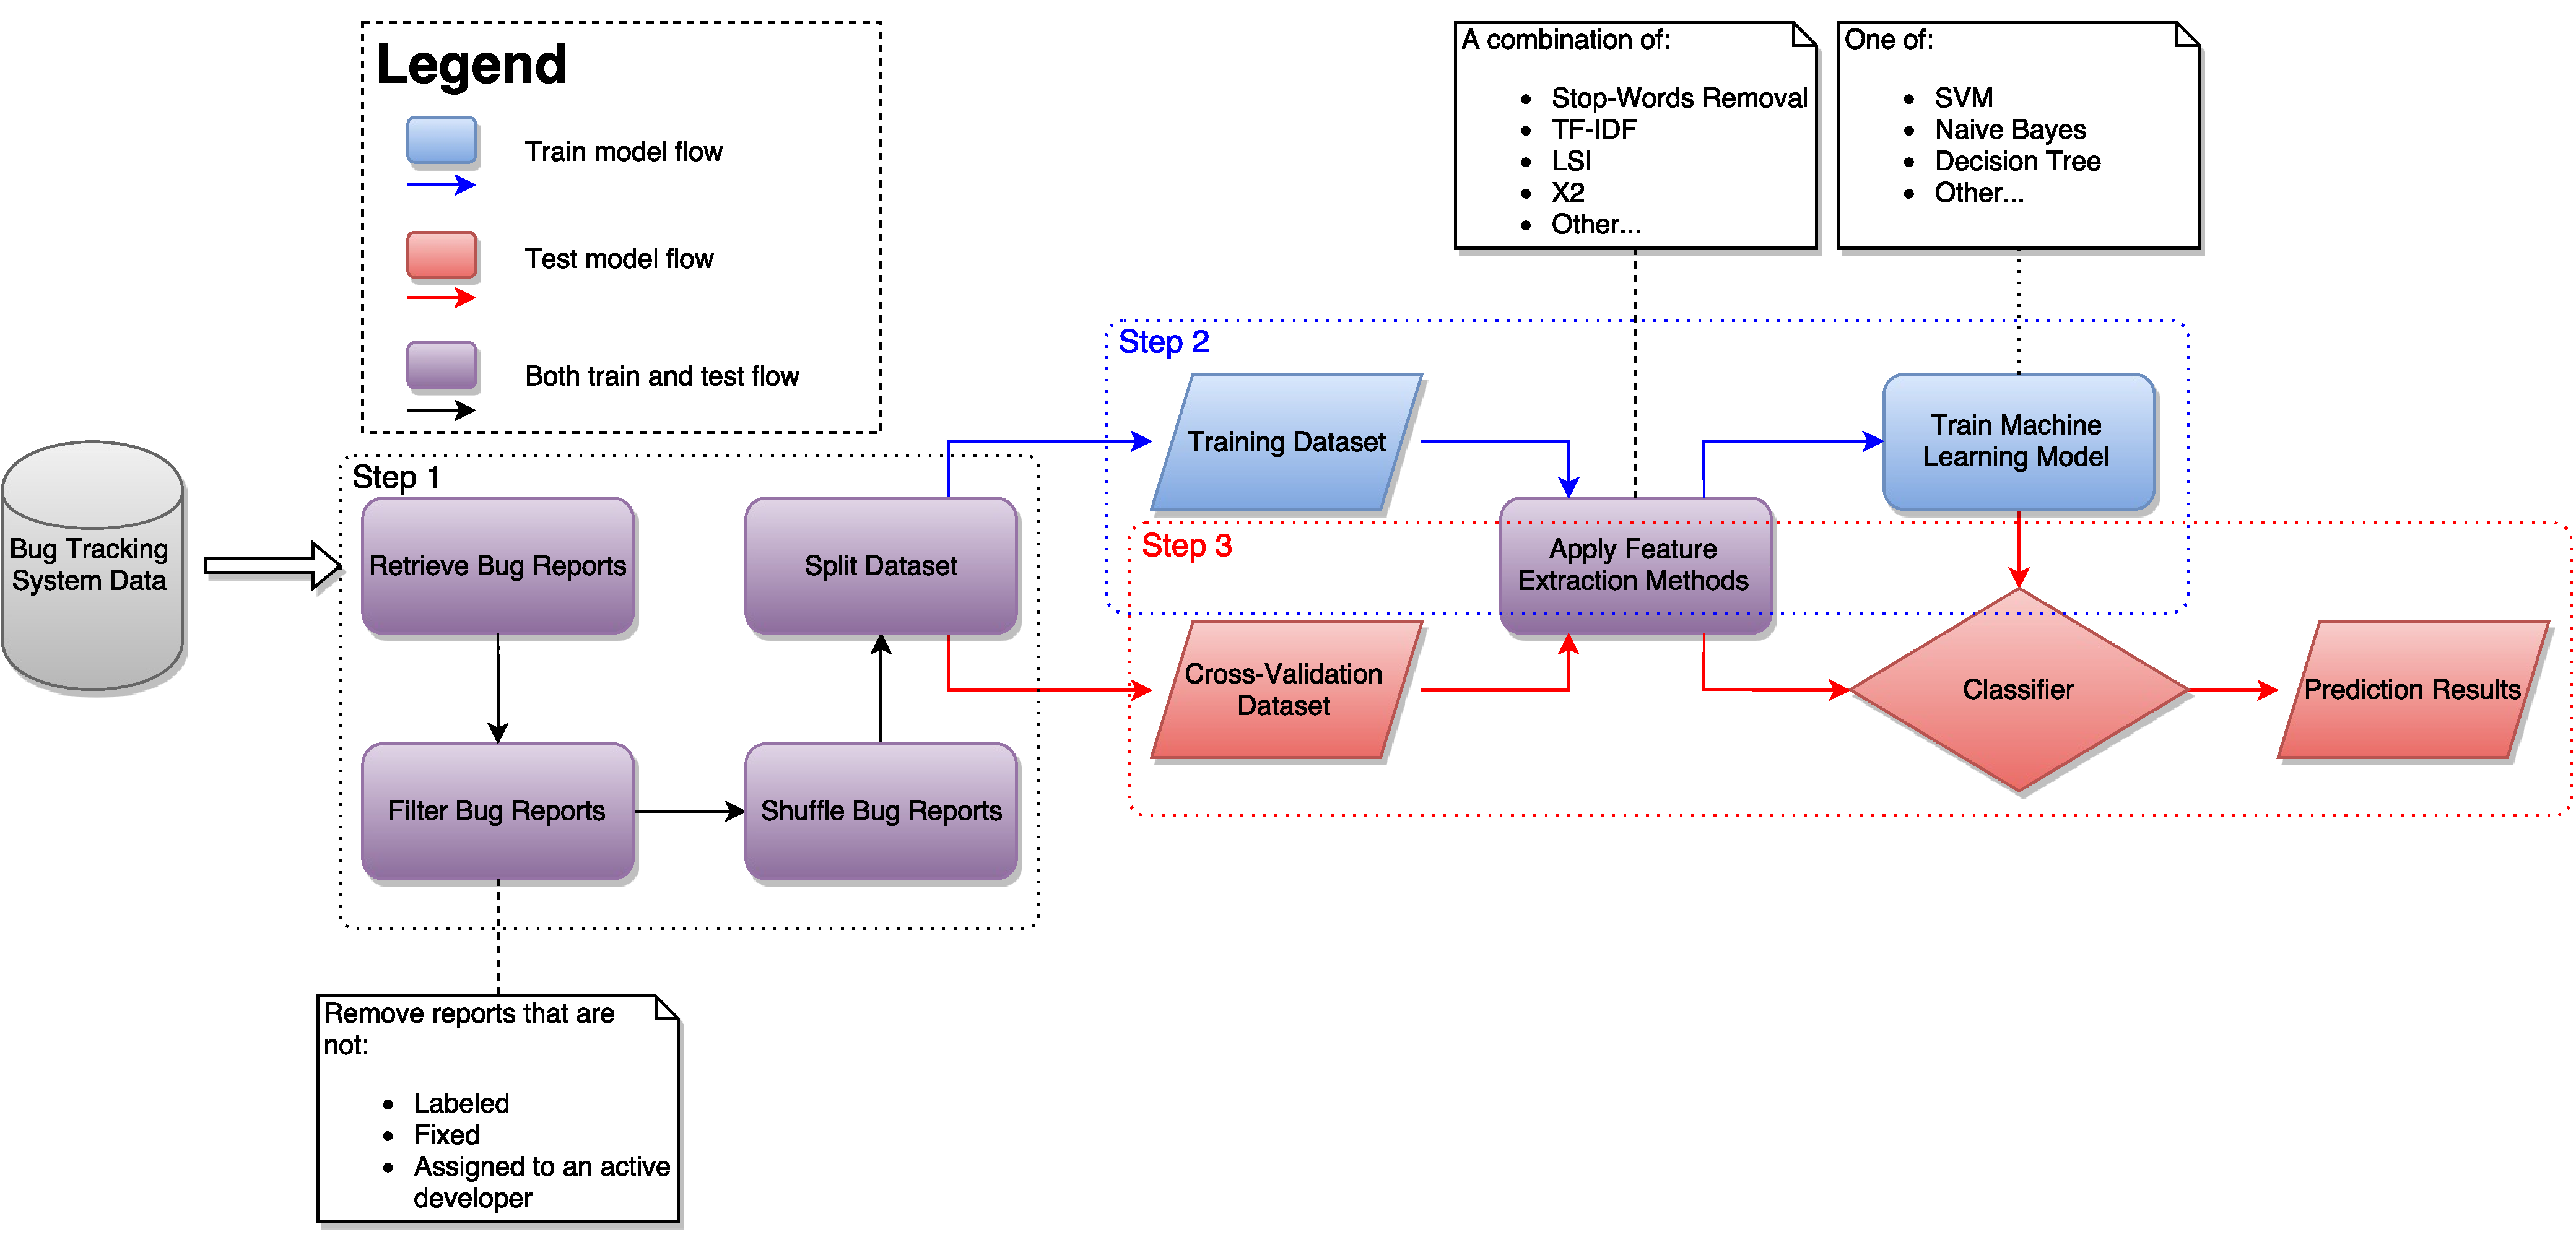
\includegraphics[width=530px, trim=0 5cm 0 0, clip]{./images/flowchart/analysis_flowchart.pdf}
    \caption{Flowchart of the evaluation and analysis process.}
    \label{fig:model.flowchart}
\end{sidewaysfigure}
\clearpage

\section{Datasets}
\label{section:datasets}

To evaluate the performance of a model, we need a set of bug tracking data. One dataset was provided by a private company, but as we eventually want to compare our results with related work, we selected two other open-source projects that are frequently used for training and testing of ML models in related work---Netbeans and Firefox.

In this section, we provide description of these three datasets. We also do a basic analysis of the datasets which will allow us to establish some basic answers to GQM questions \hyperlink{question:4}{4} and \hyperlink{question:5}{5}.

\subsection{Firefox Data}

This dataset is downloaded from Mozilla repository\footnote{https://bugzilla.mozilla.org} from project Firefox. We downloaded all bugs that are in status \texttt{RESOLVED} with resolution \texttt{FIXED} and were created in year 2010 or later. We also removed bugs with field \texttt{assigned\_to} set to \texttt{nobody@mozilla.org} as those tickets were resolved and fixed but not assigned to an actual developer. This yields $9,141$ bugs in total. To get a better comparison with the other datasets, we only use $3,000$ datasets for training and cross-validation that were created between 2010-01-01 and 2012-07-10. This dataset contains $343$ labels (developers). Finally, we remove developers who did not fix at least $30$ bugs, yielding $1,810$ bugs with $20$ developers. The histogram with frequencies of the developers and cumulative distribution is on figure~\ref{fig:datasets.firefox.dist}.

\begin{figure}[htbp]
    \centering
        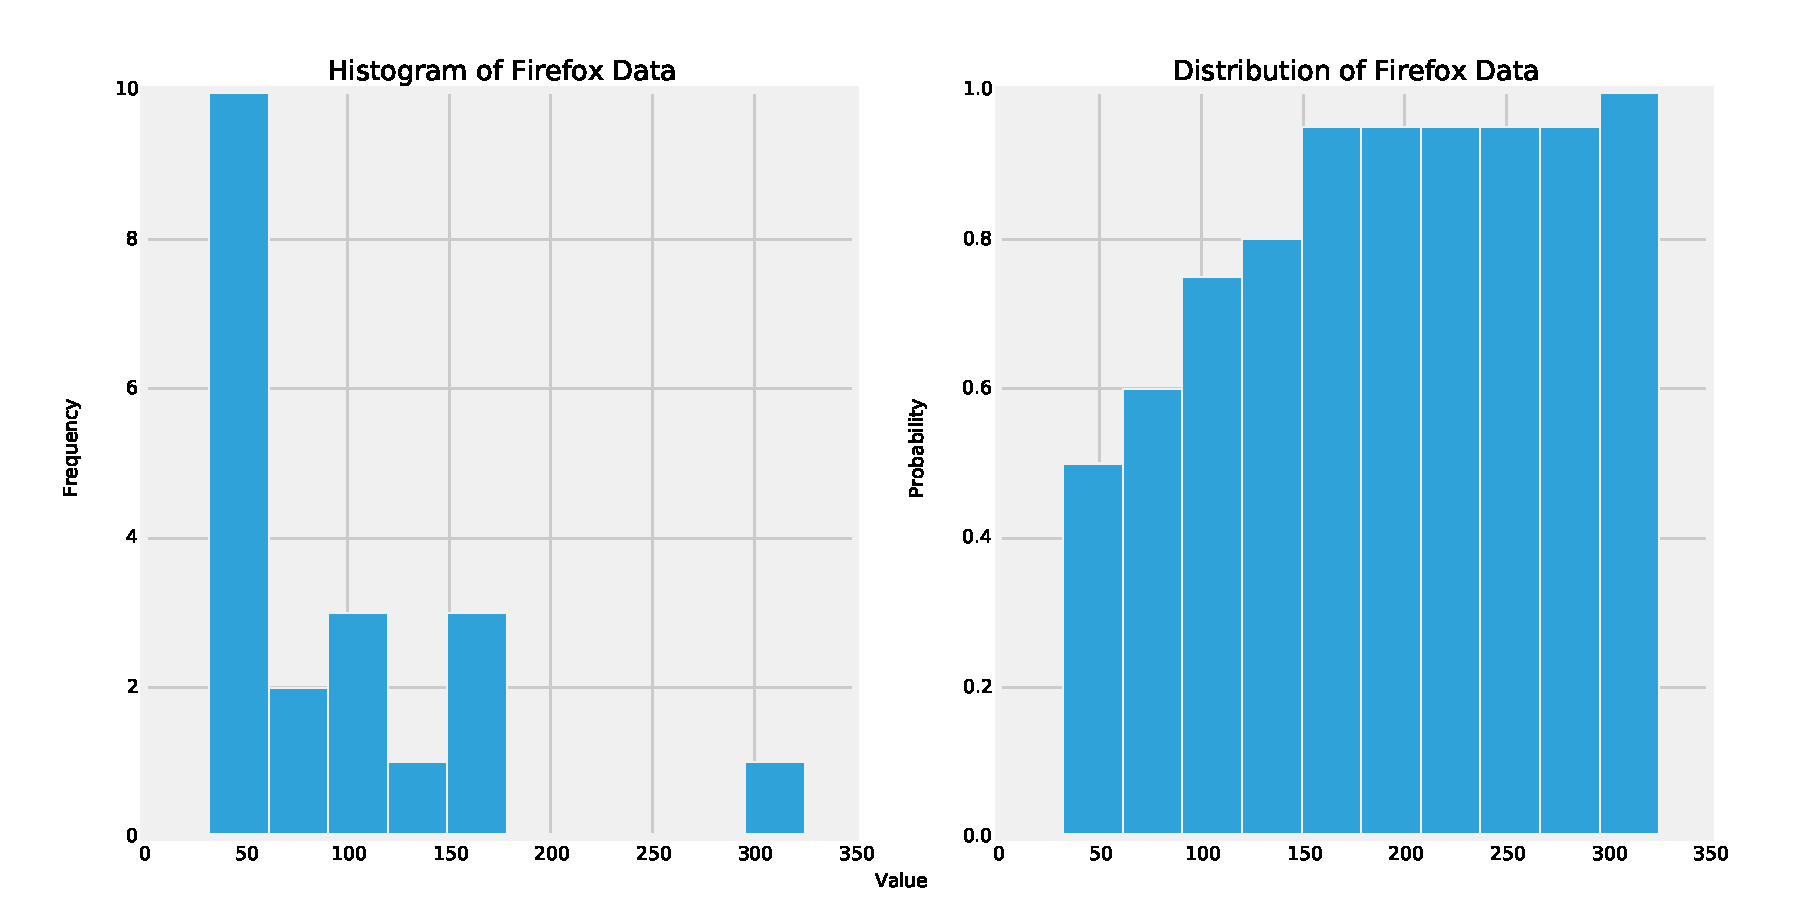
\includegraphics[width=\textwidth]{./images/distribution/firefox.pdf}
    \caption{Histogram and distribution of the Firefox data.}
    \label{fig:datasets.firefox.dist}
\end{figure}

\subsection{Netbeans Data}

Netbeans data were downloaded from Netbeans bug repository\footnote{https://netbeans.org/bugzilla/}. We considered latest $3,000$ bugs that are in status \texttt{RESOLVED} with resolution \texttt{FIXED}. We removed bugs with assignee \texttt{kenai\_tester\_git} (as those were created automatically) resulting in $2,924$ bug reports. These bugs were created between 2014-06-14 and 2015-06-14 and they contain $92$ developers. After removing developers who did not fix at least 30 bugs, the dataset contains $2,528$ reports with $30$ developers. Figure~\ref{fig:datasets.netbeans.dist} is a histogram and distribution of this datasets.

\begin{figure}[htbp]
    \centering
        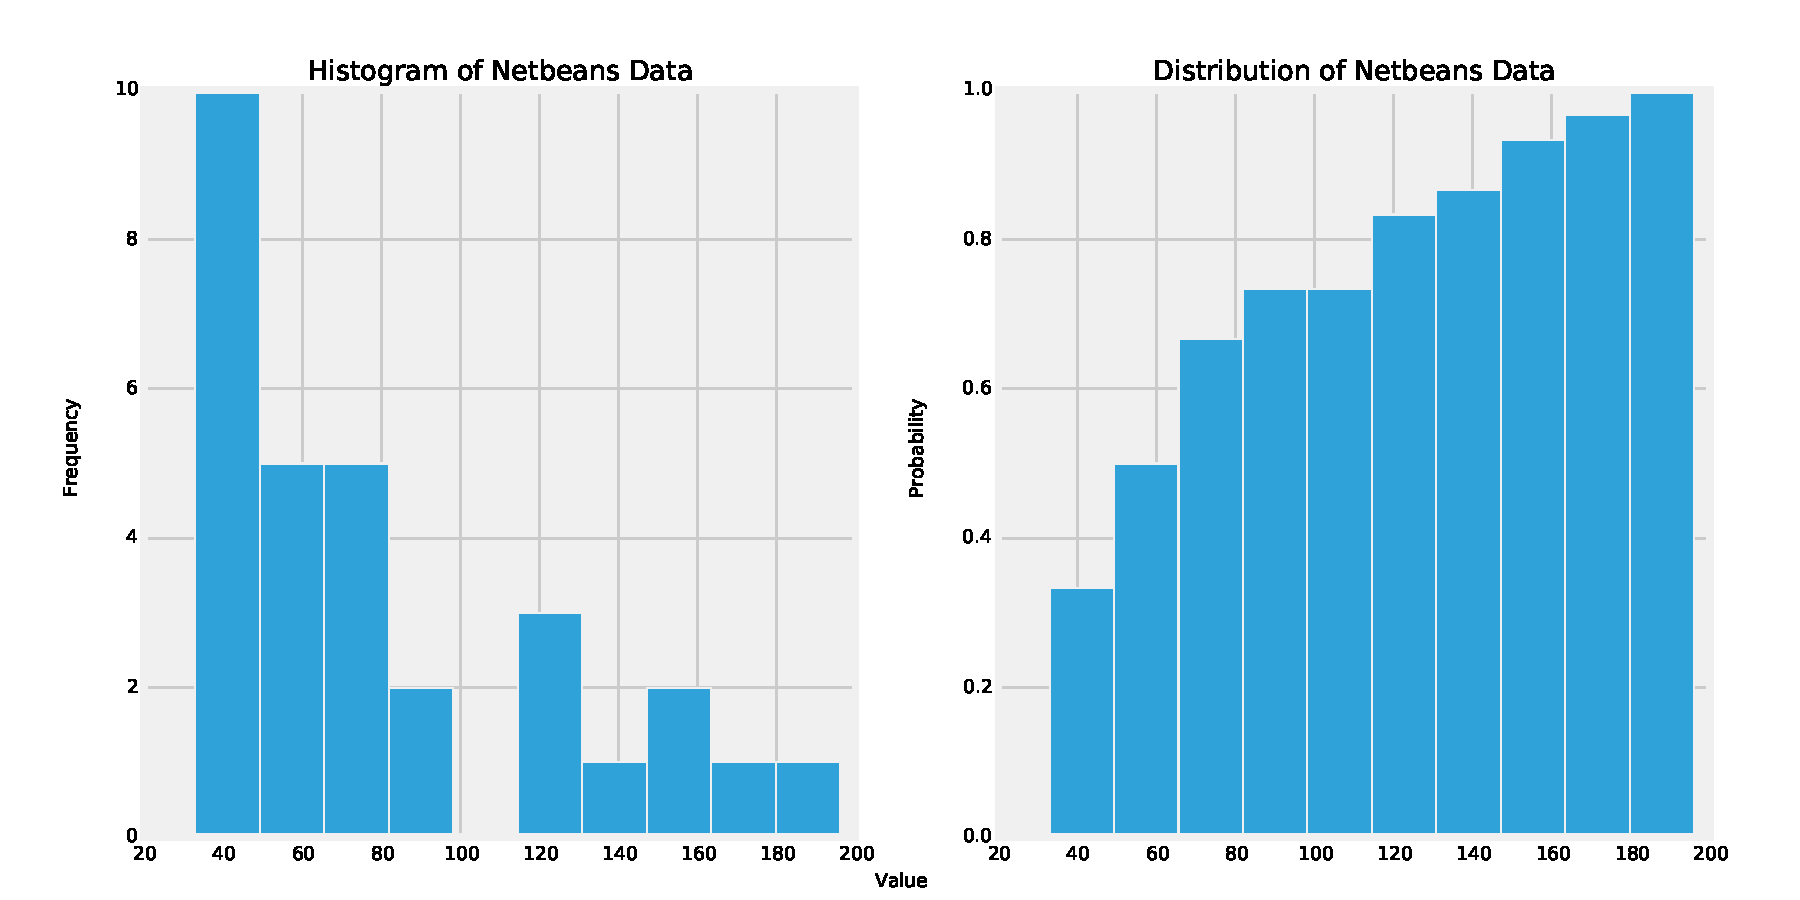
\includegraphics[width=\textwidth]{./images/distribution/netbeans.pdf}
    \caption{Histogram and distribution of the Netbeans data.}
    \label{fig:datasets.netbeans.dist}
\end{figure}

\subsection{Proprietary Data}

The Proprietary dataset was provided by a company that wants to remain anonymous. The provided dataset contains $2,926$ bug reports created between 2012-11-23 and 2015-10-16. Only bug reports that were resolved with assigned developer were considered. There are $110$ developers in this dataset. Only $2,424$ bugs assigned to $35$ developers were retained after removal of developers with less than $30$ fixed bugs. The histogram and probability distribution is pictured on figure~\ref{fig:datasets.proprietary.dist}.

\begin{figure}[htbp]
    \centering
        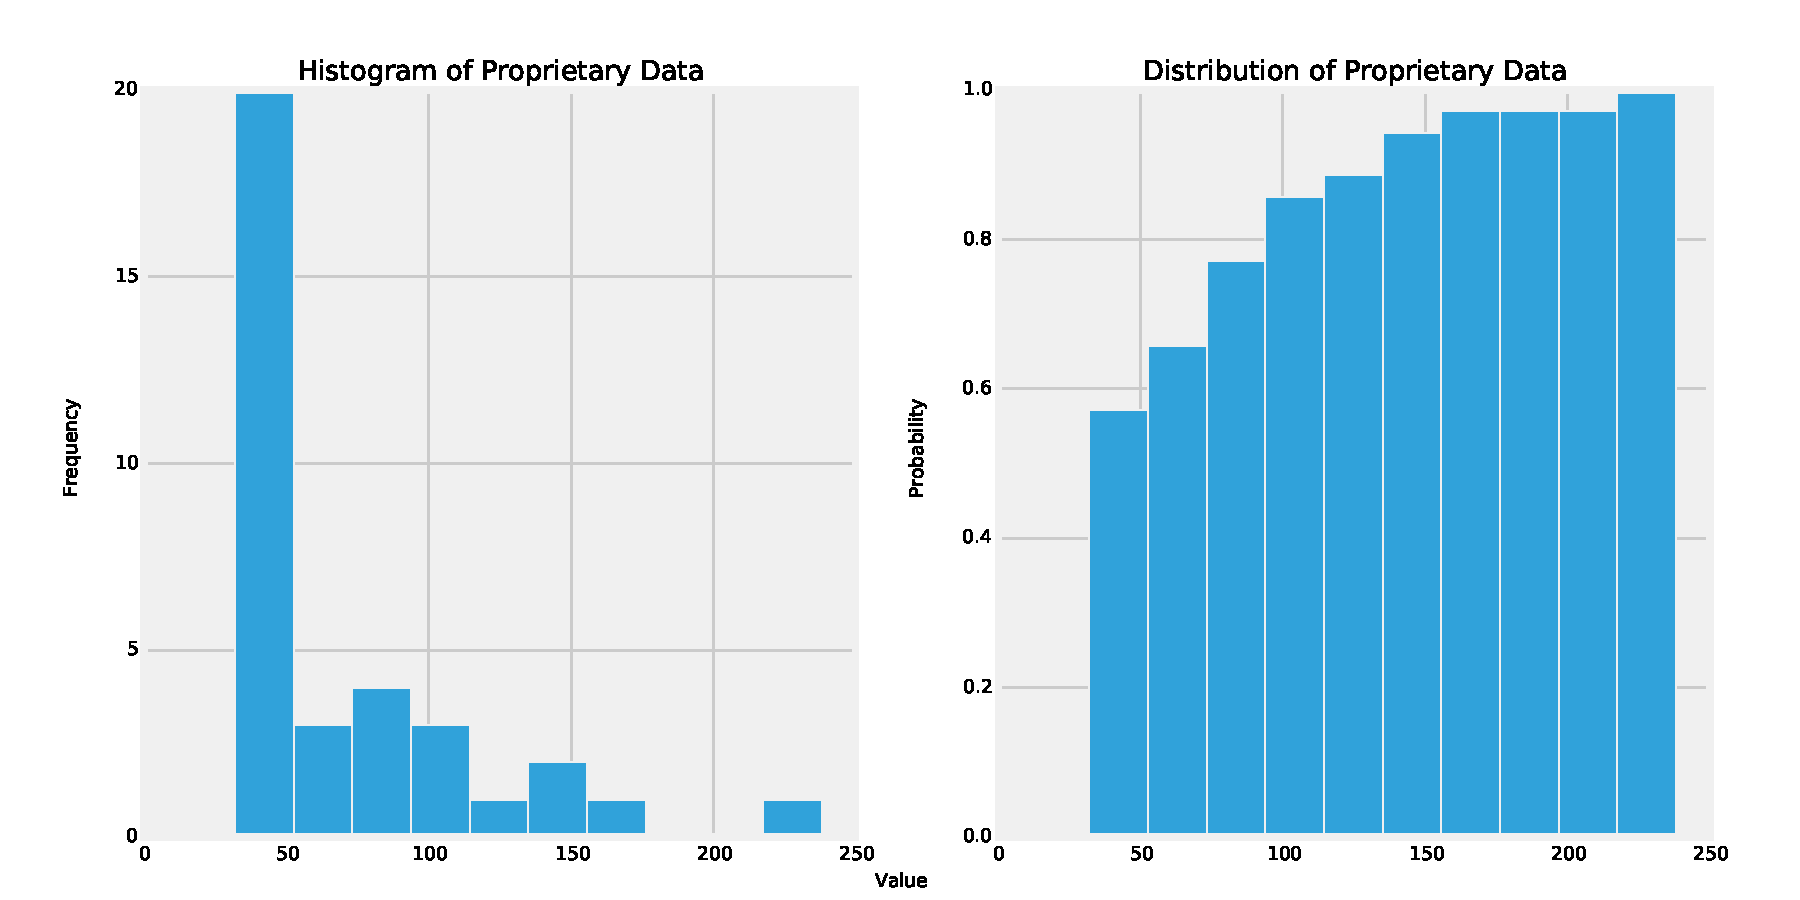
\includegraphics[width=\textwidth]{./images/distribution/proprietary.pdf}
    \caption{Histogram and distribution of the Proprietary data.}
    \label{fig:datasets.proprietary.dist}
\end{figure}

\subsection{Chi-Square Test}

In this section, we test the null hypothesis that two samples are from the same distribution, which will allow us to determine how similar the used datasets are. For this, we use the two-sided alternative of two-sample Chi-Square test. We split the samples from each datasets into five bins and compute the \textit{p-value} for three pairs of samples.

The Chi-Square test with Netbeans and Firefox samples yields p-value of $0.4283$, as p-value~$> 0.05$ we fail to reject the null hypothesis that the two samples are from the same distribution with 5\% level of significance.

The test with Firefox and Proprietary samples returns p-value equal to $0.8648$ so we again fail to reject the null hypothesis. The last test with samples from Proprietary and Netbeans data results in p-value of $0.6182$, which again means the null hypothesis cannot be rejected (with 5\% significance).

\subsection{T-Test}

In the previous section, we tested the hypothesis that the datasets used in this thesis are from the same distribution. We failed to reject the hypothesis with all samples, in this section, we test the null hypothesis that the samples have the same population mean---allowing us to futher learn how statistically similar the datasets are. For that, we have to test the hypothesis that the variances of the samples are the same.

We use the two-sided alternative of the standard independent two-sample t-test to test the null hypothesis that the samples have the same population mean, and the two-sided alternative of the Levene test to test whether the samples have equal population variance. If we reject the null hypothesis of the Levene test, we use the two-sided alternative of the Welch's t-test instead of the standard variant.

First, we test the samples from Firefox and Proprietary datasets. The Levene test yields p-value equal to $0.2730$, as p-value~$> 0.05$, we fail to reject the null hypothesis with 5\% significance level. To test the population mean of the two samples, we therefore have to use the standard independent t-test. The standard independent t-test results in p-value of $0.1954$, which means we fail to reject the null hypothesis of equal population mean of the two samples with 5\% significance.

Second, we test the samples from Firefox and Netbeans repositories. As the Levene test returns p-value equal to $0.4397 > 0.05$, we fail to reject the null hypothesis of equal population variances (5\% significance). The p-value of the standard independent t-test on these two samples is equal to $0.5924$, which means we fail to reject the null hypothesis of equal population means with 5\% significance.

Last samples we test are from Netbeans and Proprietary datasets. The p-value of the Levene test for these two samples is $0.6007$ thus we fail to reject the null hypothesis of equal variances. The p-value of the standard independent t-test is equal to $0.3061$, which again means we have to reject the null hypothesis that the two samples have the same population mean (5\% significance).

\subsection{Conclusion}

Our basic analysis of the datasets allows us to partially answer two questions established in chapter~\ref{chapter:methodology}. The similarity in the distributions and means of the datasets suggests that our models will work on all datasets regardless of parameter values (\hyperlink{question:4}{Q4}). The results of our chi-square test and t-test imply there is little difference between proprietary and open-source data, partially answering~\hyperlink{question:5}{Q5}. Our confidence in these answers will be further refined when we evaluate our models and datasets.

\section{Window Size}
\label{section:window-size}

The size of the time window is an important question that needs to be addressed when dealing with machine learning. A naive approach uses all samples from a dataset to train the classifier, but a more advanced approach considers what effect does the size of the window have on the data and how it can improve the performance. In this section, we try to address this concern by evaluating the performance of the classifier for different sizes of the window (addressing~\hyperlink{question:6}{Q6}).

To determine weather a different size of the window helps the performance is a difficult endeavour, we attempt it by employing three different approaches, each approach can be described by two properties:

\begin{enumerate}
 \item Fixed number of bugs per period, variable size of the train set
 \item Variable number of bugs per period, fixed size of the train set
 \item Variable number of bugs per period, variable size of the train set
\end{enumerate}

The Firefox dataset is used for testing of all approaches. The model that is applied is Support Vector Machine with TF--IDF weighing---the reason for this choice will be clear in the evaluation part of this chapter, the choice is not really important for the analysis.

\subsection{First Approach}

In the first approach, we first remove all bugs from the whole dataset that were fixed by developers with less than 20 fixed bugs. Then we split the remaining dataset into 8 bins. First bin contains 1000 randomly selected bug reports from period 1. All subsequent bins (2-8) contain 500 randomly selected reports from periods 2-8. There are 8 periods, first period is about one year long, all the other periods are about half a year long each. All periods combined add up to the time span of the whole dataset and each $n+1$ period contains bugs older than $n$ period. We train the classifier on period 1, then 1-2, 1-3, 1-4, 1-5, 1-6, 1-7 and 1-8. We test each trained classifier on the same cross-validation set of 300 bug reports that are newer than bugs in period 1.

The disadvantage of this approach is that you select fixed number of bugs from each period. In real world, each period can contain different number of bug reports based e.g. on season. Another disadvantage is that you remove developers that do not meet the criteria of 20 bugs fixed based on the whole dataset. If some developers were very active in the past but are no longer very relevant, they will not be removed from a dataset that is constructed from periods in which the developer no longer fulfills the criteria.

The result is visualized on figure~\ref{fig:window.firefox.1a}. You can see that about the best result is achieved with the size of the window equal to 30 months. Unfortunately, the performance of the classifier for other sizes is very similar and the results are therefore inconclusive.

\begin{figure}[htbp]
    \centering
        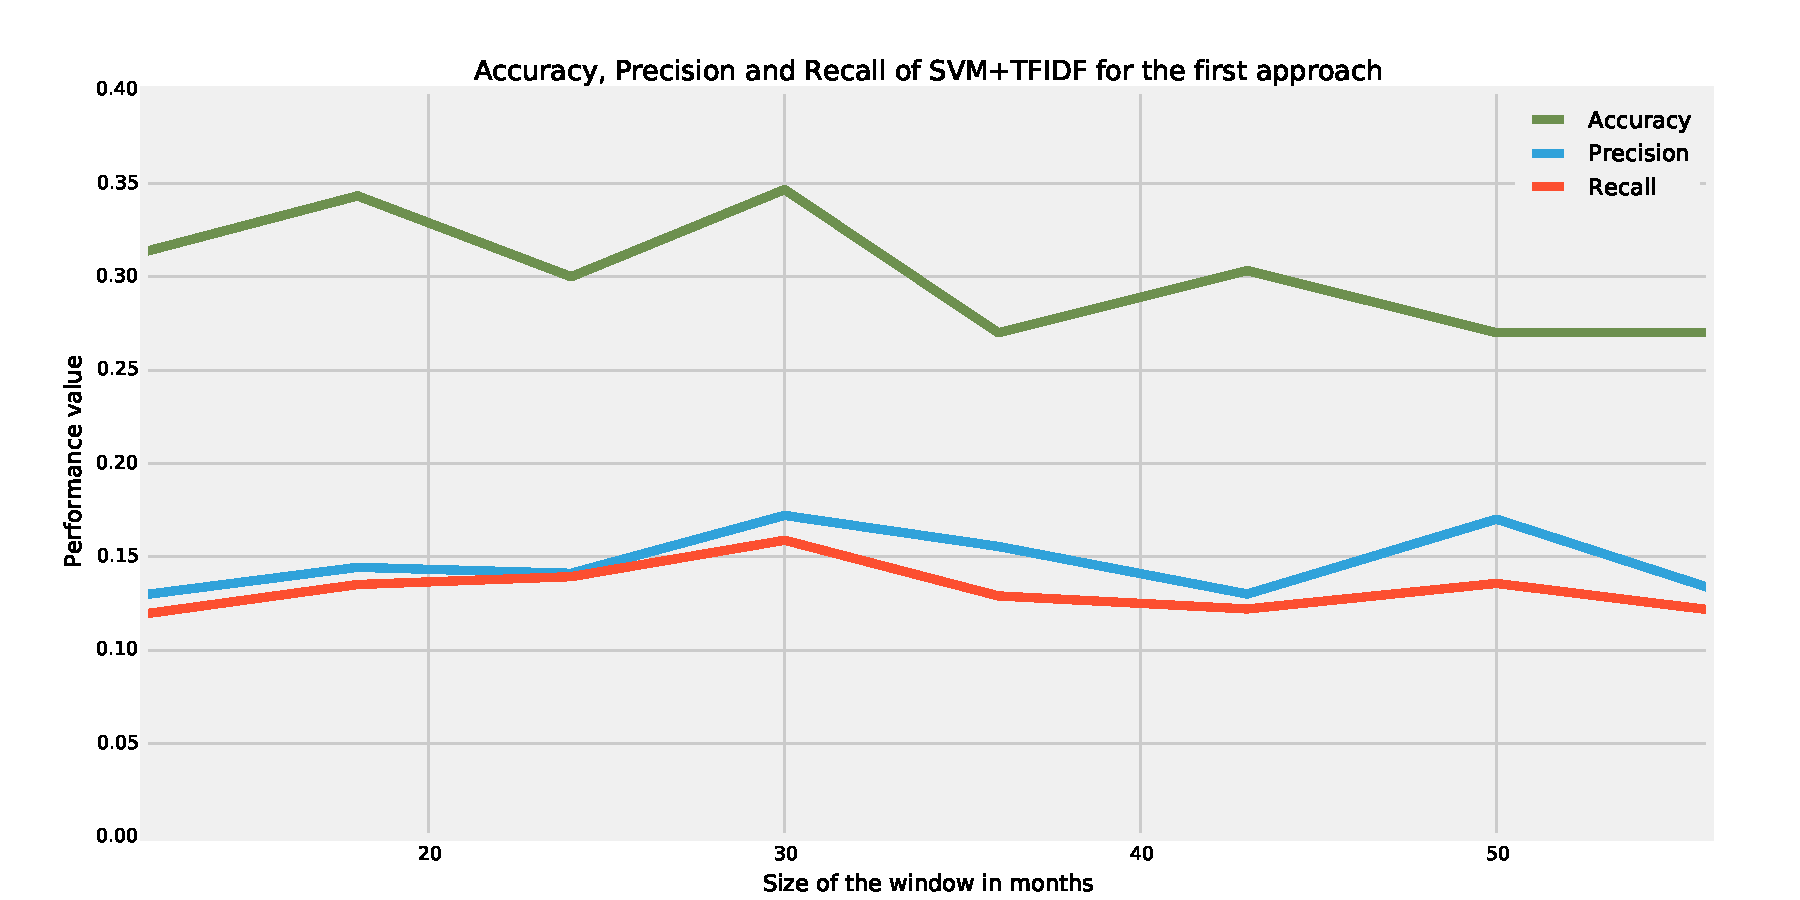
\includegraphics[width=\textwidth]{./images/window_size/firefox_1a.pdf}
    \caption{Performance of the classifier for different sizes of the window, 1st approach.}
    \label{fig:window.firefox.1a}
\end{figure}

\subsection{Second Approach}

In the second approach, we employ the same periods, except period 1 that is about 15 months long. Another difference is that each train set contains 3000 randomly selected bug reports from period 1, 1-2, 1-3 etc. and the size of the sample is in this case therefore fixed, what is different is the period from which they were selected. From each bin, all bug reports that were fixed by a developer with less than 30 fixed bugs within the same train set are removed. We also remove all bug reports from cross-validation set that are not in the train set. We do this to get more relevant results from macro-averaged metrics, because otherwise the result of such metrics would be very close to zero.

The disadvantage of the second approach is that it does not really tell us what size of the window can be used to get the best performance. What it shows is whether the size of the window from which an equal size of sample is selected matters.

Figure~\ref{fig:window.firefox.2a} shows the plot of this approach. The performance decreases as the size of the window increases, which is expected. Precision and recall however increases when the size of the window is around 45 months.

\begin{figure}[htbp]
    \centering
        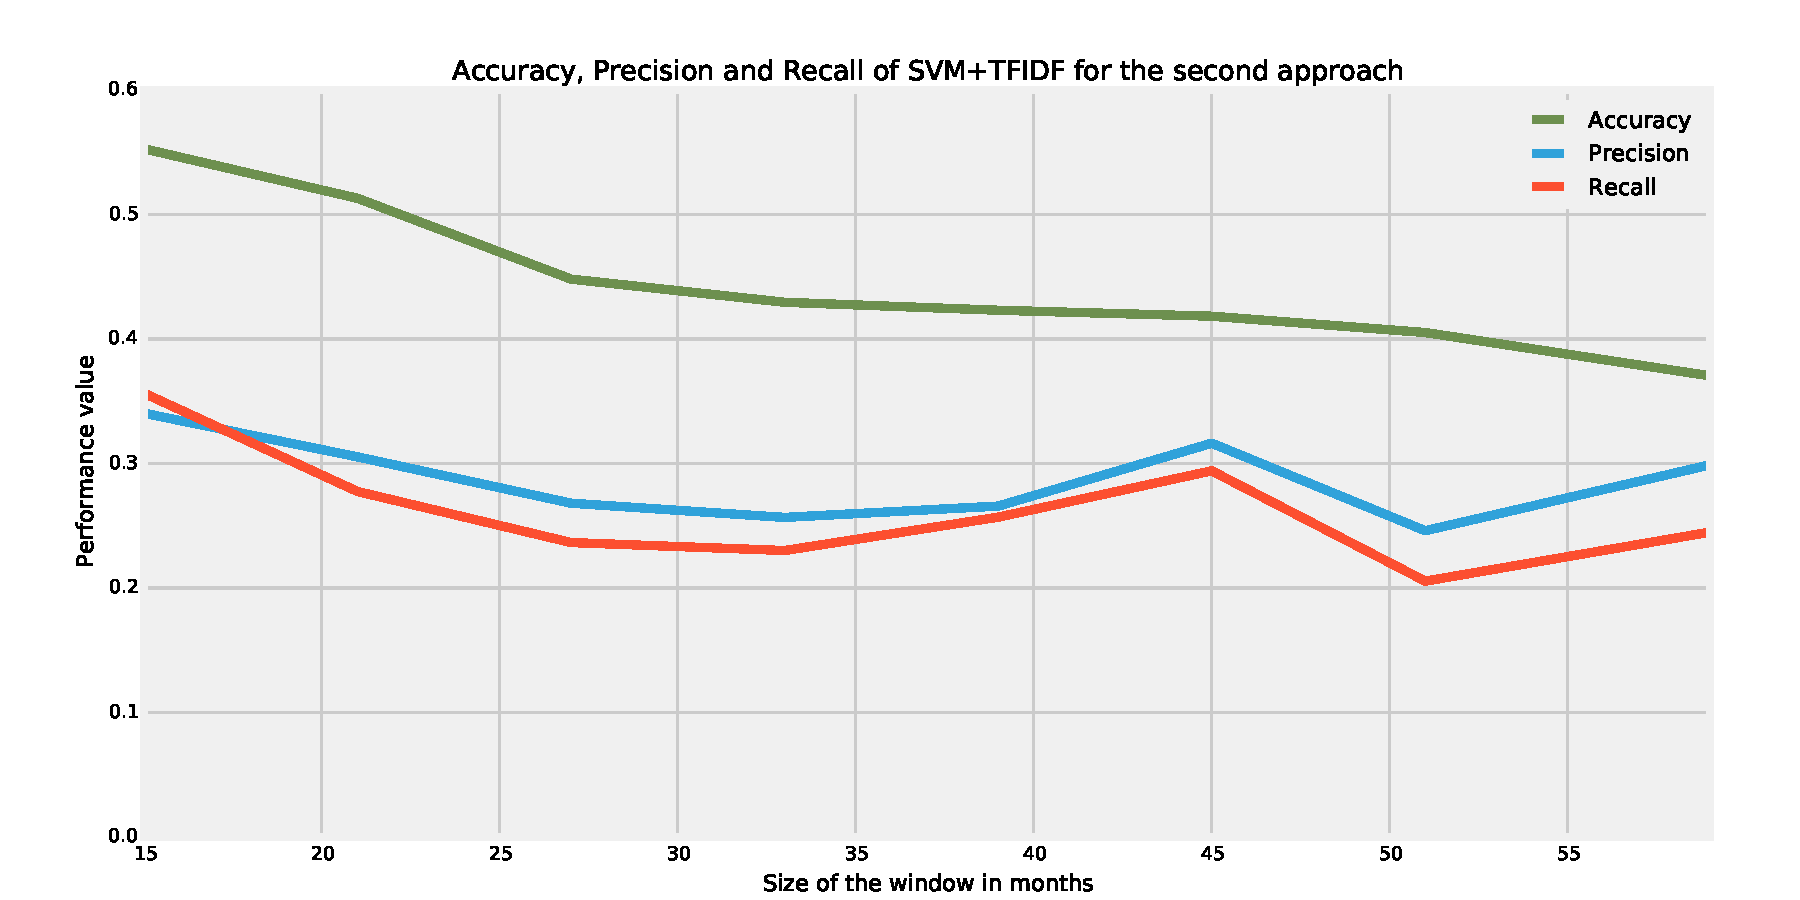
\includegraphics[width=\textwidth]{./images/window_size/firefox_2a.pdf}
    \caption{Performance of the classifier for different sizes of the window, 2nd approach.}
    \label{fig:window.firefox.2a}
\end{figure}

\subsection{Third Approach}

Finally, in the third approach, we again use the same periods as in the second approach. The difference is that we select all bug reports as train set.

The advantage is that this approach is closest to reality (no random selection). The disadvantage is, however, that the results are skewed by a variable number of samples in each period. The last major disadvantage is that the number of classes (developers) increases significantly each time samples from the next period are added. Figure~\ref{fig:window.firefox.3a} shows the plot of this approach.

\begin{figure}[htbp]
    \centering
        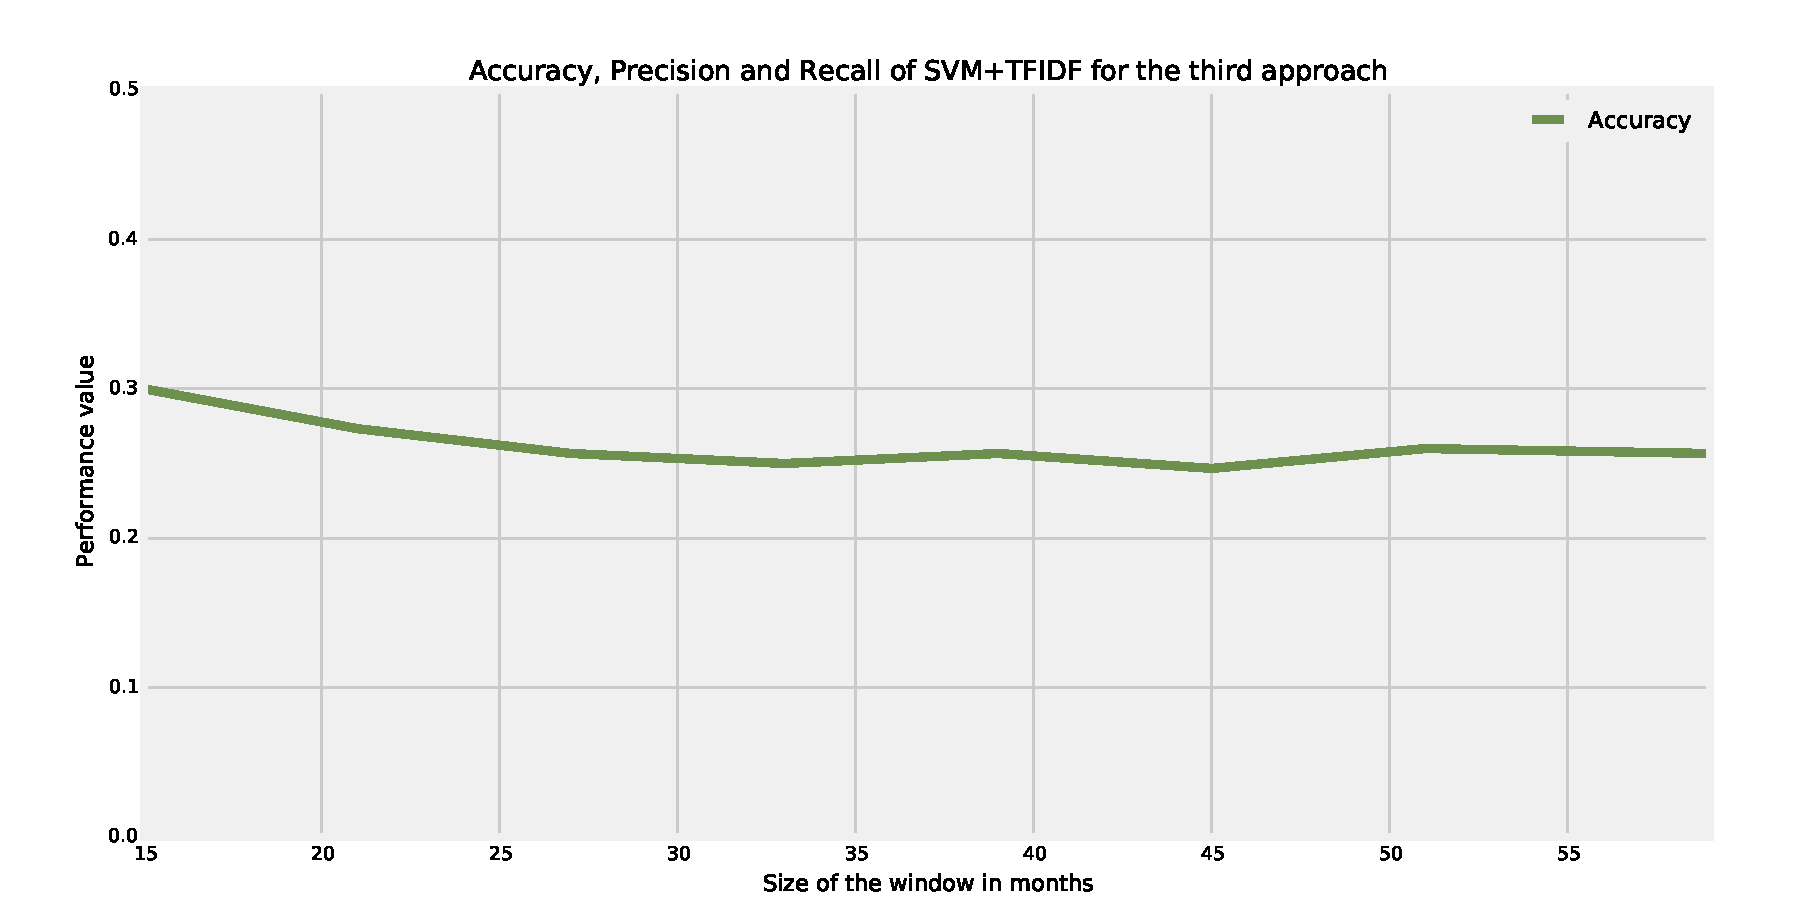
\includegraphics[width=\textwidth]{./images/window_size/firefox_3a.pdf}
    \caption{Performance of the classifier for different sizes of the window, 3rd approach.}
    \label{fig:window.firefox.3a}
\end{figure}

\subsection{Conclusion}

Even after the application of all three approaches, it is hard to draw a concrete conclusion about the window size effect on the performance. The results do seem to imply that there are no significant differences in terms of performance between different time-windowing strategies (\hyperlink{question:6}{Q6}), but to increase the confidence of these results, it would be necessary to do a more thorough analysis with possibly more approaches or different processing strategy.

\section{Topic Analysis}

In this section, we analyze the distribution of topics with respect to time for proprietary and Firefox datasets in order to further determine the differences or similarities of open-source and proprietary datasets. We model 10 topics using Latent Dirichlet Allocation (LDA) in our approach.

The plots show the prevalence of topics each month where a different shade of gray represents a different topic. In terms of our GQM methodology, this section contributes to the answer of questions~\hyperlink{question:4}{4} and~\hyperlink{question:5}{5} (described in chapter~\ref{chapter:methodology}).

\subsection{Firefox Data}

All our Firefox bug reports were created within 62 months. You can see the distribution on figure~\ref{fig:distribution.firefox.topic}. The plot shows that the distribution of topics is quite significantly different each month with two dominant topics. The distribution of the topics seems to oscillate periodically which could be an indication of a release cycle of major Firefox versions, which would not be surprising as many projects have a predetermined periodic release cycle.

\begin{figure}[htbp]
    \centering
        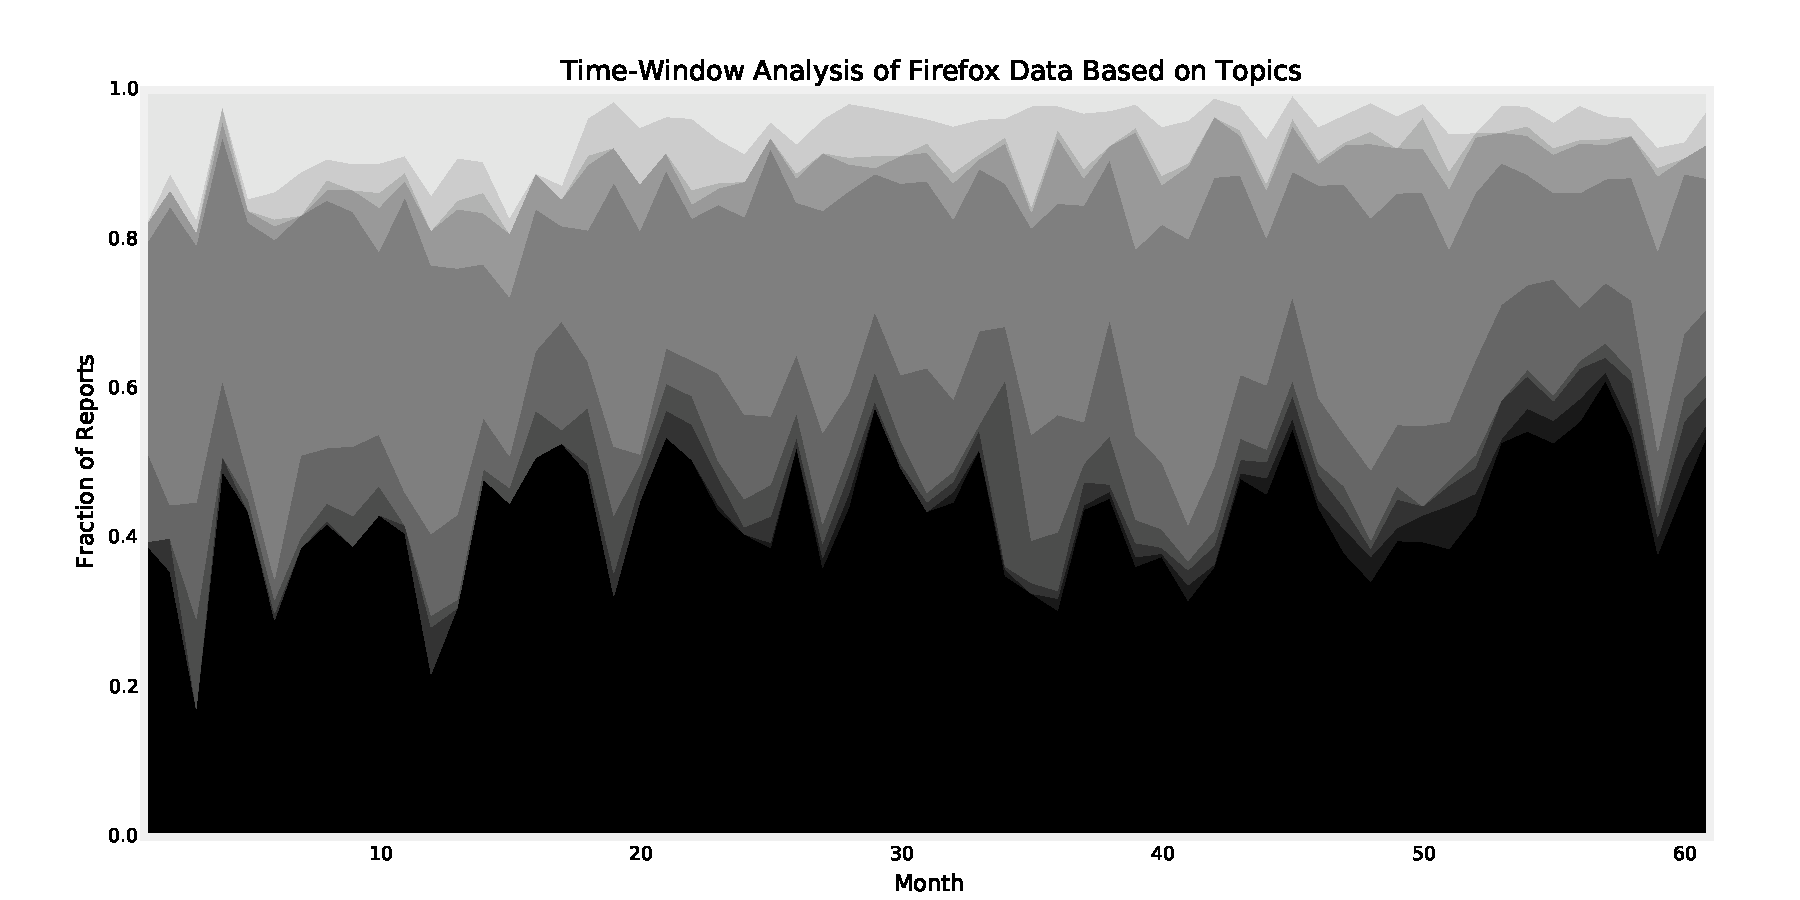
\includegraphics[width=\textwidth]{./images/topic_component_distribution/firefox_topic_10.pdf}
    \caption{Topic analysis of Firefox data.}
    \label{fig:distribution.firefox.topic}
\end{figure}

\subsection{Proprietary Data}

The proprietary bug reports were created within 36 months. You can see the distribution on figure~\ref{fig:distribution.prop.topic}. The plot again shows that the distribution of topics in the proprietary datasets is quite different each month, although their dominance changes quite a lot as well. The first few months are dominated by a single topic, but its significance later drops as other topics take over. Contrary to the Firefox distribution, there does not seem to be an indication of a release cycle, instead, each topic seems to be important only for a limited period of time.

\begin{figure}[htbp]
    \centering
        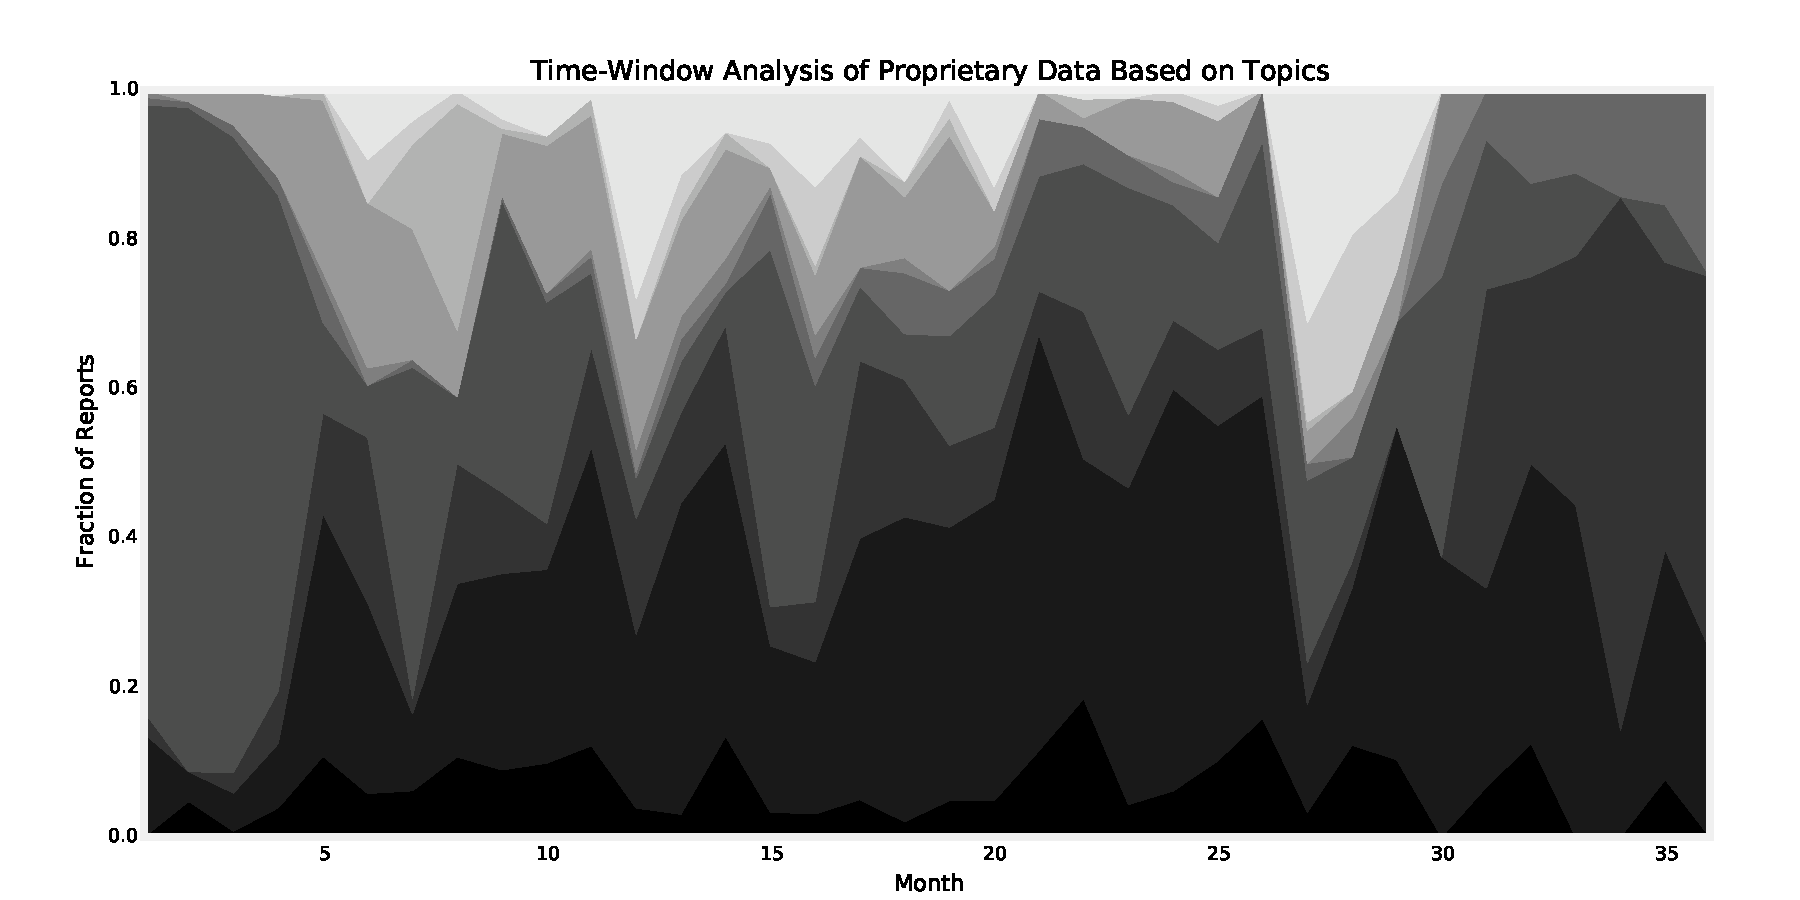
\includegraphics[width=\textwidth]{./images/topic_component_distribution/proprietary_topic_10.pdf}
    \caption{Topic analysis of the proprietary data.}
    \label{fig:distribution.prop.topic}
\end{figure}

\subsection{Conclusion}

The topic analysis presented in this section does suggest some difference in topic distribution (with respect to time). It is not surprising as different projects are developed different ways, the application of different software development methodologies (scrum, waterfall, TDD etc) is one of the factors that are likely to affect the results. In terms of~\hyperlink{question:4}{Q4}, these results decrease our confidence that our models work for all datasets equally without the need to tune their parameters. As far as~\hyperlink{question:5}{Q5} is concerned, the difference between the Firefox and proprietary datasets can be explained by different development processes.

\section{Baseline}
\label{section:baseline}

In this section, we establish a baseline for our models (addressing~\hyperlink{question:1}{Q1}). Our baseline is very simple, the number of bug report that is assigned to each developer is counted and the developer with the highest number of assigned bugs is selected as a prediction for each subsequent call of the \texttt{predict} function.

Figure~\ref{fig:models.firefox.stopwords} shows the performance of the baseline model on Firefox data. While the accuracy of this model is relatively high (18\%), the precision and recall values are much lower (1\% and 5\%), which can be explained by the way macro-averaged metrics work, see metrics in chapter~\ref{chapter:methodology}.

\section{Stop-Words Removal}

Stop-words removal is a technique that can increases performance of the model. In this section, we determine whether the increase is significant enough to use it for subsequent comparisons of models.

\begin{figure}[htbp]
    \centering
        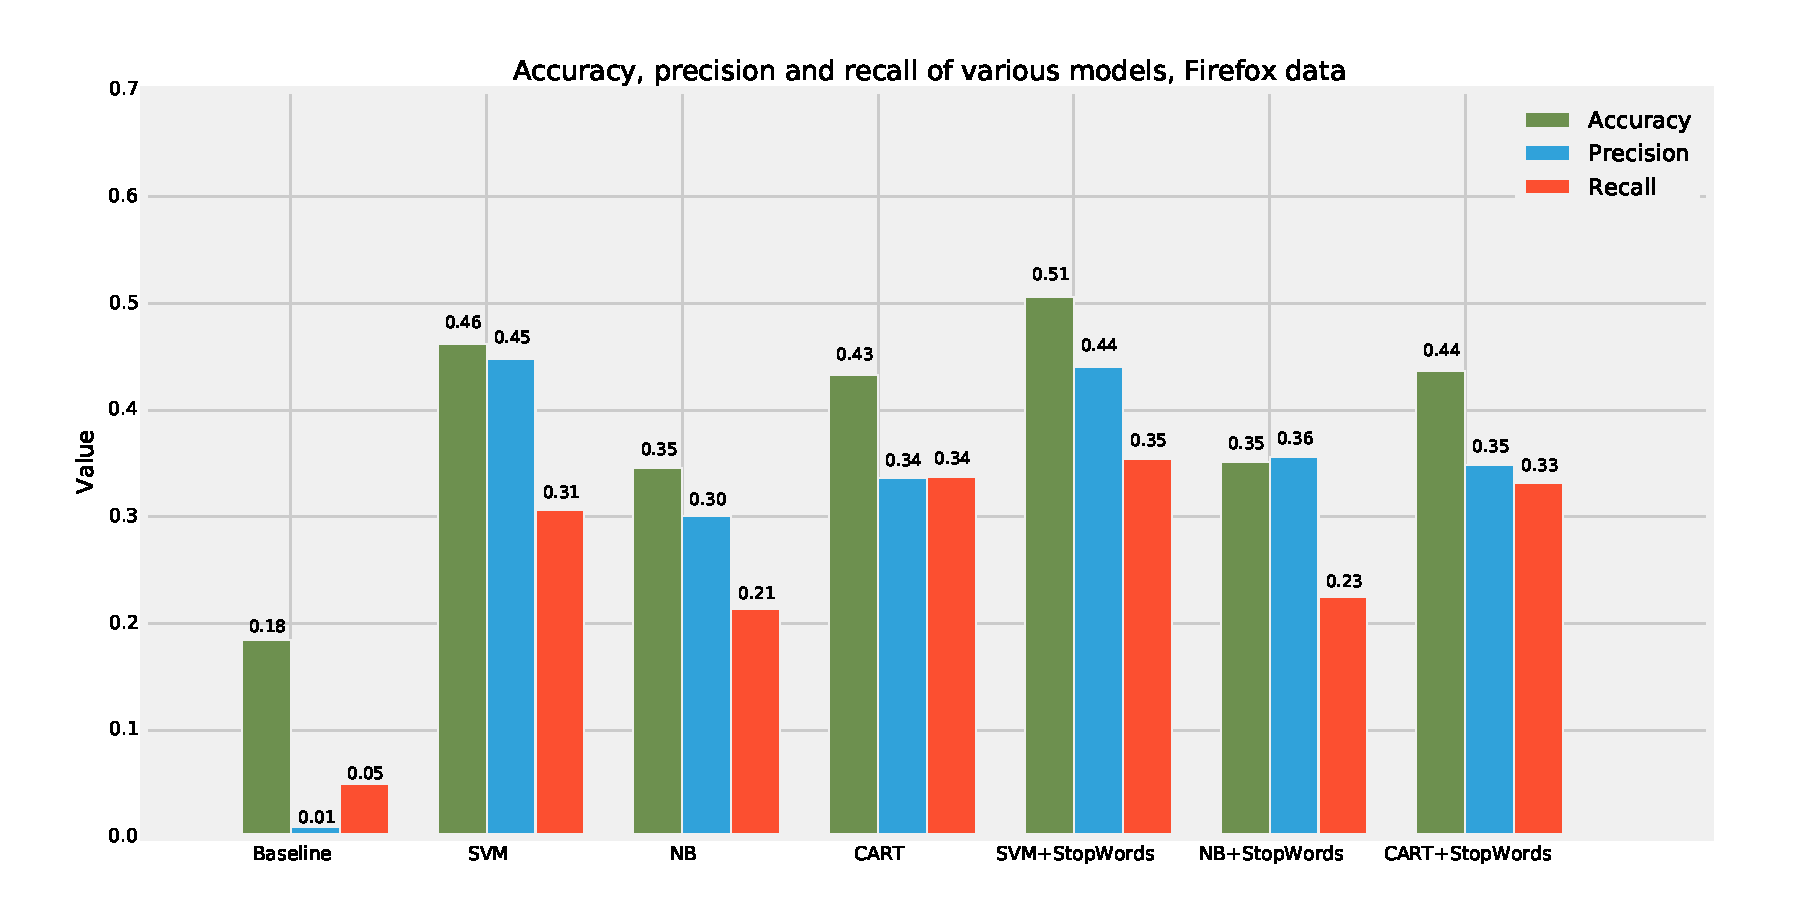
\includegraphics[width=\textwidth]{./images/comparison_of_models/firefox_0.pdf}
    \caption{Stop-words removal on Firefox data.}
    \label{fig:models.firefox.stopwords}
\end{figure}

Figure~\ref{fig:models.firefox.stopwords} shows the increase in performance after all stop-words were removed from the feature vector of the Firefox data. You can see that the performance of the classifier slightly increased on all models. Accuracy increased by 3\%, 0\% and 1\% on SVM, Naive Bayes and CART model respectively. Precision value of the SVM model decreased by 1\% but increased by 6\% with Naive Bayes model and by 1\% with CART. Finally, Recall values of SVM and Naive Bayes increased by 4\% and 2\% respectively while it slightly decreased with the CART model by about 1\%.

The results of the other datasets were similar in nature. We therefore conclude that the performance boost of stop-words removal is significant enough to warrant better results, which matches the conclusion of Čubranić and Murphy~\cite{Murphy} (see chapter~\ref{chapter:related-work}). Thus, in our evaluation, we always use stop-words removal in combination with other feature extraction methods.

\section{Comparison of Models}

In the following text, comparison of the models is presented. We show the \hyperlink{metric:a}{accuracy}, \hyperlink{metric:p}{precision} and \hyperlink{metric:r}{recall} of these models on three datasets. Based on related work (chapter~\ref{chapter:related-work}), we decided to compare three models---Naive Bayes, CART and Support Vector Machine. The theoretical background of these models is covered in chapter~\ref{chapter:background}. The metrics we use are explained in chapter~\ref{chapter:methodology}.

In terms of GQM, this section attempts to answer question~\hyperlink{question:2}{2} (how many times the model predicts the correct assignee), question~\hyperlink{question:3}{3} (how many times the model predicts the correct assignee if the distribution of bug reports is unbalanced) and question~\hyperlink{question:4}{4} (if the model with the same parameters works with all projects). The answers are addressed in the conclusion of this section.

\subsection{Firefox Data}

On Figure~\ref{fig:results.models.firefox}, you can see the performance of the chosen models on Firefox data. The SVM model with TF-IDF weighing achieves the best performance with accuracy of 57\%. Its precision and recall also outperforms all the other approaches with values of 51\% and 45\%. The same model with LSI takes second place. The only model other than SVM that approaches SVM with it's performance is CART, especially with TF-IDF weighing.

\begin{figure}[htbp]
    \centering
        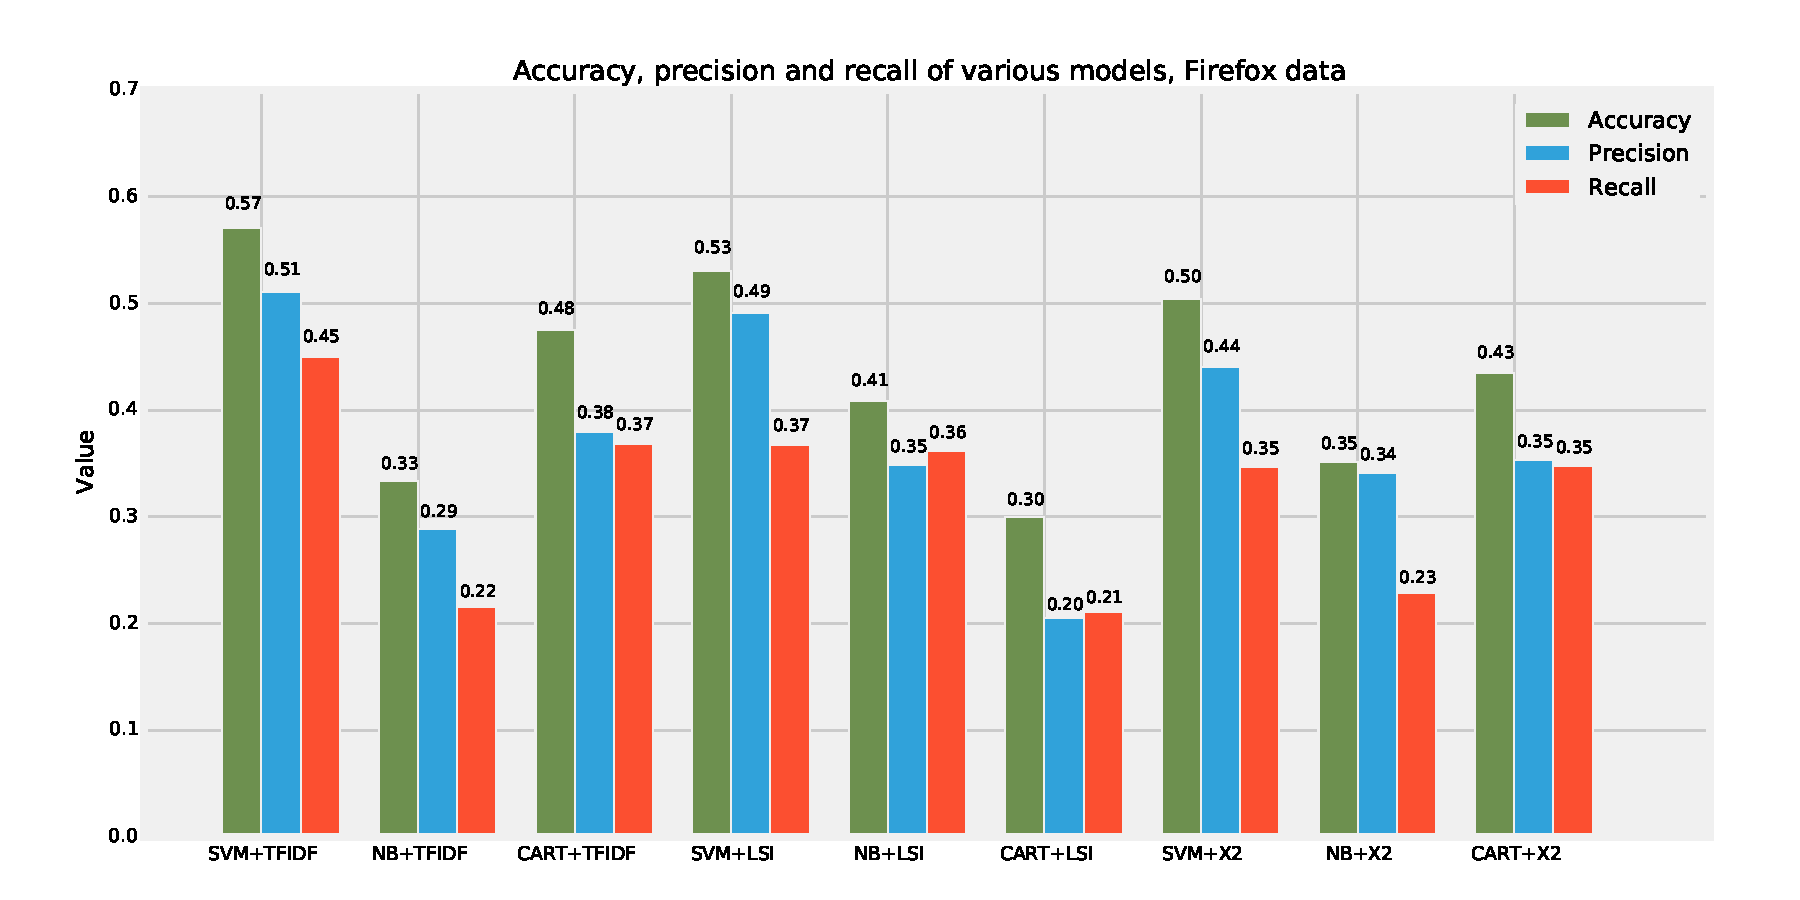
\includegraphics[width=\textwidth]{./images/comparison_of_models/firefox.pdf}
    \caption{Comparison of models on Firefox data.}
    \label{fig:results.models.firefox}
\end{figure}

\subsection{Netbeans Data}

The performance of the models on Netbeans data is shown on Figure~\ref{fig:results.models.netbeans}. It is clear that the SVM model with TF-IDF weighing performs best even on the Netbeans data, although in this case the LSI feature extraction technique does not seem to perform as well as in the previous case. The accuracy, precision and recall of the approach are 53\%, 53\% and 49\% respectively. Sole SVM model and SVM+$\chi^2$ model perform similarly as far as precision is concerned, while the accuracy and recall values are lagging behind by a considerable margin. None of the other models offer better performance than even sole SVM model on this data, which suggests that SVM is a very good choice for automatic bug assignment.

\begin{figure}[htbp]
    \centering
        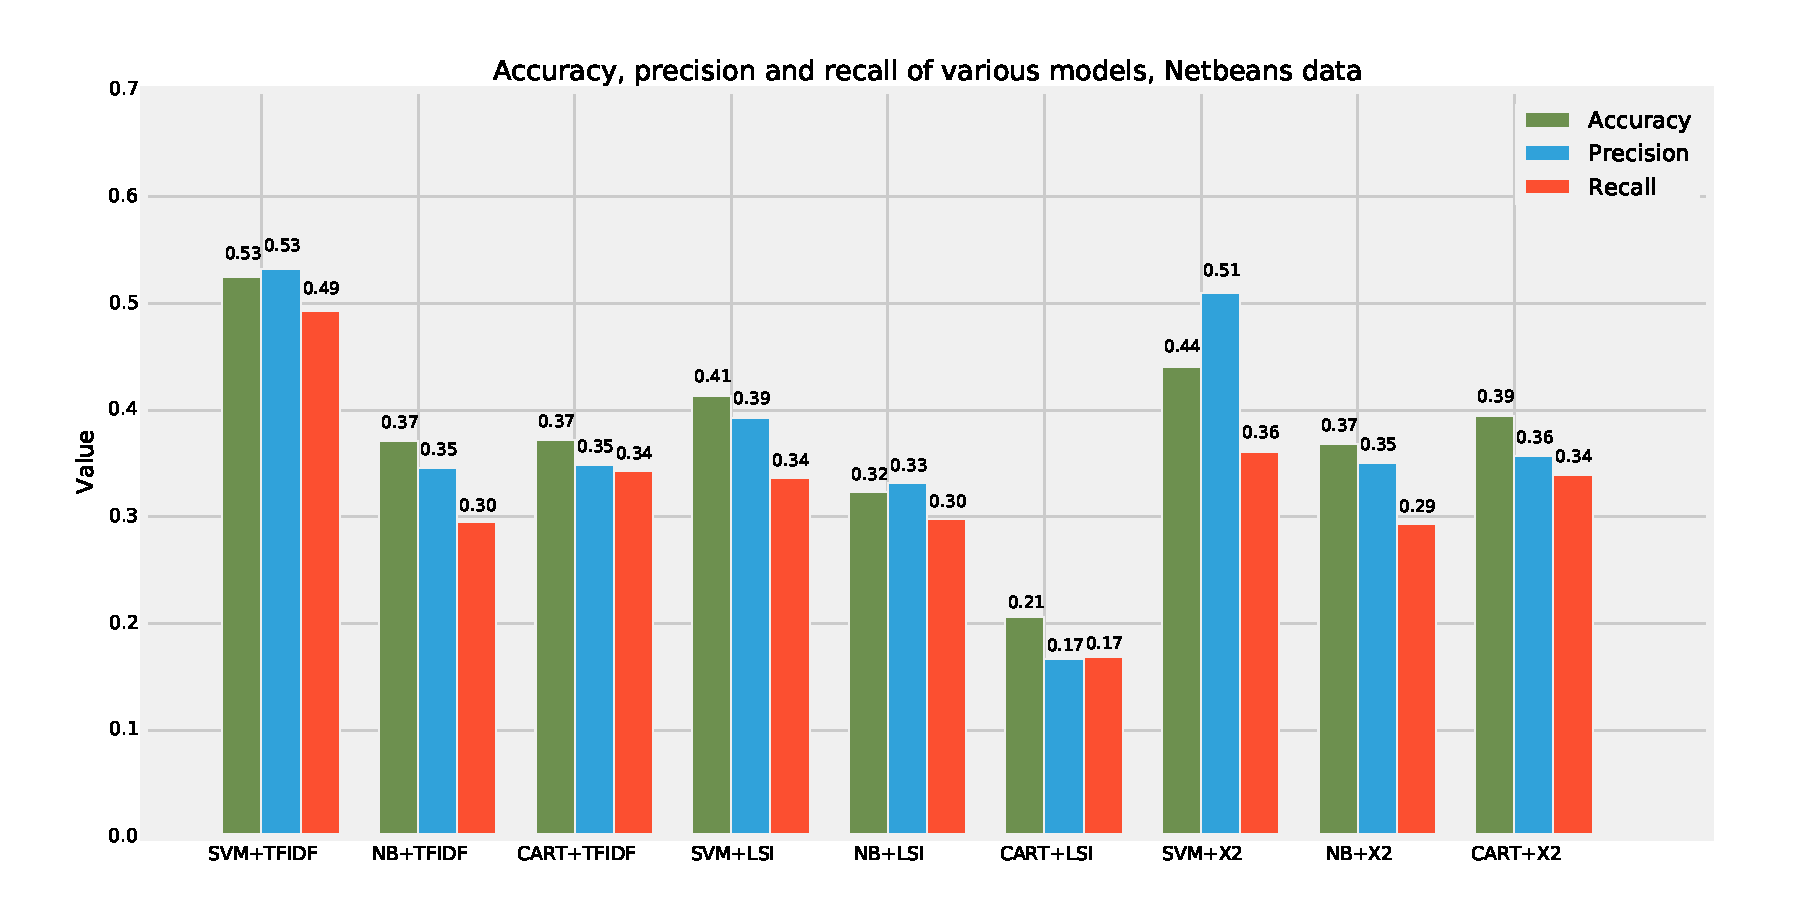
\includegraphics[width=\textwidth]{./images/comparison_of_models/netbeans.pdf}
    \caption{Comparison of models on Netbeans data.}
    \label{fig:results.models.netbeans}
\end{figure}

\subsection{Proprietary Data}

The proprietary data results are similar to the open-source datasets. Even in this case, the SVM model with TF-IDF offers the best performance of 53\% accuracy, 59\% precision and 47\% recall. The same model with LSI also shows quite a good performance and quite surprisingly, the Naive Bayes model with $\chi^2$ and TF-IDF performs quite well as far as precision is concerned. Both SVM and Naive Bayes models exhibit rather wide spreads between precision and recall values, which could be an indication of higher variance of the proprietary data (the distribution chart in section~\ref{section:datasets} seems to support this statement). Figure~\ref{fig:results.models.proprietary} presents the results in a graphical manner.

\begin{figure}[htbp]
    \centering
        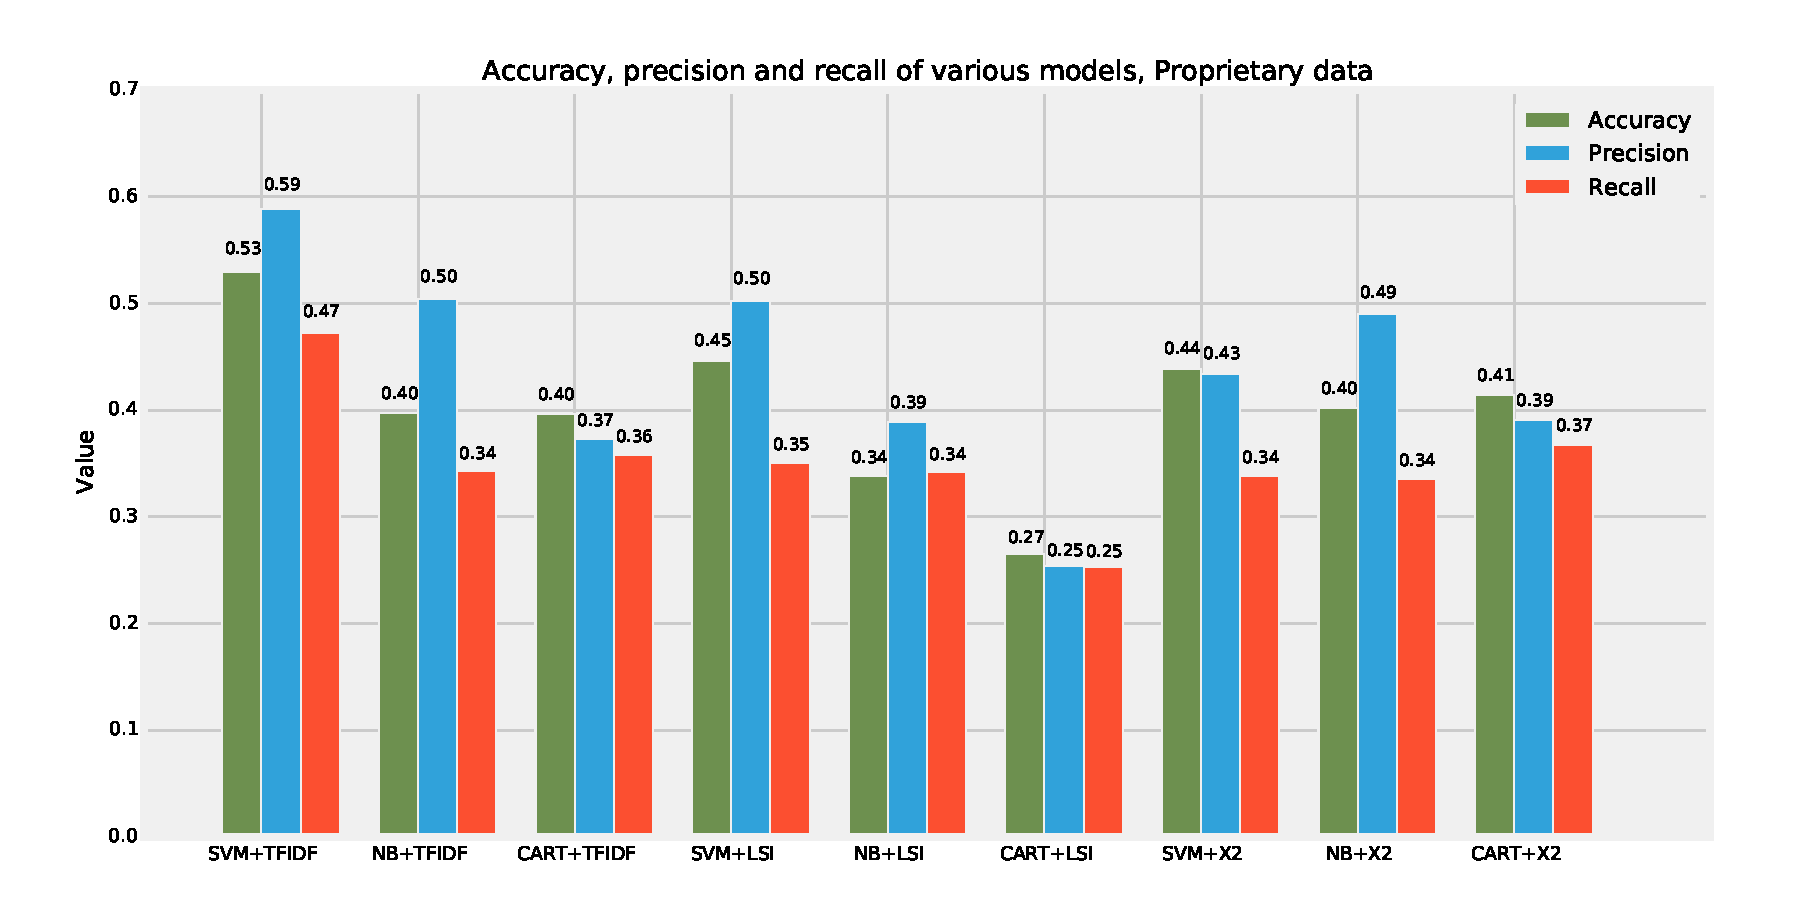
\includegraphics[width=\textwidth]{./images/comparison_of_models/proprietary.pdf}
    \caption{Comparison of models on the Proprietary data.}
    \label{fig:results.models.proprietary}
\end{figure}

\subsection{Conclusion}

The comparison shows that SVM with TF-IDF weighing performs best on all datasets. Not only that, it also generalizes very well, because there was no need to readjust the parameters of the model to get the best or nearly the best performance for all datasets. The disadvantage of the model is that it is the most computationally complex one, because SVM is the slowest of the three models as there are a lot of classes and  features. This can be at least partially dealt with by using $\chi^2$ feature extraction in conjunction with TF-IDF while sacrificing some of the performance.

The accuracy of all our models shows us how many times they are able to predict the correct assignee (\hyperlink{question:2}{Q2}). The precision and recall values of these models indicate that the models perform well even for unbalanced data (\hyperlink{question:3}{Q3}), there is, however, slight bias towards higher precision than recall. While the SVM model does not need different settings for different datasets and the NB and CART models do not have any, both LSI and $\chi^2$ feature extraction methods need to be tuned for each dataset to achieve the best performance (\hyperlink{question:4}{Q4}). It is therefore clear that the SVM model with TF-IDF has a huge advantage over all the other models we tested.

\section{Comparison of Datasets}
\label{section:comparison-of-datasets}

The main purpose of this section is to compare the proprietary dataset with the open-source dataset, providing an answer to question~\hyperlink{question:5}{5} of our application of GQM described in chapter~\ref{chapter:methodology}. In this question, we compare the proprietary dataset with only the Firefox dataset and we only use the Naive Bayes with now feature extraction method other than stop-words removal and SVM models with TF-IDF weighing.

We compare these two datasets by computing their performance (accuracy, precision and recall) for six different settings of the minimum \textit{issues per developers} requirement. These settings are: 1, 3, 5, 10, 20, 30. This allows us to see how the performance of the datasets changes when different number of developers (and bugs assigned to them) are removed. The narrower is the difference of the performance between the datasets for all the settings values, the higher is our confidence there is not much difference between open-source and proprietary data.

\subsection{Naive Bayes Model}

The first model for comparison is Naive Bayes. The only used feature extraction method for this model is stop-words removal.

First plot (Figure \ref{fig:results.datasets.nb_accuracy}) represents accuracy of the Naive Bayes model. You can see there are some interesting differences between the performances of the proprietary and open-source datasets. When the minimum requirement for issues per developer is 1, the accuracy of the proprietary dataset (33\%) is significantly higher than the accuracy of the open-source dataset (23\%). On the other hand, the accuracy of the proprietary dataset is higher for all settings of minimum issues per developer. When the requirement of issues per developers increases to 30, there is only 5\% difference between the accuracy of the proprietary dataset (40\%) and the open-source dataset (35\%).

\begin{figure}[htbp]
    \centering
        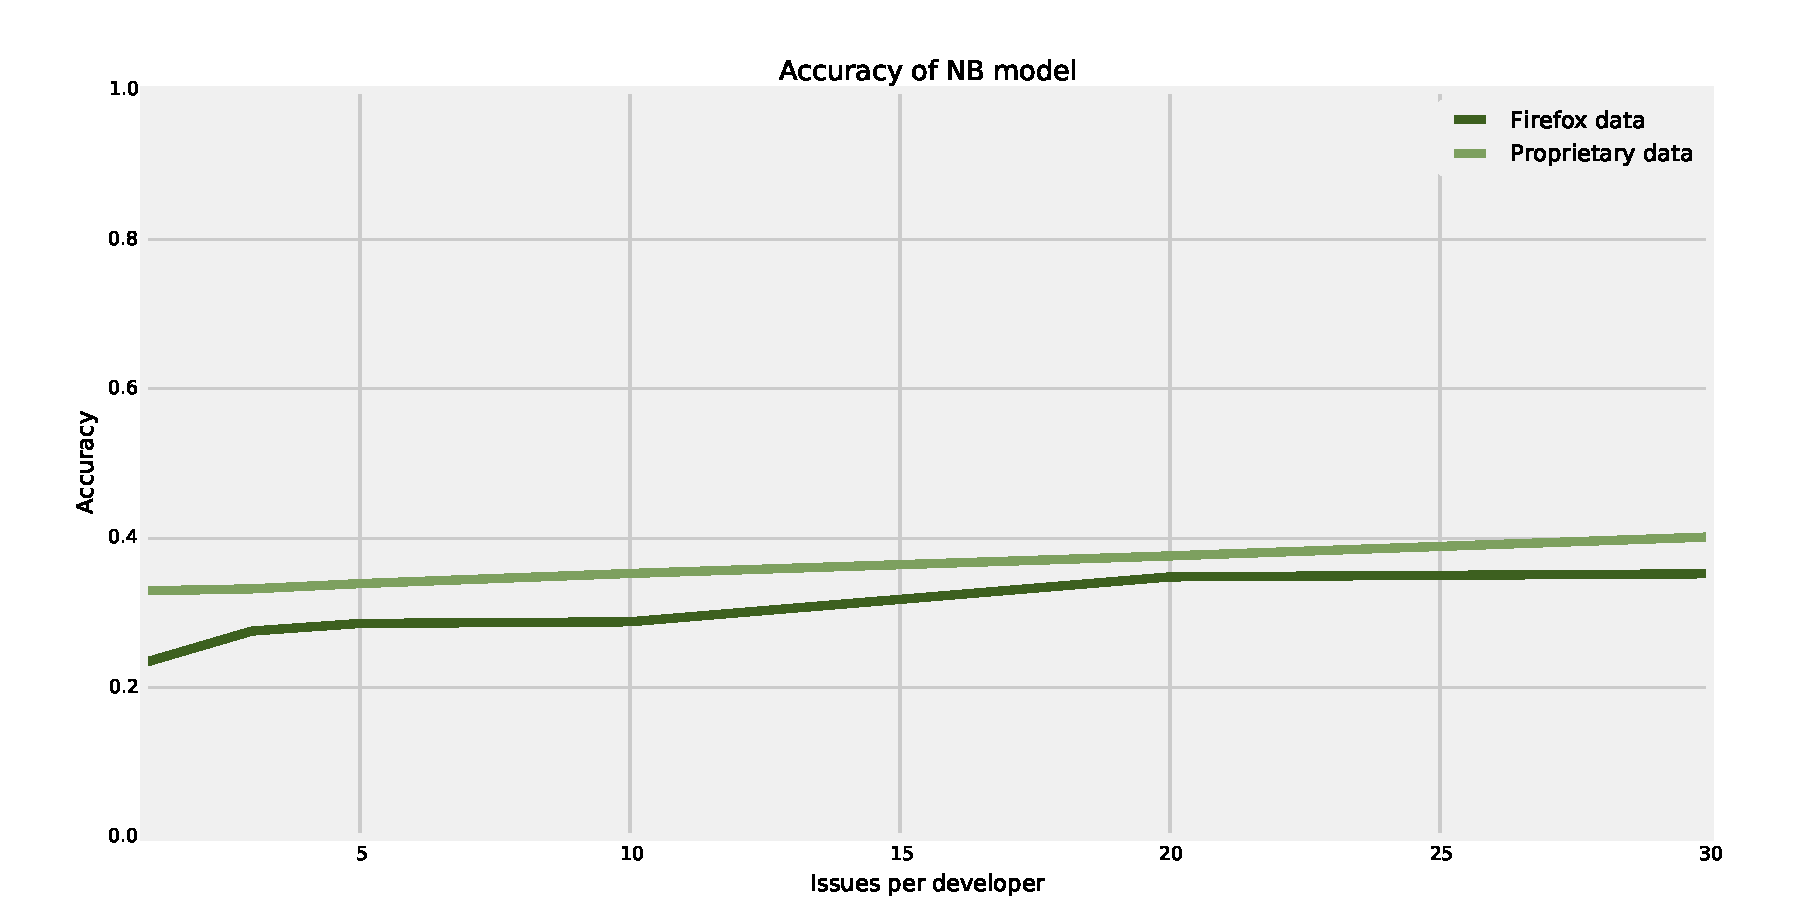
\includegraphics[width=\textwidth]{./images/prop_vs_os/nb_accuracy.pdf}
    \caption{Comparison of accuracy of Naive Bayes model.}
    \label{fig:results.datasets.nb_accuracy}
\end{figure}

Second plot (Figure \ref{fig:results.datasets.nb_pr}) shows the precision and recall values of the same model. Precision of the classifier for minimum issues per developer equal to 30 is 47\% and 49\% for the open source and proprietary data, respectively. Recall value is 29\% for the open source data and 33\% for the proprietary data in this settings. For minimum requirement of issues per developer from 1 to 10, we again see the interesting discrepancy observed in the accuracy plot. While the precision of the proprietary dataset begins with 20\%, the precision of the open-source begins with mere 7\%, almost three times lower. The difference between recall values is also staggering as it begins almost three times lower for the open-source dataset (14\% vs 5\%).

\begin{figure}[htbp]
    \centering
        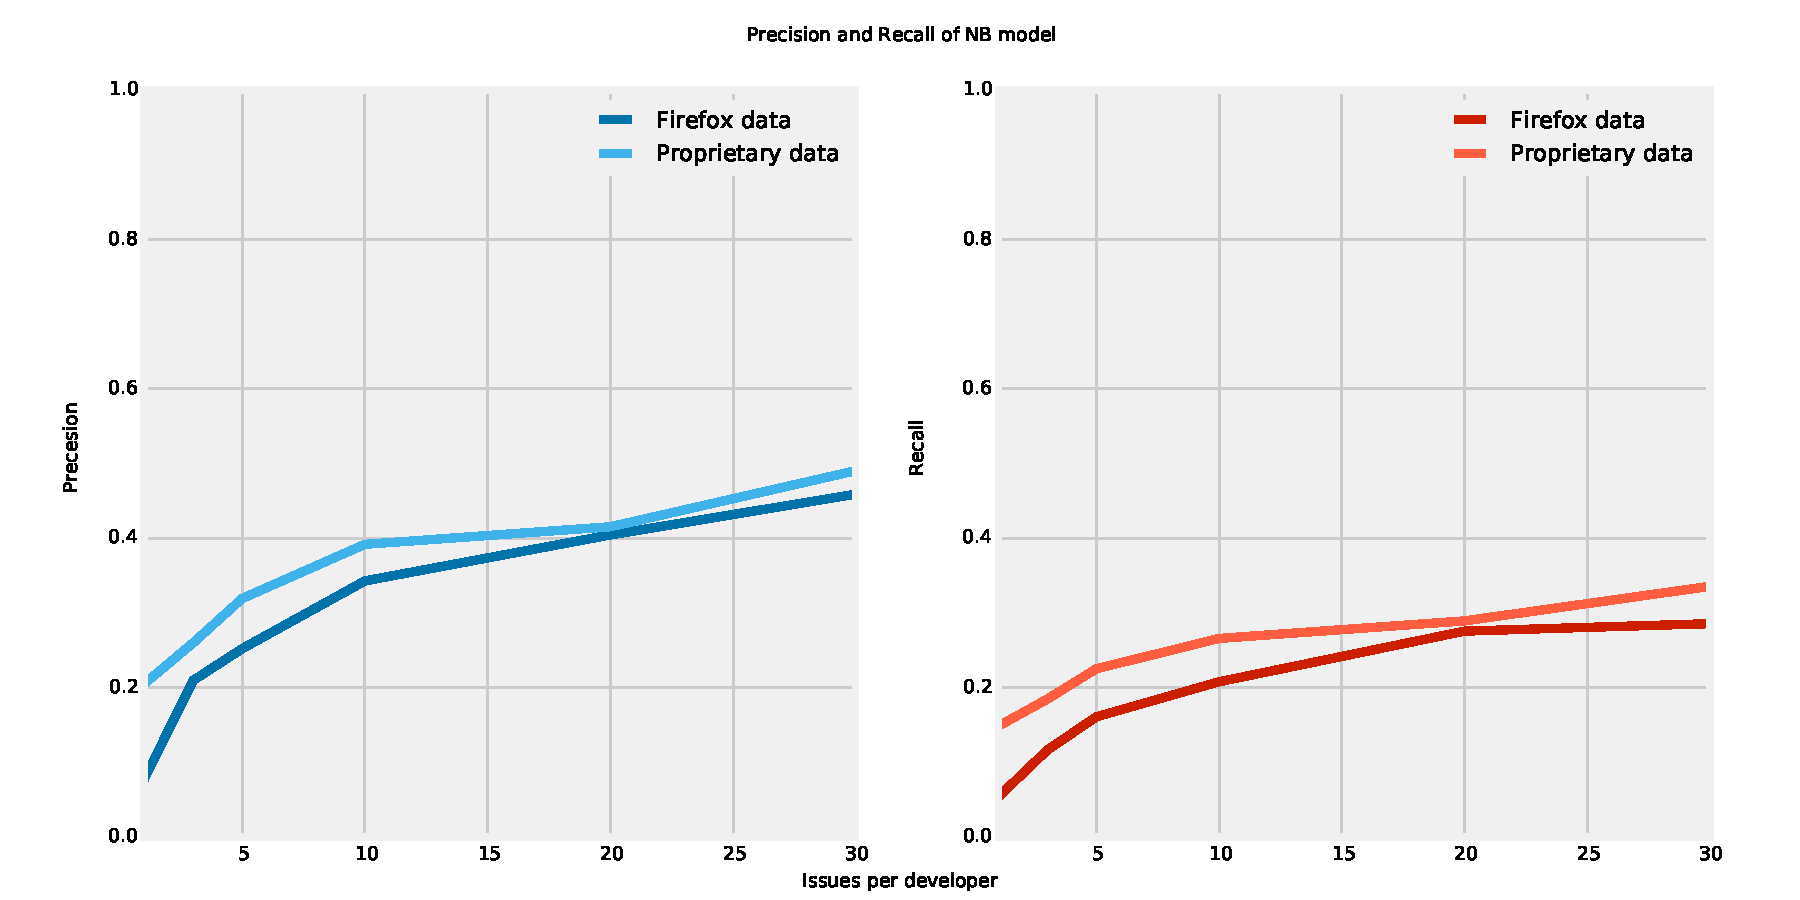
\includegraphics[width=\textwidth]{./images/prop_vs_os/nb_precision_and_recall.pdf}
    \caption{Comparison of precision and recall of Naive Bayes model.}
    \label{fig:results.datasets.nb_pr}
\end{figure}

\subsection{Support Vector Machine Model}

The second model used for comparison of the proprietary dataset with the open-source dataset is Support Vector Machine model with TF-IDF weighing and stop-words removal as this model shows the most promising results.

Figure \ref{fig:results.datasets.svm_accuracy} visualizes accuracy comparison of the model. While the accuracy of the proprietary dataset (53\%) is a bit lower than the accuracy of the open-source dataset (54\%) when minimum issues per developer equals 30 and while the value of this measure is about the same for all different values of issues per developer greater than 10, it begins again significantly higher for the proprietary dataset (42\%) than the open-source dataset (29\%). This difference cannot even partially be explained the same way we explained it in the Naive Bayes case as the accuracy difference eventually clears.

\begin{figure}[htbp]
    \centering
        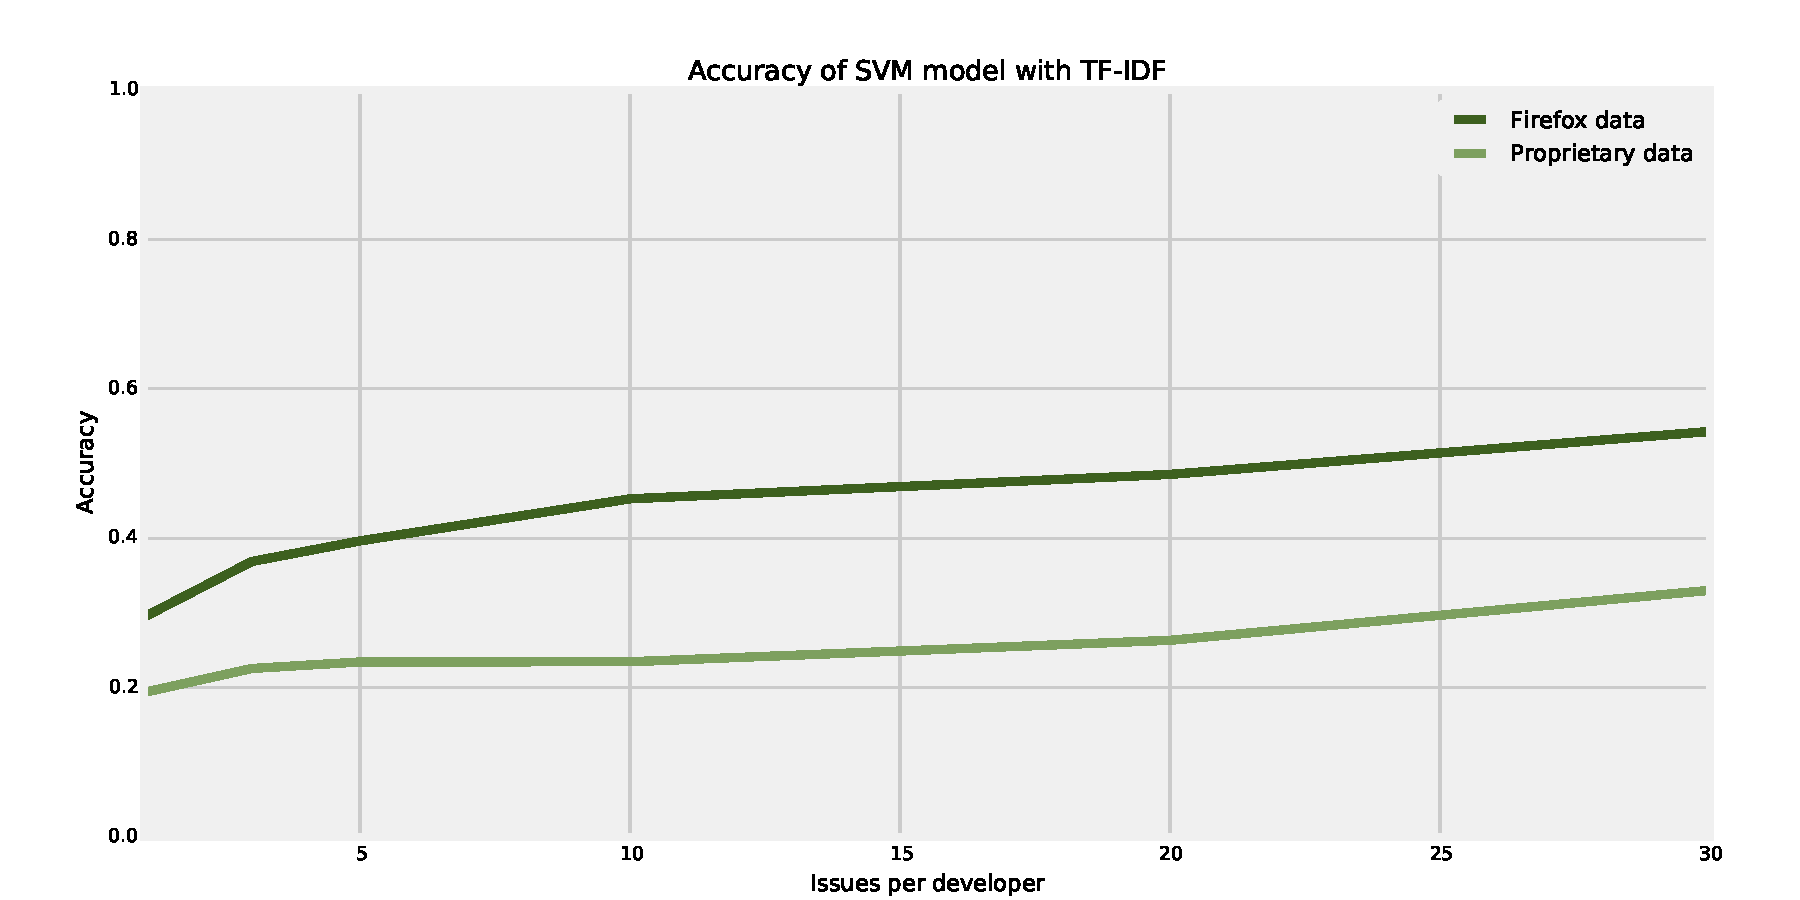
\includegraphics[width=\textwidth]{./images/prop_vs_os/svm_accuracy.pdf}
    \caption{Comparison of accuracy of SVM model.}
    \label{fig:results.datasets.svm_accuracy}
\end{figure}

Precision and recall of the SVM model is pictured on figure \ref{fig:results.datasets.svm_pr}. This plot, once again, confirms the hypothesis that the performance of the proprietary dataset begins much higher than the performance of the open-source dataset. The precision value of the proprietary dataset is eventually higher (59\%) than the precision value of the open-source dataset (54\%), but the difference at the beginning is just too overwhelming to be explained simply by the difference in performance overall (15\% vs mere 3\%). In the recall case, the right-most case (minimum number of issues per development requirement equal to 30) shows the performance of the proprietary dataset slightly lower (47\%) than that of the open-source dataset (50\%), even in this case, however, the performance for minimum number of issues per development equal to 1 is much higher for the proprietary dataset (14\% vs 3\%).

\begin{figure}[htbp]
    \centering
        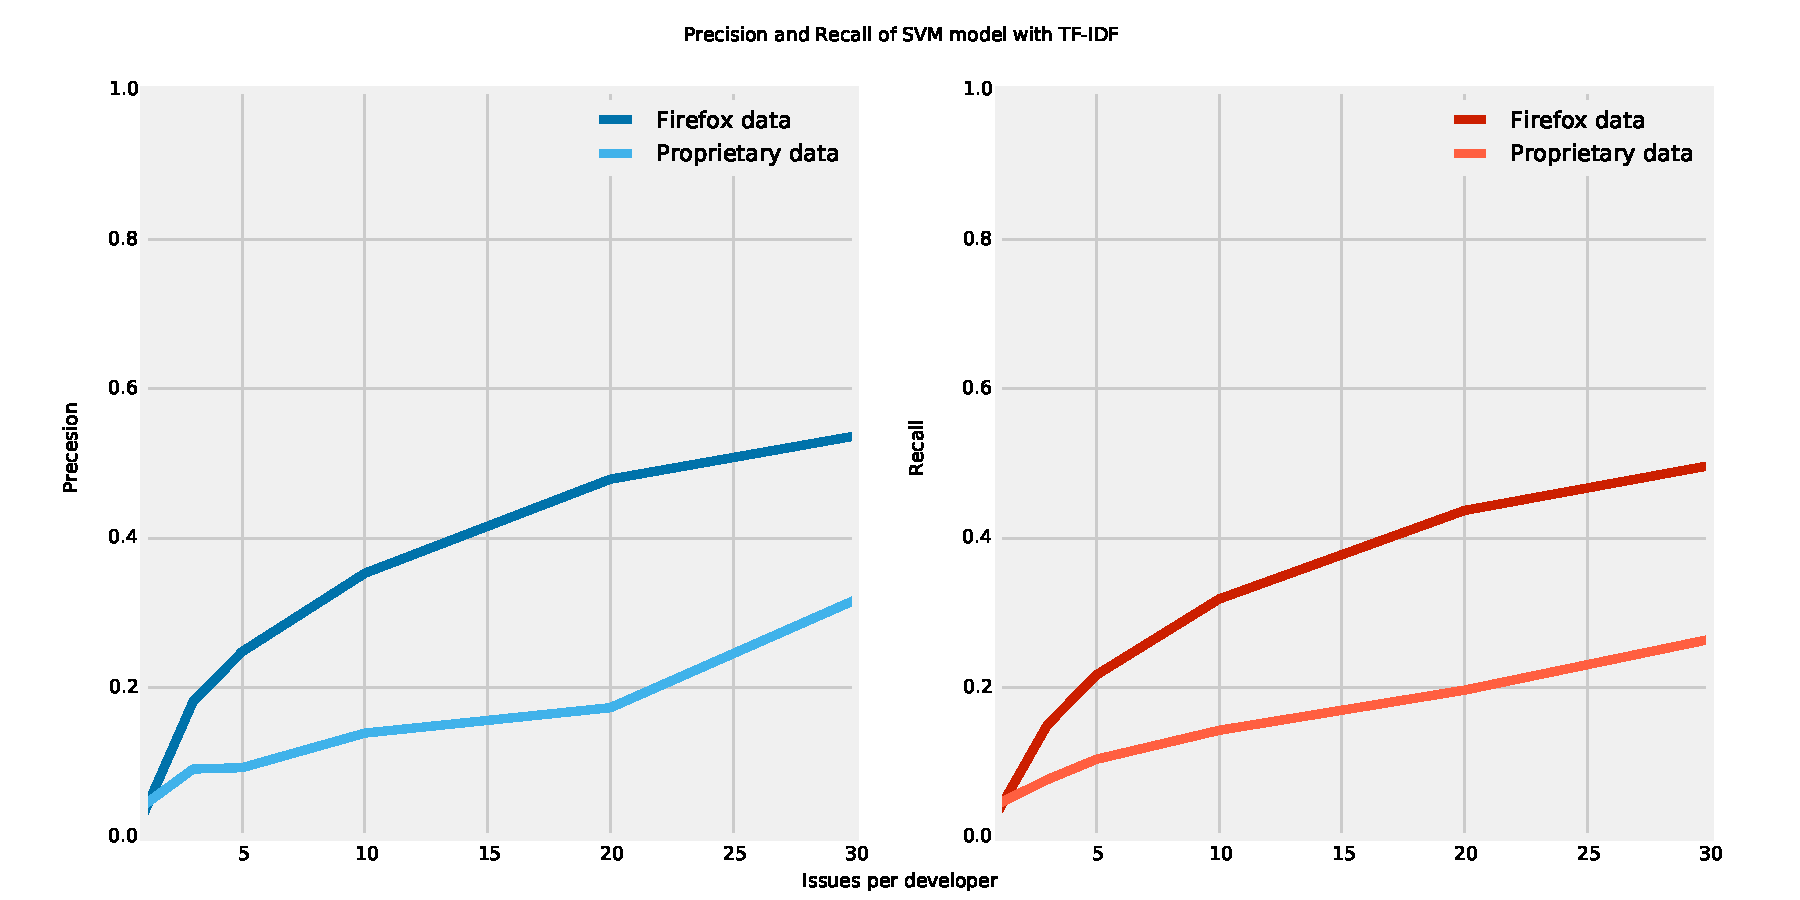
\includegraphics[width=\textwidth]{./images/prop_vs_os/svm_precision_and_recall.pdf}
    \caption{Comparison of precision of SVM model.}
    \label{fig:results.datasets.svm_pr}
\end{figure}

\subsection{Conclusion}

The results presented in this section suggest an interesting outcome. The performance of the proprietary dataset is generally quite similar to that of the open-source dataset at least as far as the accuracy of the SVM model is concerned. The Naive Bayes model seems to favor the proprietary dataset, however. Another interesting conclusion is that the spread between precision and recall is much higher for the proprietary dataset. This possibly implies higher variance of the dataset. The most striking result, however, emerges when the minimum number of issues per developers equals 1.

In terms of GQM defined in chapter~\ref{chapter:methodology}, we are now talking about question~\hyperlink{question:5}{5}. All our results show significant difference in performance for minimum number of issues per developers equal to 1. The much higher performance for the proprietary dataset in this regard can be probably explained by a simple fact---open-source bug repositories are open to anyone. It is logical to assume that a lot of bug reports in an open-source bug repository are fixed by random users that have never fixed bugs in the project, or fixed only a few of them---and only several users are actively maintaining the project. Proprietary projects are rarely open to public and it is therefore very unlikely there are many one-time assignees.

\section{Performance for Higher Number of Recommendations}
\label{section:compare-number-of-recommendations}

We look at the performance of the models for higher number of recommendations than one in this section. The plots will show the performance of the SVM model with TF-IDF weighing trained on the proprietary and Firefox datasets for number of recommendations from 1 to 10. In terms of GQM defined in chapter~\ref{chapter:methodology}, this section answers question~\hyperlink{question:7}{7}.

\subsection{Support Vector Machine Model}

For this comparison, we use the SVM model with TF-IDF weighing and stop-words removed. Figure \ref{fig:results.topx.svm_accuracy} shows how the accuracy increases with the number of recommendations, which is expected as the more there are recommendation, the higher the chance of a hit is.

\begin{figure}[htbp]
    \centering
        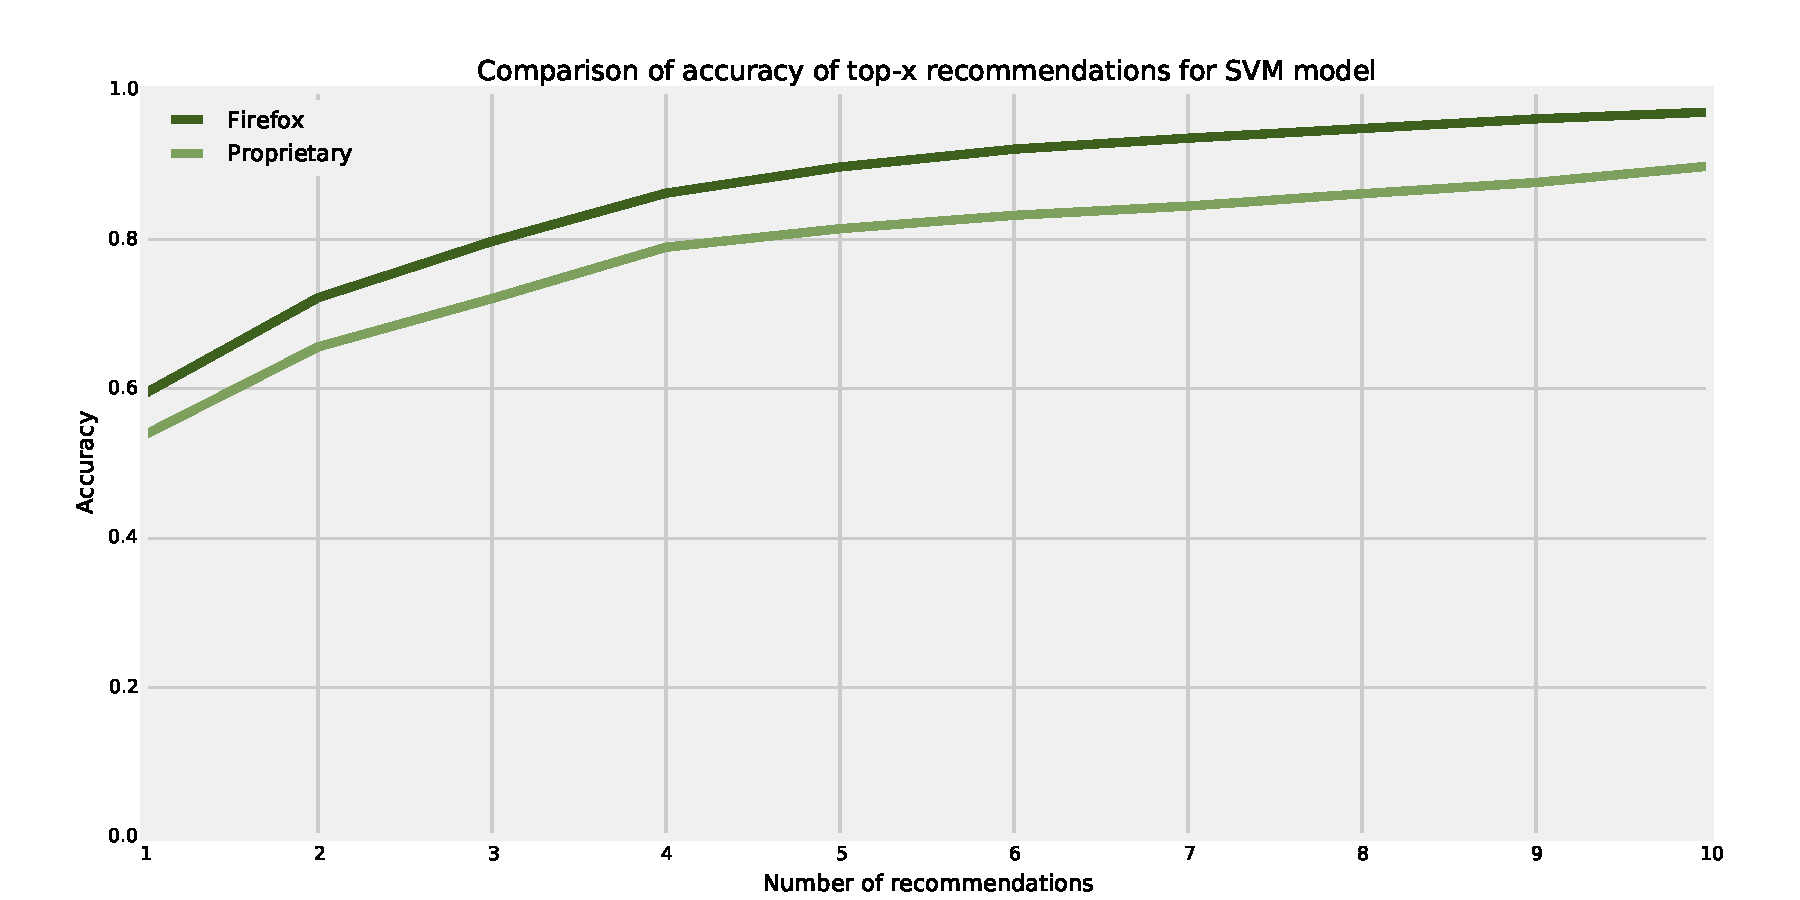
\includegraphics[width=\textwidth]{./images/top_x_comparison/svm_accuracy.pdf}
    \caption{Comparison of accuracy of top-x recommendations for SVM model.}
    \label{fig:results.topx.svm_accuracy}
\end{figure}

It is apparent from the plot that the highest performance boost happens when the number of recommendations changes from one to two both for the proprietary dataset (54\% vs 66\%) and the Firefox dataset (59\% vs 72\%). The accuracy of the Firefox dataset is equal to 90\% for 5 recommendations and 81\% for proprietary dataset. When the number of recommendations is 10, the performance is 97\% and 90\% for the Firefox and proprietary data respectively.

\subsection{Conclusion}

From the results in this section, we conclude that the highest number of recommendations to suggest to users that makes sense is 5. The performance does not increase very much with more recommendations and it would probably only lead to confusion if the number of recommendations was too high.

 \chapter{Discussions}

In this chapter, we discuss the results and compare them with related works (see \autoref{chapter:related-work}). We also address some possible threats to validity and conclude the chapter with potential future work.

\section{Results}

In the beginning of \autoref{chapter:evaluation}, we analyzed the three datasets that support our subsequent evaluation of the models. The distribution of the datasets seen in \autoref{section:datasets} seems to be very similar and thus it is not surprising that we fail to reject both following hypotheses. In terms of our GQM \hyperlink{question:4}{question 4}, this suggests that our model should work with all datasets without the need to tune the model's parameters. Subsequent evaluation of performance of the datasets supports this conclusion further. It is, however, possible, that some highly specific datasets would not work very well or not at all and it would therefore be necessary to adjust some of the parameters of our classifier.

The distribution of the datasets in \autoref{section:datasets} and the consecutive testing of hypotheses also addresses \hyperlink{question:5}{question 5}. From this single point of view, it would seem there is almost no difference between open-source and proprietary data. In term of performance, however, there is a significant difference as can be seen in \autoref{section:comparison-of-datasets}. One possible explanation could be the size of the window that was used to select the training and testing samples of bug reports. If the window is too big, the developers that have a high number of resolved tickets but are no longer active could be considered by the model for future prediction and disadvantage the other developers that are currently active. This explanation does not seem to hold to our analysis as can be seen in \autoref{section:window-size}. As it was tested on open-source data, it is possible that the proprietary data are more sensitive to the window size. Second possible explanation could be bad quality of the proprietary data. It is, for example, possible, that the open source community pays more attention to ticket triage. Be it as it may, we can safely conclude that there is a difference between our samples of open-source and proprietary data albeit only in terms of performance.

As mentioned above, we evaluate \hyperlink{question:6}{question 6} in \autoref{section:window-size}. We employed three approaches to answer this question and while there was some variations in performance with respect to the size of the window, there was not found a trend that would warrant a conclusion in one way or another with high enough confidence. Even though the results do seem to suggest that the size of the window does not significantly change the performance of the classifier, it would be necessary to do a more thorough analysis with more than three approaches on more datasets to adopt this outcome with more confidence.

In \autoref{section:baseline}, we saw that our model outperforms the baseline model, which tells us that automatic ticket triage based on supervised text classification does work at least to some extent (\hyperlink{question:1}{question 1}). In the subsequent sections, we determined what model is the best in our case and what its performance is answering \hyperlink{question:2}{question 2}. We can also answered \hyperlink{question:3}{question 3} by evaluating precision and recall of the classifier. It is not very surprising that the Support Vector Machine model performs best as it was already concluded in many other works\todo{citation needed}. On the other hand, our selection of possible models is quite limited so while unlikely, it is possible that there are models that can outperform SVM on some or most of our datasets.

The last part (\autoref{section:compare-number-of-recommendations}) of our evaluation addresses the question of recommending more than one assignee for one bug report (\hyperlink{question:7}{question 7}). It is possible to assign a developer to a bug report automatically without any input from the reporter (or project manager) apart from the summary and description simply by having the classifier choose the most probable candidate. This way, the user who manages tickets has to rely on the computer generated model to successfully choose the correct developer. If that is not achieved, the bug report has to be reassigned to someone else. Another way is to utilize a semi-automated approach which presents the user with a list of suggestions rather than automatically filling in the best match. The question is how many developers to show in such a list without overwhelming the user with too many choices. The best approach might be to consider the change in performance, if the performance does not change much when the number of recommendations is changed from five to ten, it might not be sensible to recommend ten developers. One the other hand, it makes sense to change the number of suggestions to five if the performance increases significantly after recommending five possible assignees rather than two.

\section{Threats to Validity}

When doing research, it is quite often the case that the used approach has some questionable aspects. In this section, we discuss these aspects in depth starting with the metrics used for evaluation and continuing with the way the data is preprocessed, and finally the testing.

The three metrics used for evaluation have certain problems that should be kept in mind. All together, they are quite a good way to measure the performance of a machine learning model. Separately, however, they have to be treated with certain skepticism. Accuracy is the most obvious metric when measuring how many times the correct answer is picked. There are many cases where this metric could be very misleading. One such case is when the labels of a dataset are heavily biased towards a single class. Let's say that the dataset contains samples and 90\% of them are assigned the same label. In such a case, the classifier could always predict the same label (in this case, the label that is assigned to 90\% data samples) and easily achieve 90\% accuracy. If the label with these properties is the positive class, even precision would measure the same result. And recall would result in 100\%. It is therefore necessary to establish a baseline that for example always predicts the most frequent class and consider accuracy in terms of the accuracy achieved by the chosen baseline. In our case, we achieved accuracy 18\% on Firefox data with our baseline while the accuracy of our best model on the same dataset is 57\%. This is a relatively good result considering the performance of the baseline. On the other hand, it is still possible the model always chooses between only several classes instead of considering them all. 

In our evaluation, we also use precision and recall (both macro-averaged). These metrics must always be considered together as it is possible to achieve 100\% precision or recall if the datasets contains samples with only one class. Using macro-averaged variant of precision and recall makes this sort of misleading result somewhat less likely, it is not, however, eliminated altogether. Considering the baseline results for precision and recall, any bias towards a single class or several classes seems improbable but it cannot be ruled out. It should be kept in mind that these metrics are very theoretical and the reality can be a lot different.

Before our data is used for training, it is randomly shuffled. This increases the performance by as much as 8\%. We decided to shuffle the data beforehand to get more accurate results~\todo{add a reason why data is shuffled or add a section somewhere and make a reference}. This might be quite misleading, however. In reality, the classifier is used to predict a label for a new sample that was not created in the past. The new sample is usually as close to the time window of the training test as possible therefore the bias should not be too big. It is likely the most accurate result is somewhere between the results of the classifier trained on non-shuffled and then shuffled data.

The accuracy of our results can also by threatened by the way it is tested. We test our models only once, it is unfortunately the case that each test produces slightly different results sometimes by as much as 4\%. There are two reasons for this. First reason is the shuffling of the data as mentioned above. The way the models work makes them sensitive to the order of the data. Another reason is the way the models operate themselves. The implementation of the SVM model, for example, randomly selects the best optimization for each iteration and it is of course not guaranteed each SVM session finds the most optimal results. This problem could be partially solved by training and testing the models more than once and using the expected value with confidence intervals instead of a raw value. Due to the time complexity of the models and the time it takes to do a single test, this extensive way of testing was not realized in our evaluation.

\section{Comparison with Related Works}

In this section, we attempt to compare our evaluation with related works. However, there are a couple of challenges that should be kept in mind. Some of the papers that we mention in chapter \ref{chapter:related-work} do not clearly define their evaluation process and even if they do, the differences in their process make it hard to draw a satisfactory conclusion. Another problem is that the sources of the datasets used by us and them do not always match, and even if they do, it is unlikely they are from the same time window. It is our belief, based on the window analysis we did in chapter \ref{chapter:evaluation}, that the effect of different time windows on measured performance should be quite small. Lastly, some of the papers we mention in chapter \ref{chapter:related-work} do not use the same metrics for evaluation. For these reasons, we compare our results with the results of only the papers we find sufficiently similar as far as the process, datasets and metrics are concerned.

First, we compare our results with Anvik et al.~\cite{Anvik2006}. In their evaluation, they were able to achieve precision 64\% and recall only 2\%. We were able to achieve precision 51\% and recall 45\%. There are a couple of differences, however. We used a dataset with 3,000 bug reports, they used 9,752. They also used a different approach of filtering inactive developers. The difference in recall can be probably attributed to the way it is calculated by Anvik.

Another study with which we compare our results is Alenezi et al.~\cite{Alenezi2013}, who used a Naive Bayes on several datasets as well as on Netbeans. The best results they achieved are with $\chi^2$ feature extraction -- precision of 50\% and recall of 21\%. We achieved precision value 53\% and recall 49\% with SVM and TF-IDF. There are two major differences. Our dataset contains 3,000 bug reports while their contains 11,311. The other major difference is that while we remove developers that have not fixed at least 30 bugs, they remove developers that have not fixed at least 25 bugs in the last year.

Lastly, we compare our evaluation results with the work of Xia et al.~\cite{Xia2015} They employed an interesting learning algorithm multi-label k-nearest neighbor classifier (ML-kNN) and topic modeling using Latent Dirichlet Allocation (LDA). The datasets they used include Netbeans (26,000 samples) which makes it easier to compare with our results for Netbeans (3,000 samples). Their precision and recall values for top-5 recommendations are 32\% and 71\% respectively, while our precision and recall values for top-1 recommendation are 53\% and 49\%.

As mentioned in the beginning of this section, it is complicated to draw a conclusion when our processes, evaluations and datasets differ so much. We can, however, conclude that both our and their results are similar which implies our process is at least as good as theirs. 
 \chapter{Conclusion}

The primary objective of our thesis was to find the best model for supervised text classification of automatic ticket triage in order to achieve the best practical result for a web application requested by a privet Czech-based software company. We have concluded that the best classification model is SVM with TF--IDF---achieving accuracy of 57\%, precision of 51\% and recall of 45\% with Firefox dataset---53\%, 53\% and 49\% with Netbeans dataset---and finally 53\%, 59\% and 47\% with the private company dataset. The secondary objective of our thesis was to find out whether the best model can be applied to all projects without optimizing the parameters. Our analysis and evaluation helped us determine that while some classification models do require optimization of the model's parameters for each project, our best model (SVM with TF--IDF) does not suffer this drawback.

Another important objective of our thesis was to find out if there is a difference between open-source and proprietary data. Our analysis of the datasets and evaluation of the models showed that there is a difference especially when comparing the performance of the datasets without filtering developers with little activity as a lot of bug reports in an open-source repository are resolved by one-time users (users that are not actively maintaining the project and fixed only a few bugs).

Future work could extend several aspects of our thesis. We have attempted to discover whether it is auspicious to pay attention to the size of the time window within which the samples form a training dataset had been created. While our results are for the most part inconclusive, it seems plausible that the size of a time window affects the performance of a classification model. Another aspect of our thesis that could be extended is the evaluation process. The measured results exhibit quite a lot of variance and it would therefore be more accurate to evaluate each model several times in order to compute the mean value possibly with confidence intervals. The set of used metrics could possibly be extended as well with metrics like AUC and ROC.

Machine learning and text classification are still quite young disciplines and only our recent technologies provided us with enough computational power to drive the research in these fields of study further. Our results, while satisfactory in the context of the related work, can almost certainly be improved with different, possibly yet undiscovered, techniques and methods---because if a human can predict an assingee for a bug report with higher accuracy than our classification model (which they almost certainly can), so can a computer.


 \bibliographystyle{IEEEtran}
 \bibliography{thesis}

 \appendix
 \chapter{Extra Plots}
 \label{appendix:extra-plots}

 \section{Topic Analysis}

 \begin{figure}[htbp]
    \centering
        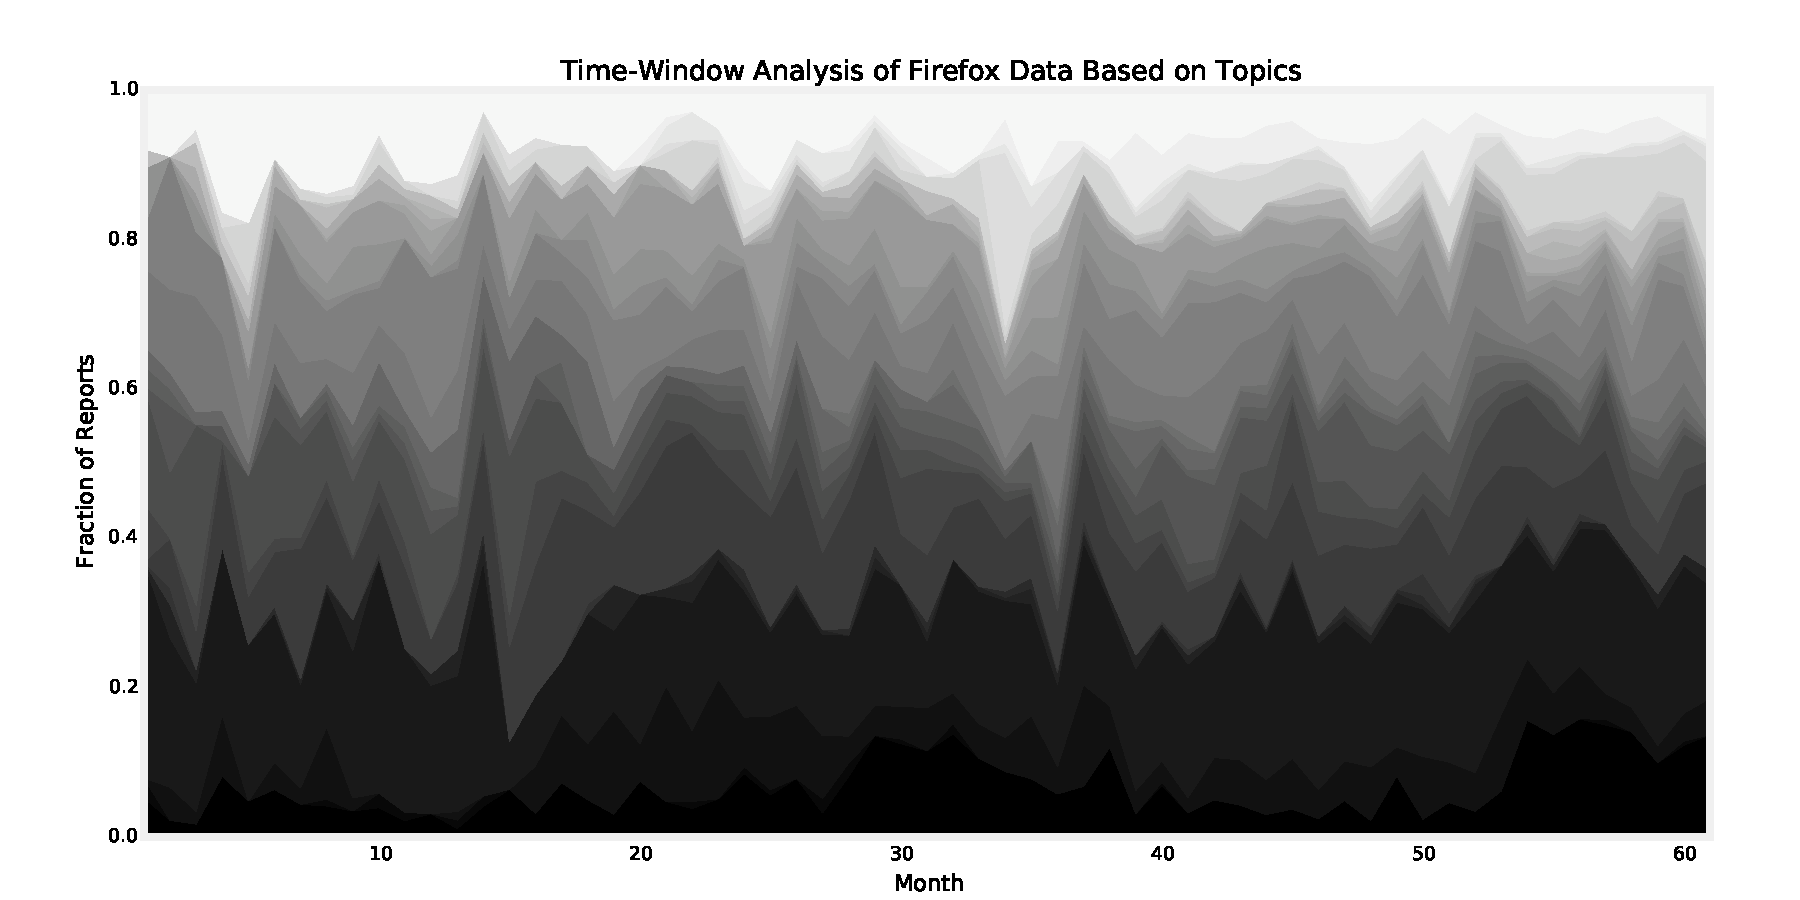
\includegraphics[width=340px]{./images/topic_component_distribution/firefox_topic.pdf}
    \caption{Topic Analysis of Firefox Data for 30 Topics}
    \label{fig:distribution.firefox.topic.30}
 \end{figure}

 \begin{figure}[htbp]
    \centering
        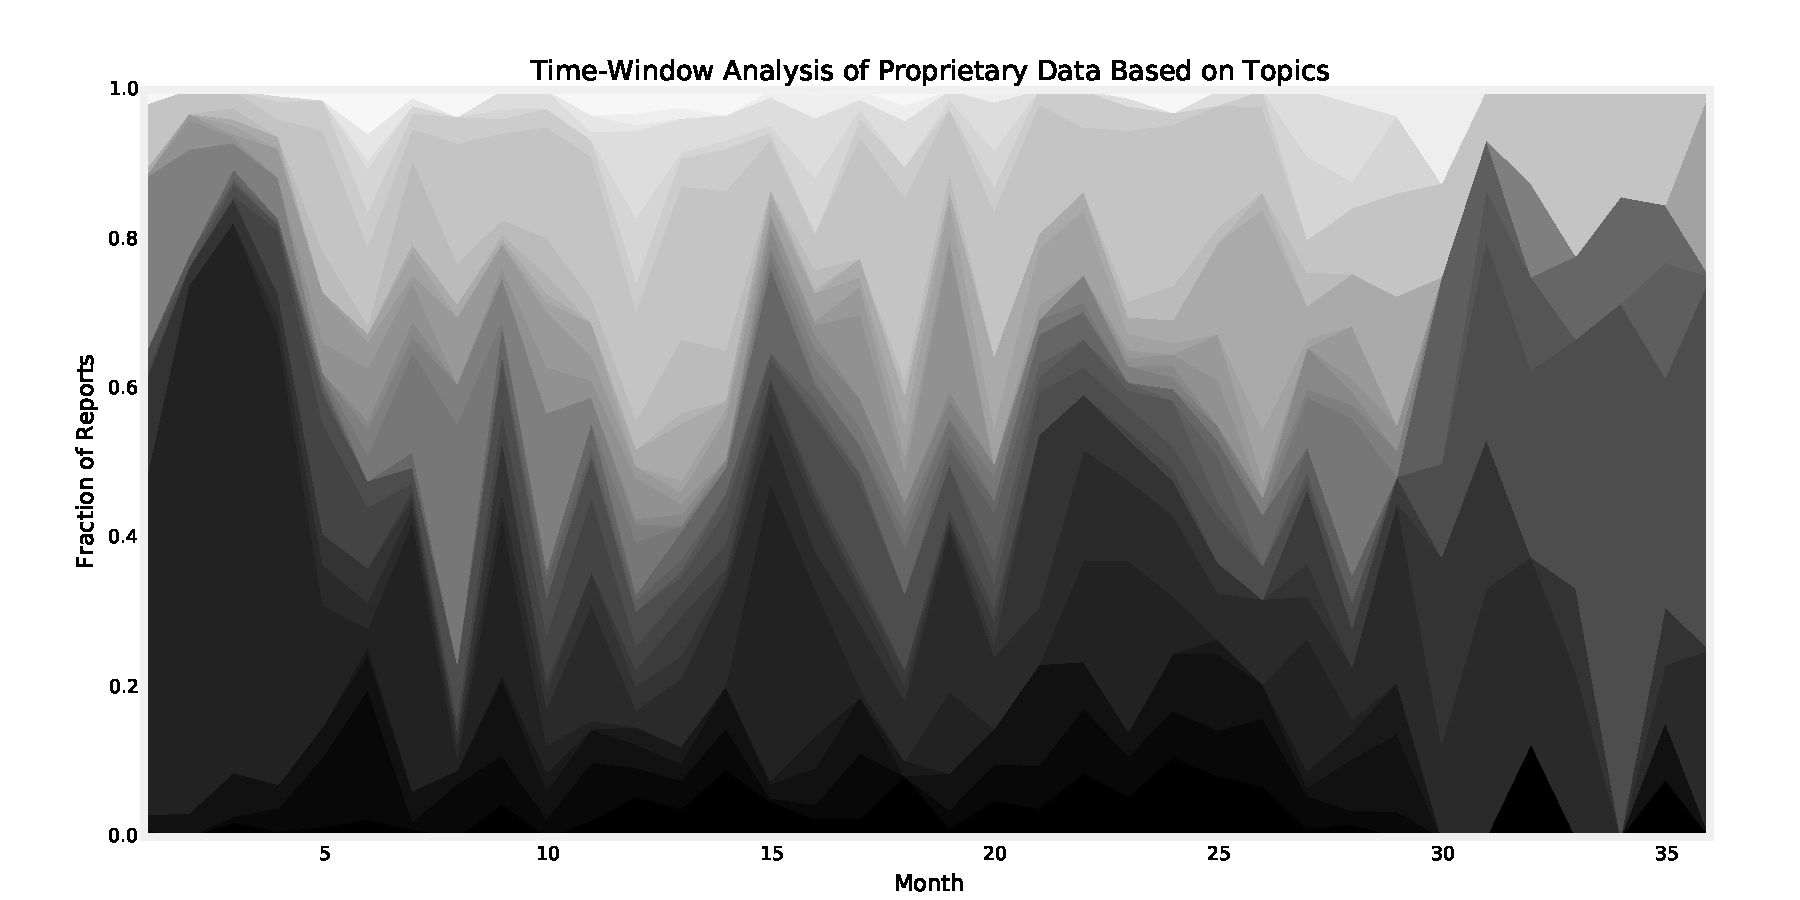
\includegraphics[width=340px]{./images/topic_component_distribution/proprietary_topic.pdf}
    \caption{Topic Analysis of Proprietary Data for 30 Topics}
    \label{fig:distribution.prop.topic.30}
 \end{figure}

 \clearpage
 \section{Baseline}

 \begin{figure}[htbp]
    \centering
        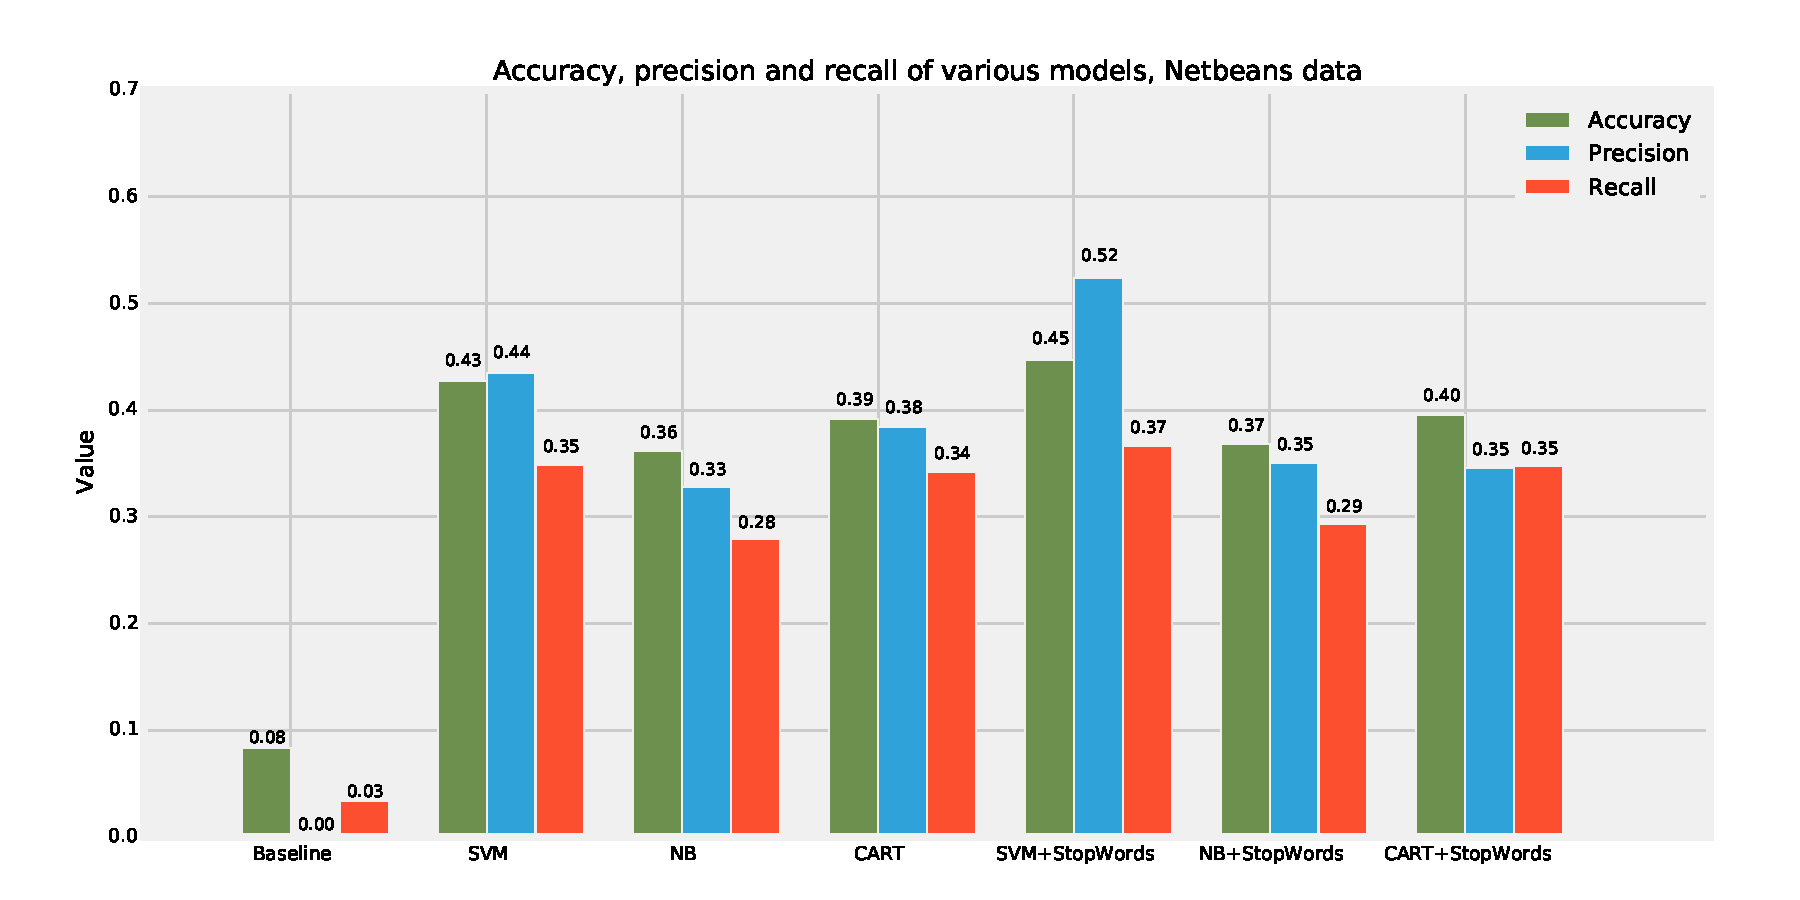
\includegraphics[width=340px]{./images/comparison_of_models/netbeans_0.pdf}
    \caption{Stop-Words removal on Netbeans data}
    \label{fig:baseline.netbeans}
 \end{figure}

 \begin{figure}[htbp]
    \centering
        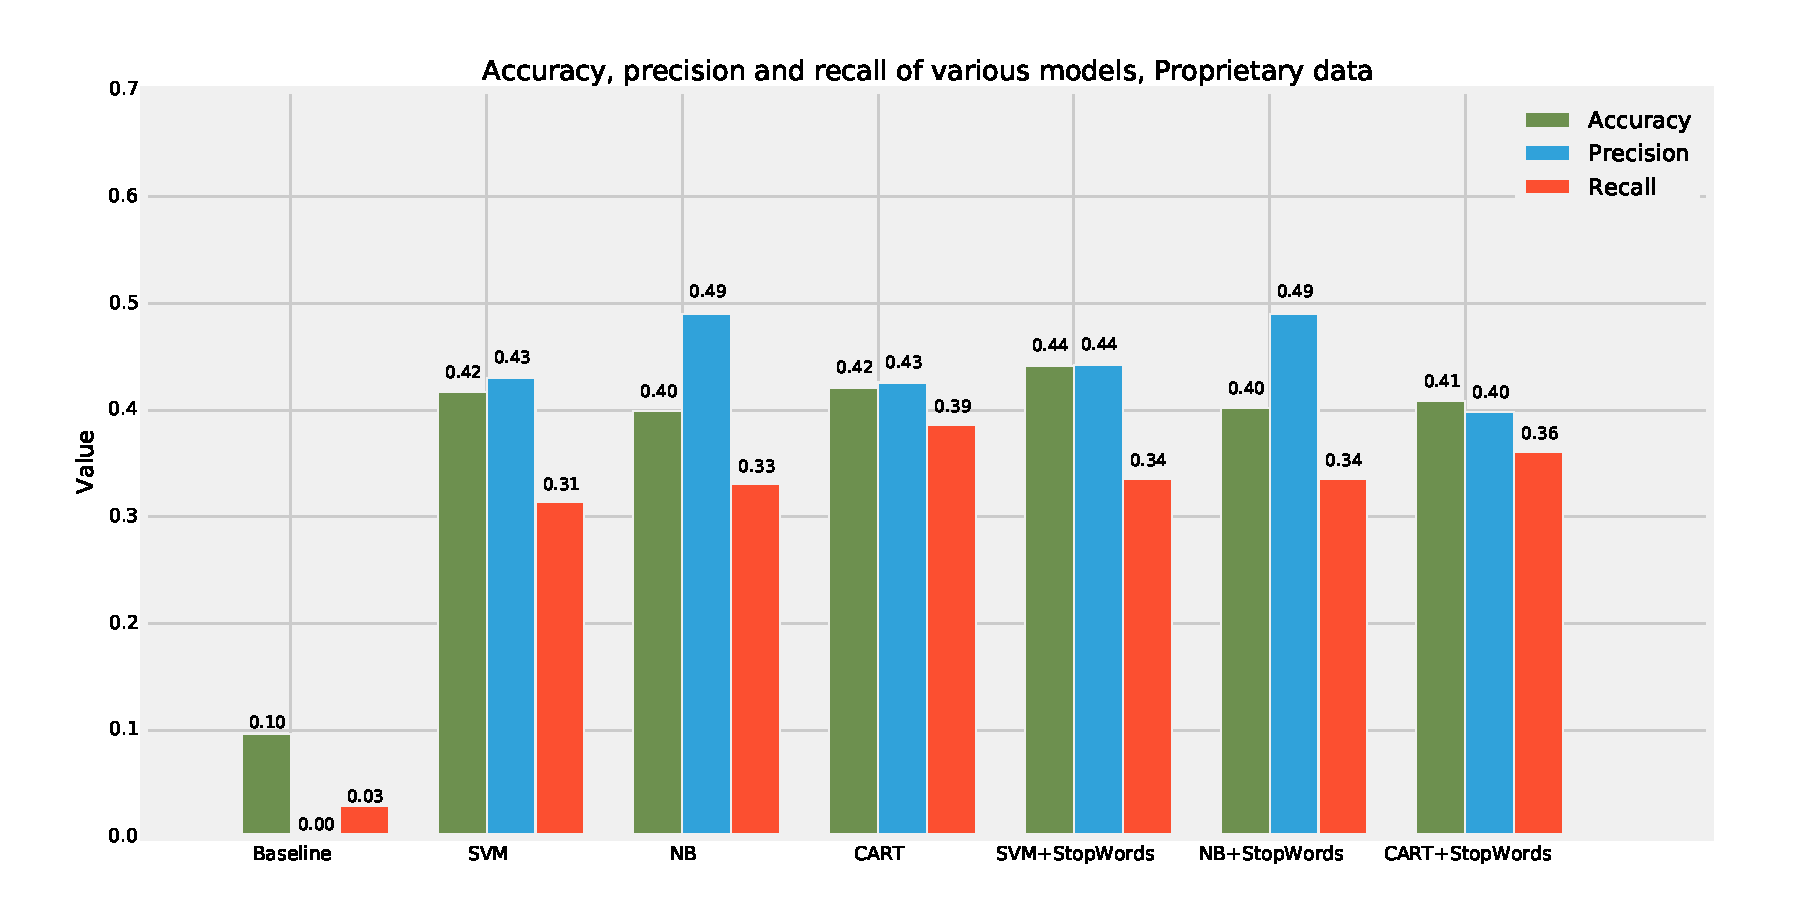
\includegraphics[width=340px]{./images/comparison_of_models/proprietary_0.pdf}
    \caption{Stop-Words removal on proprietary data}
    \label{fig:baseline.prop}
 \end{figure}

 \clearpage
 \section{Comparison of Datasets}

 \begin{figure}[htbp]
    \centering
        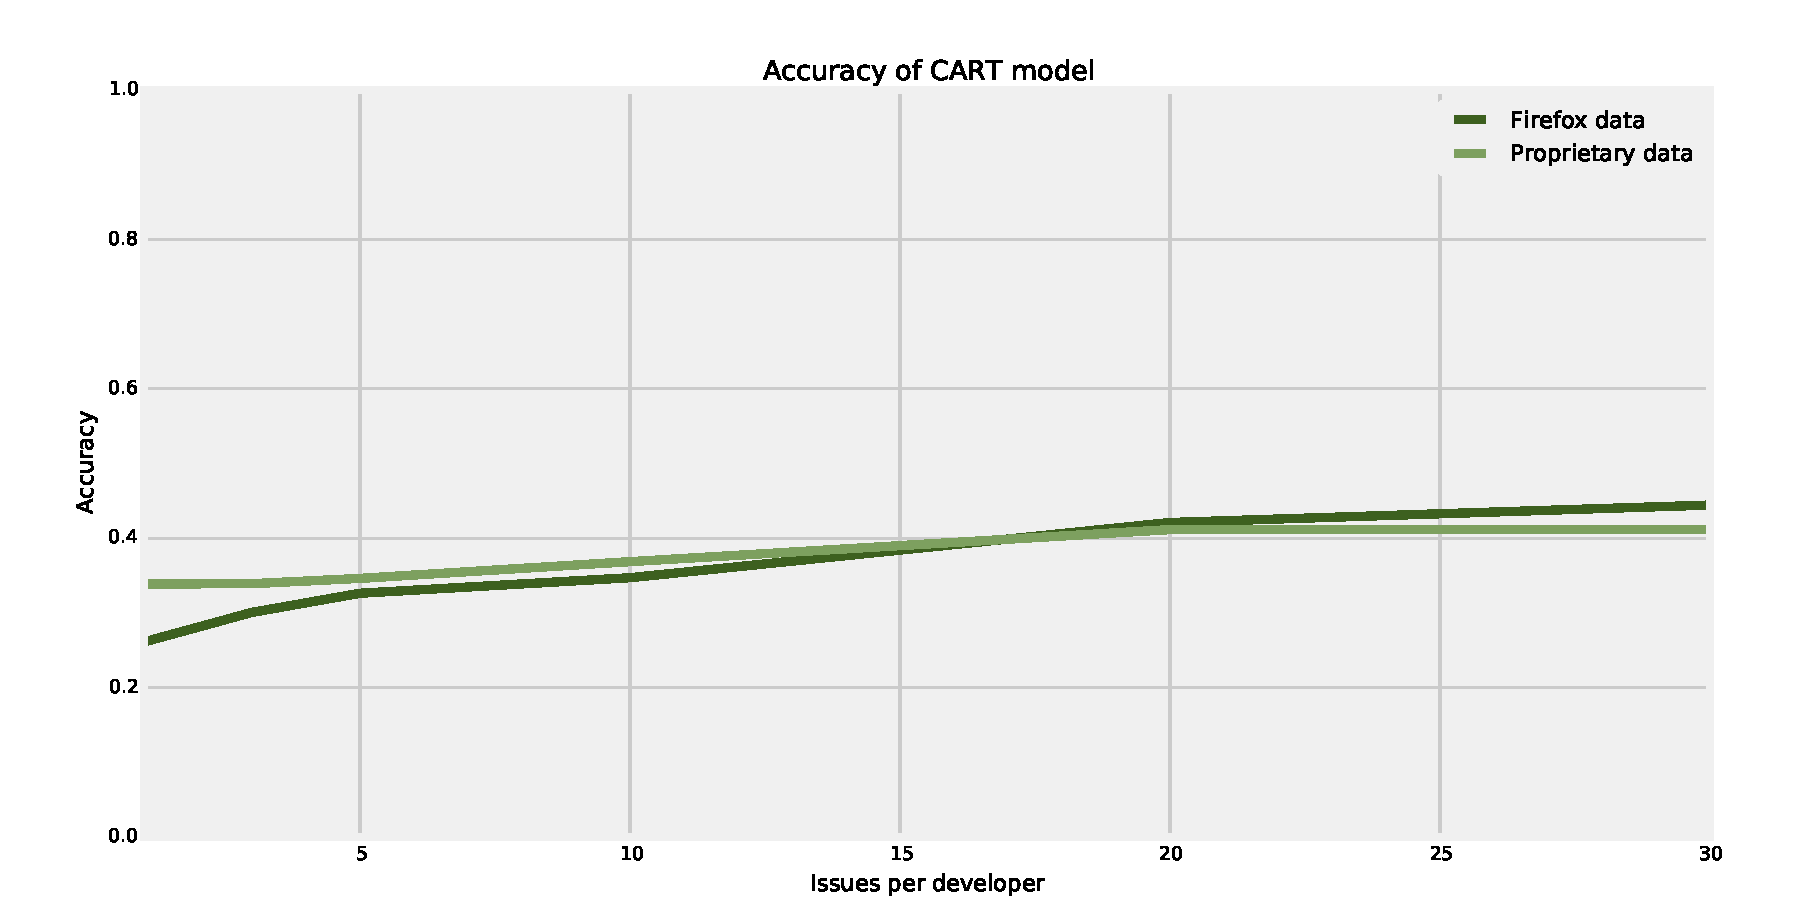
\includegraphics[width=340px]{./images/prop_vs_os/cart_accuracy.pdf}
    \caption{Comparison of accuracy of CART model.}
    \label{fig:results.datasets.cart_accuracy}
 \end{figure}

 \begin{figure}[htbp]
    \centering
        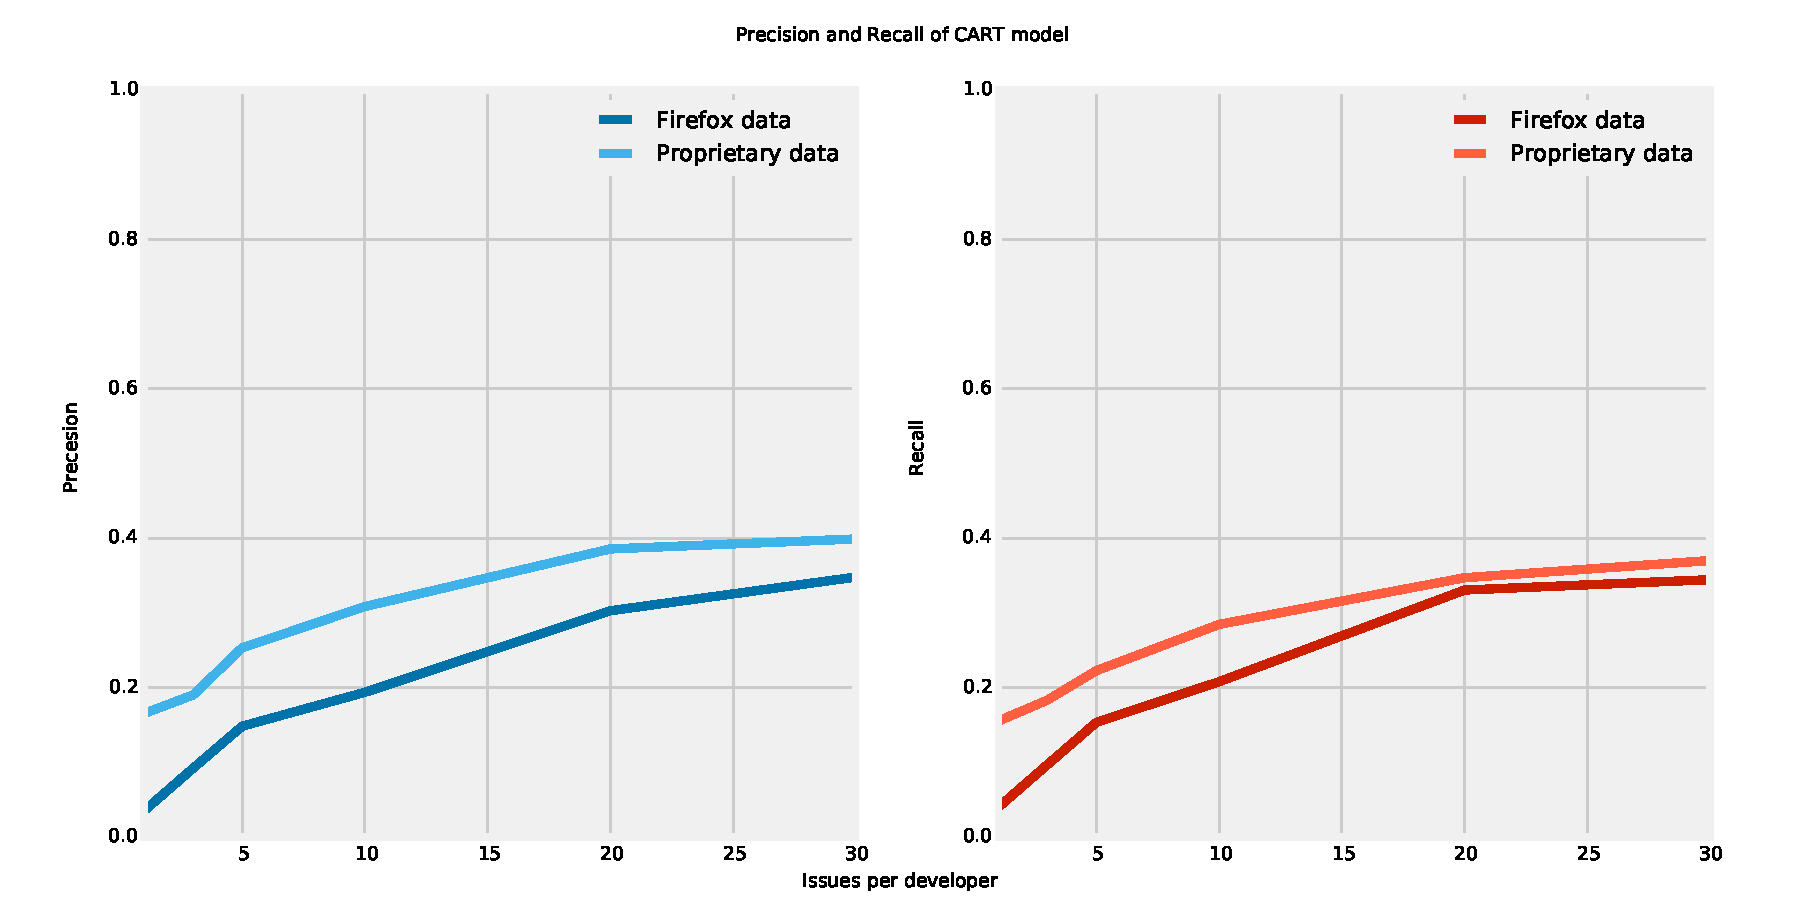
\includegraphics[width=340px]{./images/prop_vs_os/cart_precision_and_recall.pdf}
    \caption{Comparison of precision and recall of CART model.}
    \label{fig:results.datasets.cart_pr}
 \end{figure}

 \clearpage
 \section{Performance for Higher Number of Recommendations}

 \begin{figure}[htbp]
    \centering
        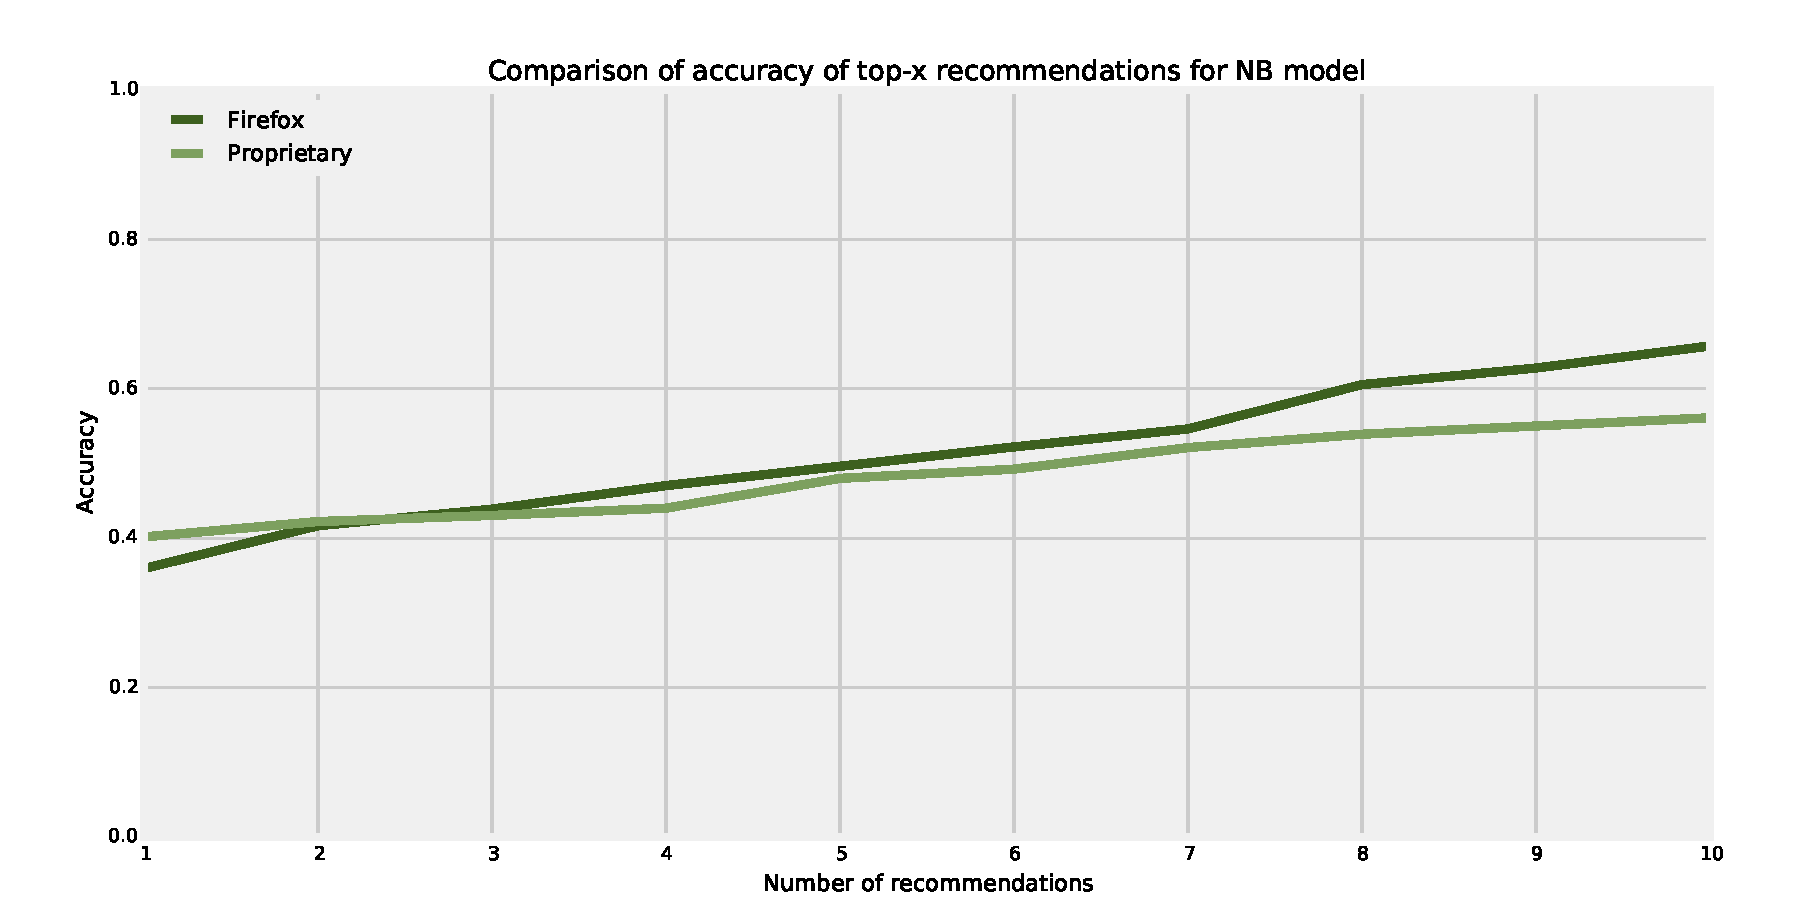
\includegraphics[width=335px]{./images/top_x_comparison/nb_accuracy.pdf}
    \caption{Comparison of accuracy (top-x) for NB model.}
    \label{fig:results.topx.nb_accuracy}
 \end{figure}

 \begin{figure}[htbp]
    \centering
        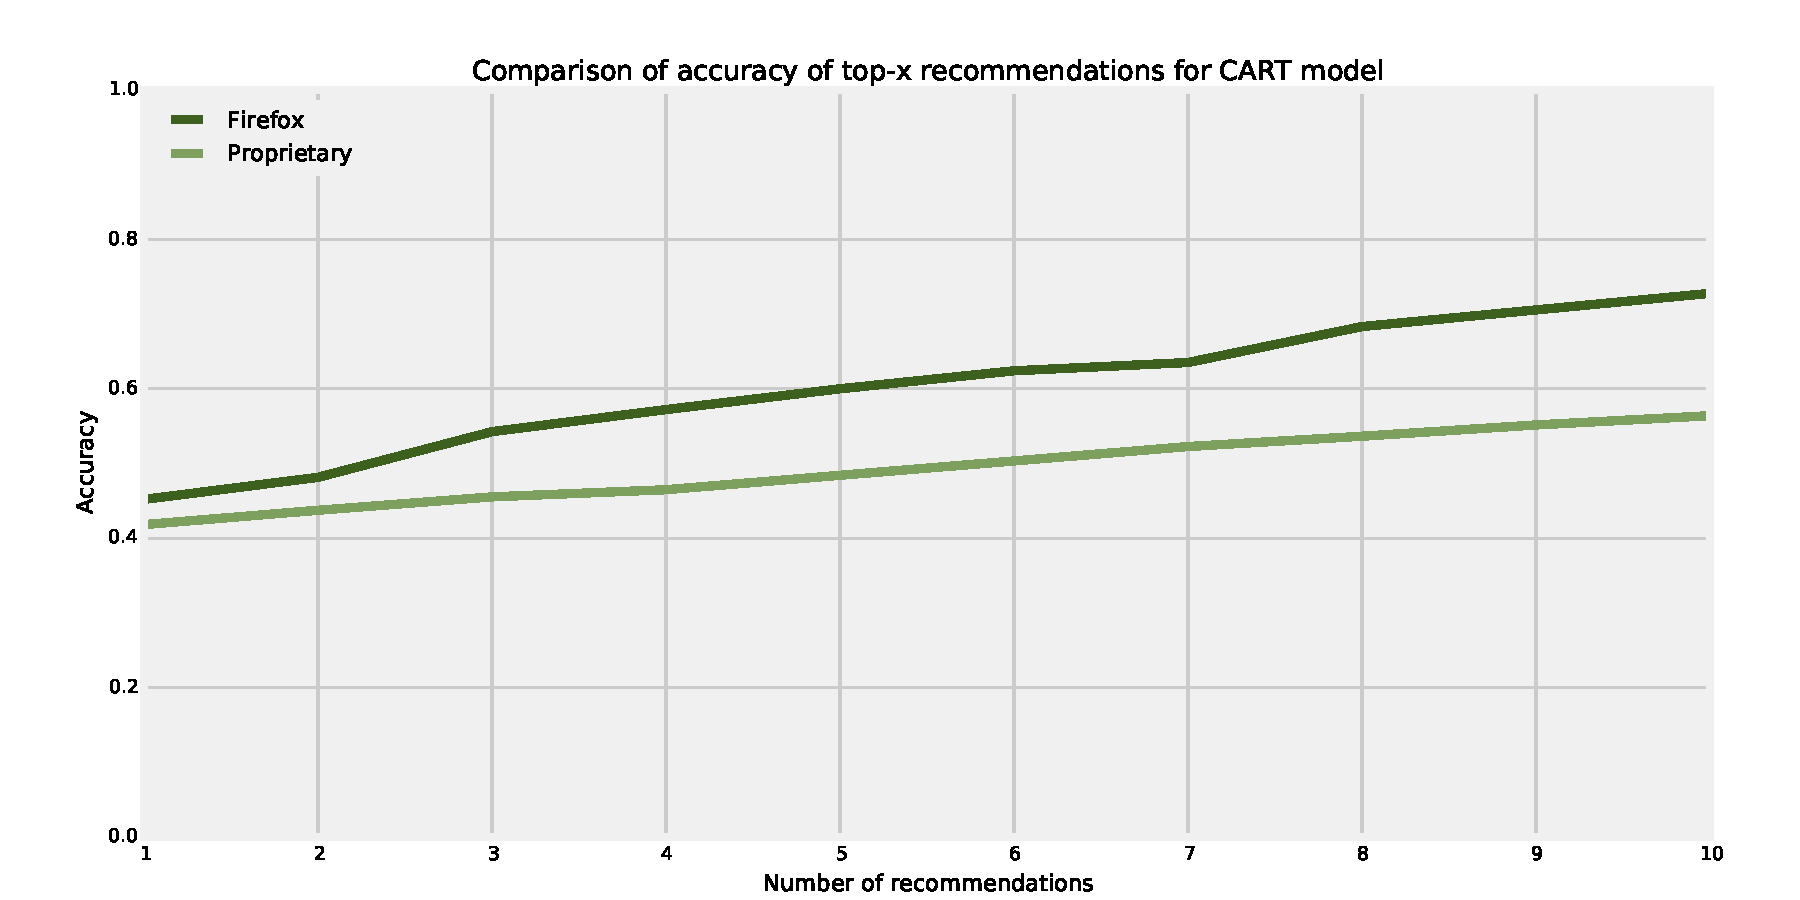
\includegraphics[width=335px]{./images/top_x_comparison/cart_accuracy.pdf}
    \caption{Comparison of accuracy (top-x) for CART model.}
    \label{fig:results.topx.cart_accuracy}
 \end{figure}

 \chapter{Links}
 \label{appendix:links}

 \section{GitHub Repositories}

 This section contains links to GitHub repositories created while working on this thesis. First link contains source code of the thesis text. Second link contains the source code of a web application that was created for the company that provided the proprietary dataset. The last link contains the source code of a Python library based on numpy, scikit-learn and scipy created for better usage of several ML models and feature extraction techniques.

 \begin{itemize}
   \item[Thesis text]: \url{https://github.com/VaclavDedik/masters-thesis}
   \item[Triager]: \url{https://github.com/VaclavDedik/triager}
   \item[Classifier]: \url{https://github.com/VaclavDedik/classifier}
 \end{itemize}

 \todos
\end{document}
